1000-- In which country did Albert Girard (1595-1632) die?

a$)$ Columbia \\
b$)$ France \\
c$)$ Netherlands \\
d$)$ Switzerland\\

Answer : c$)$\\

Feedback : \\
Albert Girard died in the Netherlands. He was the first to use the abreviations \og $\sin$\fg, \og $\tan$\fg\ and \og
$\sec$\fg\ to respectively designate the sine, the tangent line and
the secant.
The answer is c$)$.\\

        \begin{center}
        The Netherlands\\
    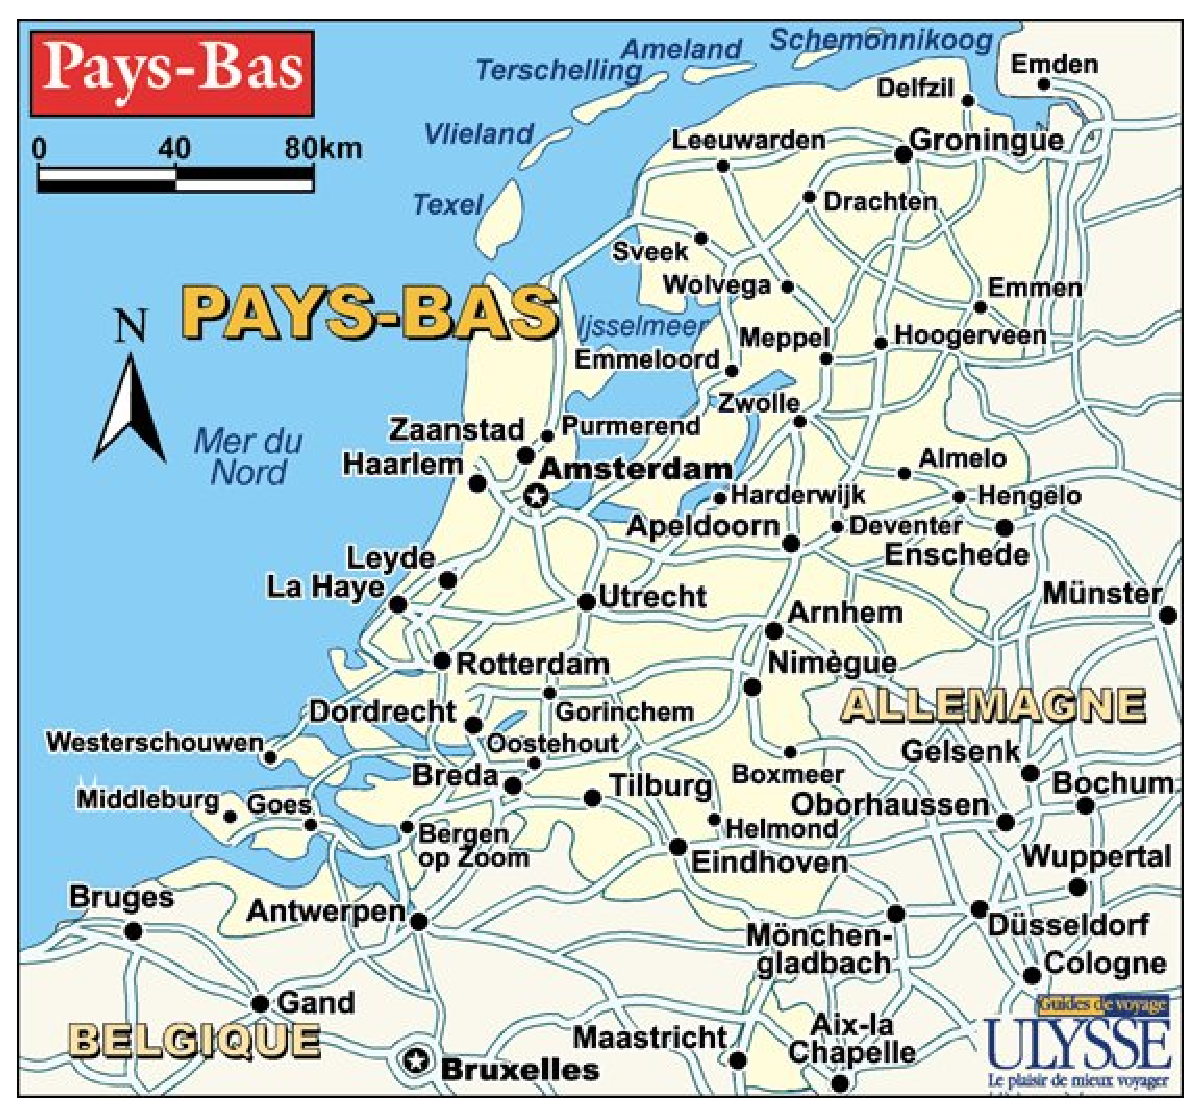
\includegraphics[width=6cm]{pays.eps}\\
    \end{center}

1001 * -- In 1629, Albert Girard set out, for the first time in history, the following theorem : {\sl Any equation of
degree $n$ has $n$ exact roots, \`provided that impossible roots are counted, each with its multiplicative order}.
Nowadays, what is the name of this theorem?

a$)$ {\sl Fundamental theorem of algebra} \\
b$)$ {\sl Fundamental theorem of arithmetic} \\
c$)$ {\sl Fundamental theorem of Chemistry} \\
d$)$ {\sl Fundamental theorem of the theory of numbers}\\

Answer : a$)$\\

Feedback : \\
Il is the fundamental theorem of algebra.
The answer is a$)$.\\

1002-- Who was the first to use the abreviations
\og$\sin$\fg, \og$\tan$\fg\ and \og$\sec$\fg\ to respectively designate the sine, the tangent line, and the secant?

a$)$ Albert Girard \\
b$)$ Edward Waring \\
c$)$ Johann Heinrich Lambert \\
d$)$ Marie Curie\\

Answer : a$)$\\

Feedback : \\
Albert Girard was the first to use these abreviations.
The answer is a$)$.\\

1003-- What is the most important work of Ren\'e Descarte,
in which he made the first steps toward the invariant theory?

a$)$ {\sl Thus spoke Zarathustra} \\
b$)$ {\sl The Geometry} \\
c$)$ {\sl Opticks} \\
d$)$ {\sl Philosophiae naturalis principia mathematica}\\

Answer : b$)$\\

Feedback : \\
It is Geometry or La G�om�trie}.
The answer is b$)$.\\

1004-- What was founded by Descartes and Fermat?
a$)$ The French Academy of Sciences \\
b$)$ Analytical Geometry \\
c$)$ Fluid mechanics \\
d$)$ The method of indivisibles\\

Answer : b$)$\\

Feedback : \\
Descartes and Fermat founded the analytical geometry (Which is why we have the
 \og Cartesian Coordinate System \fg\ for the two-dimensional plane).
The answer is b$)$.\\

1005-- \`To whom do we owe this rule : \og{\sl \'Given a polynomial
$p(x)=a_nx^n\,+\,a_{n\,-\,1}x^{n\,-\,1}\,+\,\ldots\,+\,a_1x\,+\,a_0$
\`with coefficient $a_i$, the number of positive roots of
$p(x)$ is, at the most, equal to the number of sign reversals within the $a_i.$}\fg ?

a$)$ John Dalton \\
b$)$ Pierre-Simon Laplace \\
c$)$ Ren\'e Descartes \\
d$)$ Sophie Germain\\

Answer : c$)$\\

Feedback : \\
This result is due to Ren\'e Descartes.
The answer is c$)$.\\

        \begin{center}
        Ren\'e Descartes\\
    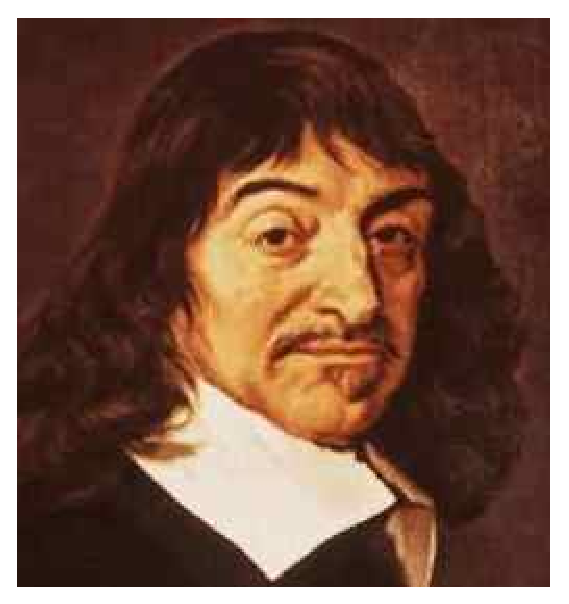
\includegraphics[width=6cm]{descartes.eps}\\
        {\footnotesize http
://files.db3nf.com/pictures/authors/descartes.jpg}
    \end{center}

1006-- Which mathematician was the first to study meteorology?

a$)$ Albert Einstein \\
b$)$ Augustin Louis Cauchy \\
c$)$ Ren\'e Descartes \\
d$)$ Sim\'eon Denis Poisson\\

Answer : c$)$\\

Feedback : \\
Ren\'e Descartes was the first one to study meteorology.
The answer is c$)$.\\

        \begin{center}
        Ren\'e Descartes\\
    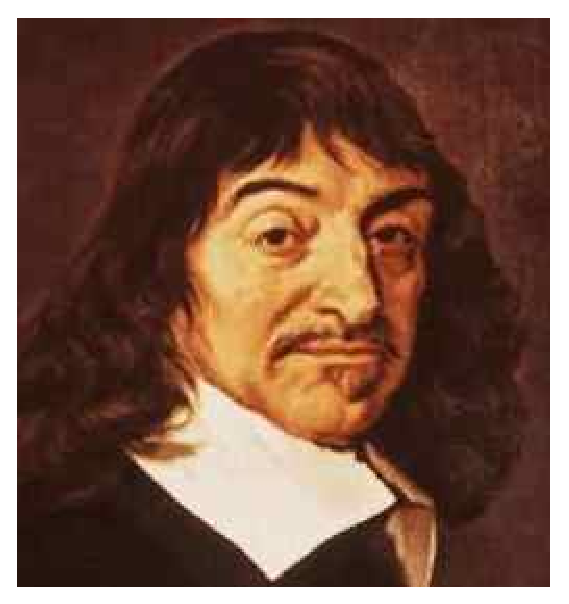
\includegraphics[width=6cm]{descartes.eps}\\
        {\footnotesize http
://files.db3nf.com/pictures/authors/descartes.jpg}
    \end{center}

1007-- How do we call the curve defined by the path of a point 
on the edge of circular wheel as the wheel rolls along a straight line?

a$)$ The {\sl cycloid} \\
b$)$ The {\sl straight} \\
c$)$ The {\sl Cartesian folium} \\
d$)$ The {\sl hyperbola}\\

Answer : a$)$\\

Feedback : \\
This figure is the cycloid.
The answer is a$)$.\\

        \begin{center}
       Cyclo\"ide \\
    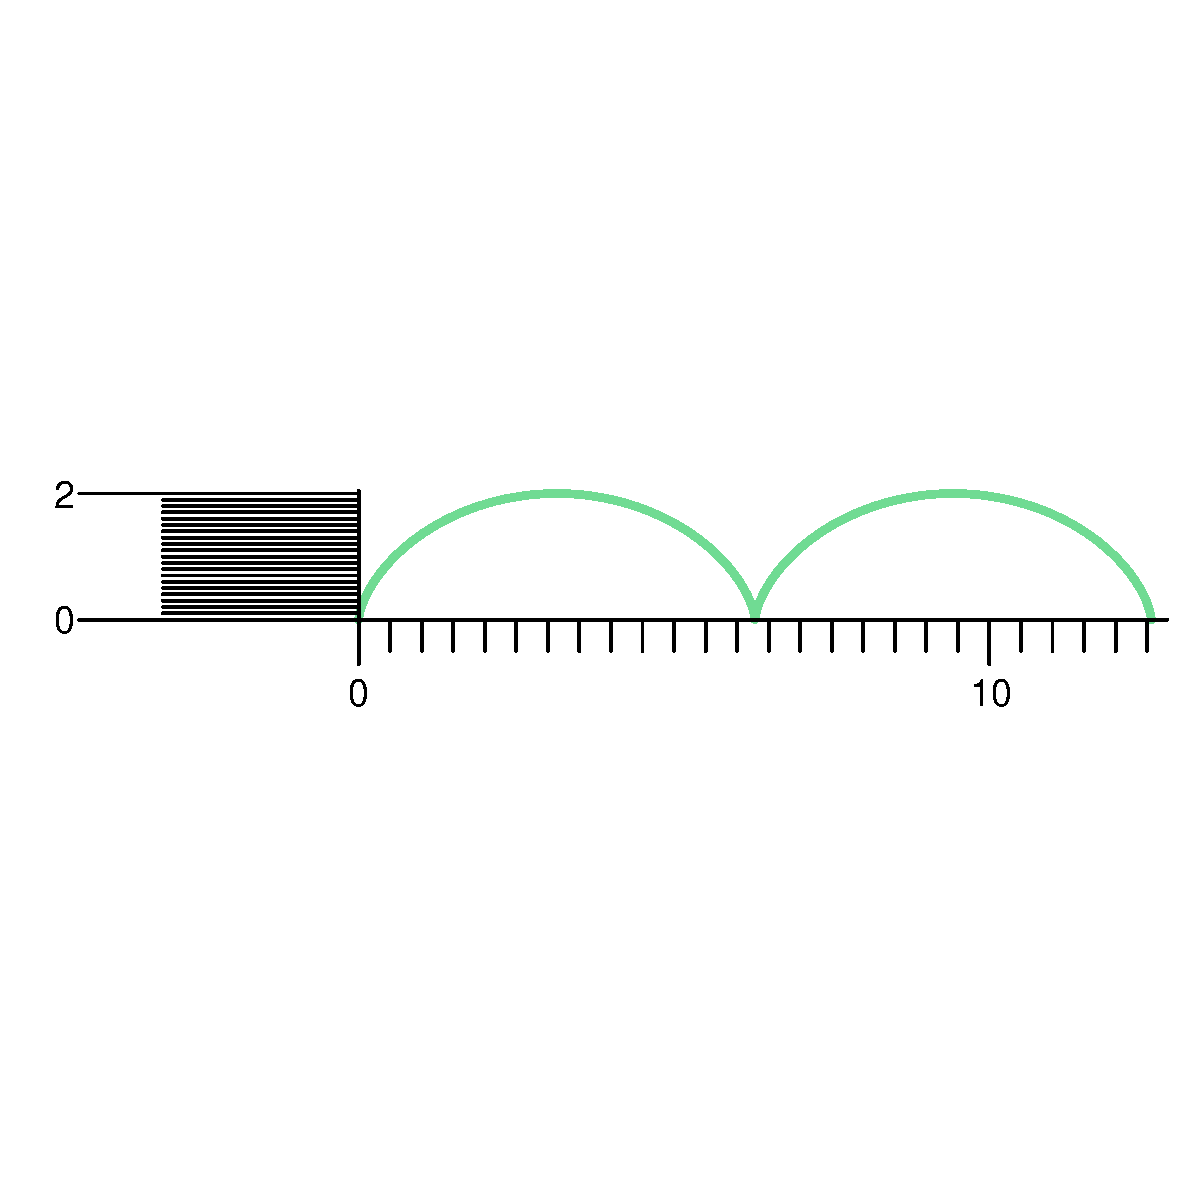
\includegraphics[width=6cm]{cycloide.eps}\\
    \end{center}

1008-- Which letters of the alphabet did Ren\'e Descartes usually use to refer to constants?

a$)$ The letters starting from $i$ \\
b$)$ The letters starting from $p$ \\
c$)$ The last letters \\
d$)$ The Ferst letters \\

Answer : d$)$\\

Feedback : \\
Descartes usually used the first letters of the alphabet to 
refer to constants. He also used the last letters of the 
alphabet to refer to unknown variables. It is to Descartes 
that we owe this custom.
The answer is d$)$.\\

        \begin{center}
        Ren\'e Descartes\\
    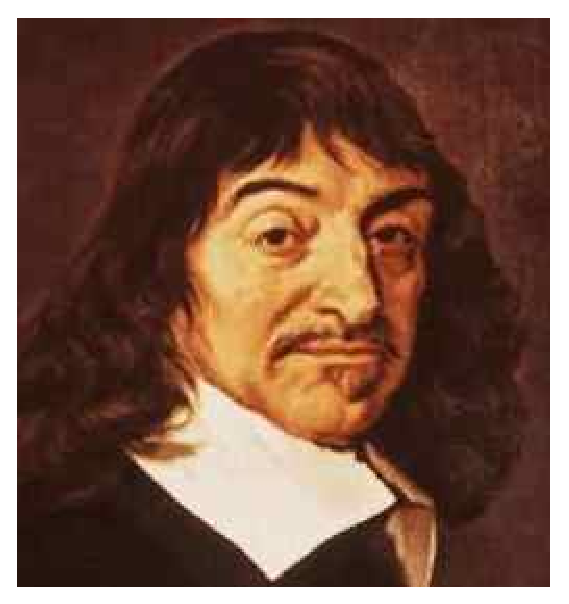
\includegraphics[width=6cm]{descartes.eps}\\
        {\footnotesize http
://files.db3nf.com/pictures/authors/descartes.jpg}
    \end{center}

1009-- Until what time did Descarte have the habit of staying in bed?

a$)$ 5 am \\
b$)$ 11 am \\
c$)$ 2 pm \\
d$)$ 5 pm\\

Answer : b$)$\\

Feedback :\\
Because of his health, Descartes took the habit of staying in 
bed until 11 am at an early age, which he did until the last 
year of his life. In fact, in 1649, he was induced by the Queen 
of Sweden to go to Stockholm in order to give her geometry 
lessons. However, because she preferred to draw tangents at 5 am, 
Descartes caught a cold and died of pneumonia.
   
The answer is b$)$.\\

        \begin{center}
        Ren\'e Descartes\\
    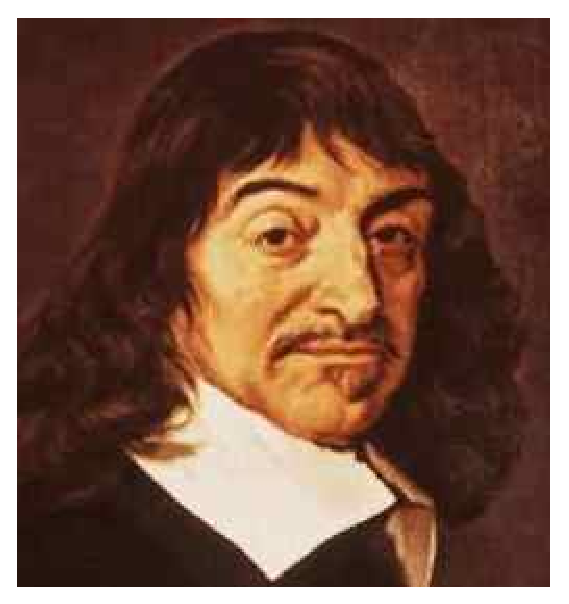
\includegraphics[width=6cm]{descartes.eps}\\
        {\footnotesize http
://files.db3nf.com/pictures/authors/descartes.jpg}
    \end{center}

1010-- For whom did Ren\'e Descartes have to get up at 5 am?

a$)$ His mother \\
b$)$ The Queen of Norway \\
c$)$ The Queen of Sweden \\
d$)$ His sister\\

Answer : c$)$\\

Feedback : \\
It is the Queen of Sweden, who enjoyed his geometry lessons. 
Descartes had poor health and died of pneumonia during that year.

The answer is c$)$.\\

        \begin{center}
        Ren\'e Descartes\\
    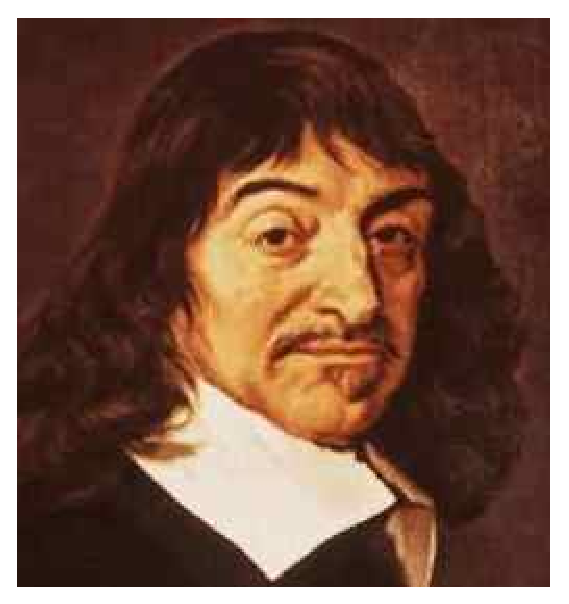
\includegraphics[width=6cm]{descartes.eps}\\
        {\footnotesize http
://files.db3nf.com/pictures/authors/descartes.jpg}
    \end{center}

1011-- Where did Ren\'e Descartes give his geometry classes during the last year of his life?

a$)$ Berlin \\
b$)$ New York \\
c$)$ Rome \\
d$)$ Stockholm\\

Answer : d$)$\\

Feedback :\\
It is Stockholm. Descartes was induced by the Queen of Sweden 
to go to Stockholm in order to give her geometry lessons. 
However, because she preferred \og to draw tangents\fg\ at 5 am, 
Descartes caught a cold and died of pneumonia.
The answer is d$)$.\\

        \begin{center}
        Ren\'e Descartes\\
    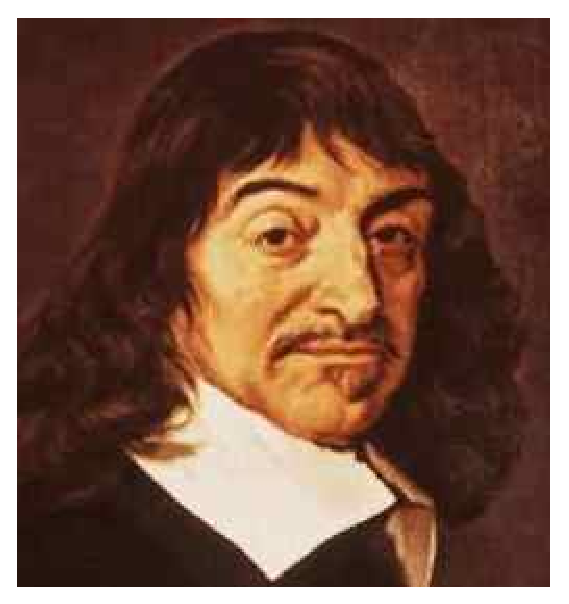
\includegraphics[width=6cm]{descartes.eps}\\
        {\footnotesize http
://files.db3nf.com/pictures/authors/descartes.jpg}
    \end{center}

        \begin{center}
        Stockholm\\
    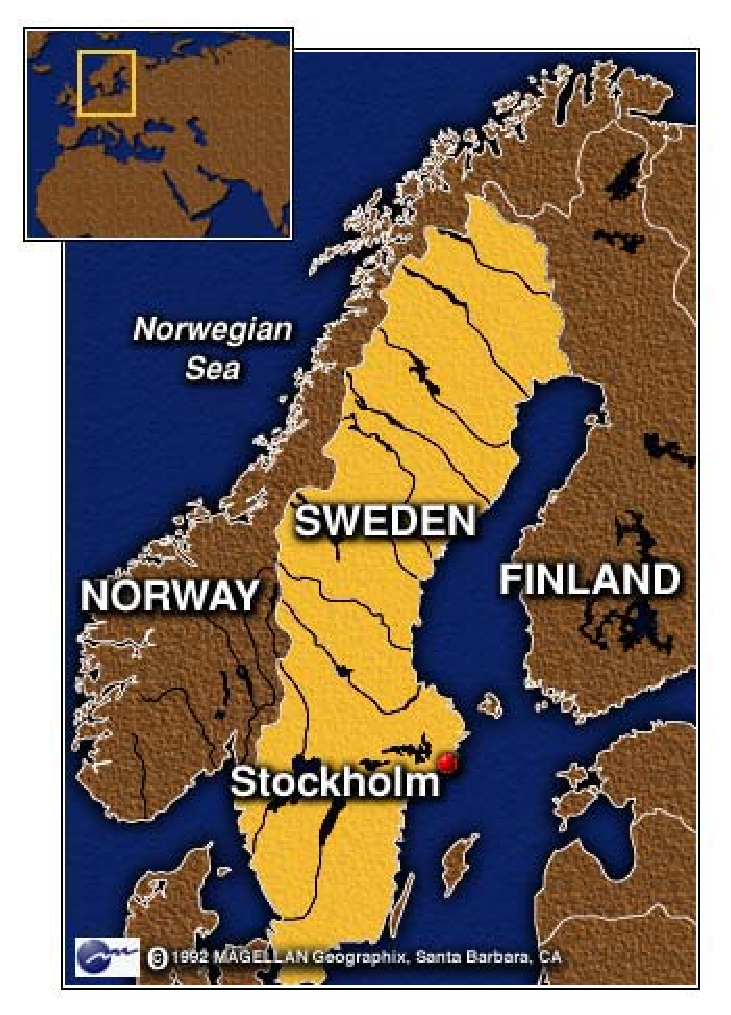
\includegraphics[width=6cm]{stosto.eps}\\
    \end{center}

1012-- How did Ren\'e Descartes die?

a$)$ pneumonia \\
b$)$ poisonned \\
c$)$ shot \\
d$)$ drowned\\

Answer : a$)$\\

Feedback :\\
Ren\'e Descartes died of pneumonia. Because of his health, 
Descartes took the habit of staying in bed until 11 am at an 
early age, which he did until the last year of his life. In 
fact, in 1649, he was induced by the Queen of Sweden to go to 
Stockholm in order to give her geometry lessons. However, 
because she preferred to draw tangents at 5 am, Descartes caught 
a cold and died of pneumonia.

The answer is a$)$.\\

        \begin{center}
        Ren\'e Descartes\\
    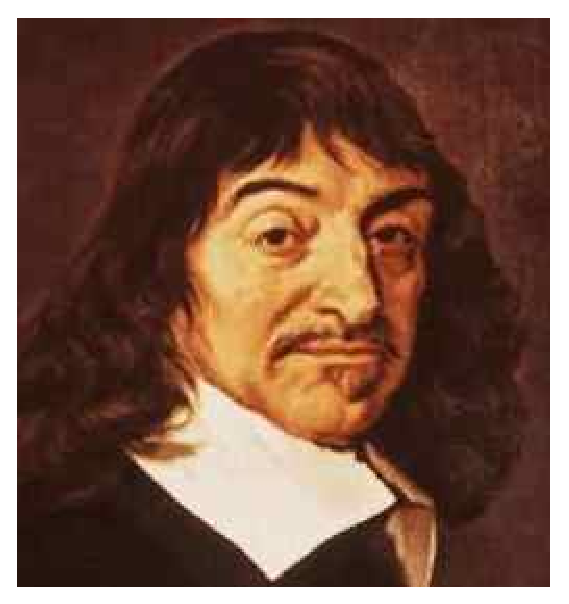
\includegraphics[width=6cm]{descartes.eps}\\
        {\footnotesize http
://files.db3nf.com/pictures/authors/descartes.jpg}
    \end{center}

1013-- Who demonstrated that the volume of a cone is one third of the volume of the cylinder that contains it?

a$)$ Bonaventura Cavalieri \\
b$)$ Michael Faraday \\
c$)$ Platon \\
d$)$ William Rowan Hamilton\\

Answer : a$)$\\

Feedback : \\
It is Bonaventura Cavalieri.
The answer is a$)$.\\

        \begin{center}
        Bonaventura Cavalieri\\
    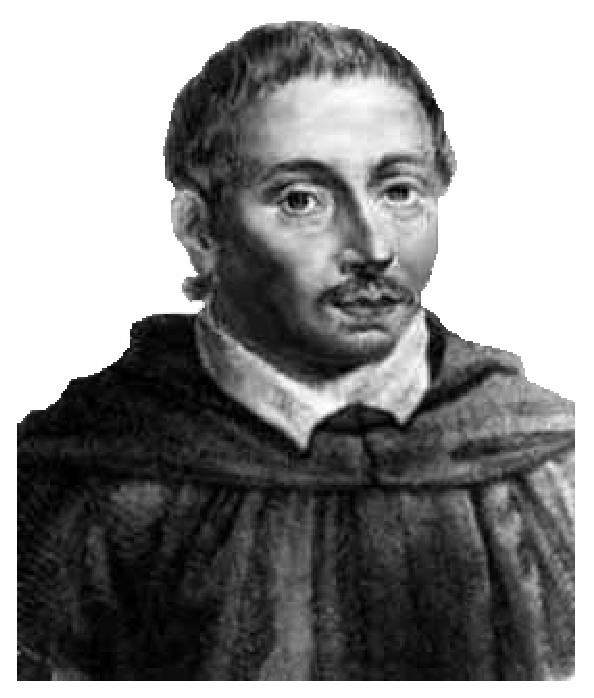
\includegraphics[width=6cm]{Cavalieri.eps}\\
        {\footnotesize http
://filebox.vt.edu/users/rboehrin/Cavalieri/Artwork/Cavalieri.gif}
    \end{center}

1014 * -- Who attained, in 1635, a formula for
$S_k(n)=1^k\,+\,2^k\,+\,\ldots\,+\,n^k$ valid when
$k=1,2,\ldots,9$ ?

a$)$ Alfred Nobel \\
b$)$ Bonaventura Cavalieri \\
c$)$ George Boole \\
d$)$ Pierre-Laurent Wantzel\\

Answer : b$)$\\

Feedback : \\
It is Bonaventura Cavalieri.
The answer is b$)$.\\

        \begin{center}
        Bonaventura Cavalieri\\
    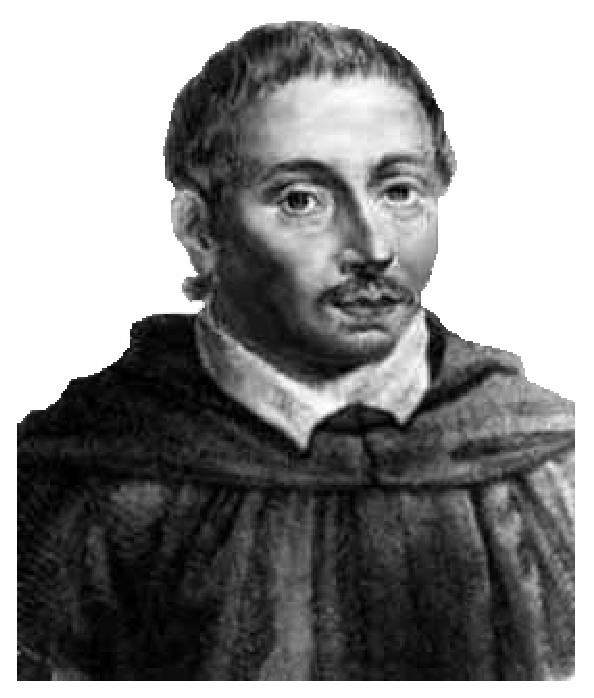
\includegraphics[width=6cm]{Cavalieri.eps}\\
        {\footnotesize http
://filebox.vt.edu/users/rboehrin/Cavalieri/Artwork/Cavalieri.gif}
    \end{center}

1015 * -- {\sl \'Given an integer $n>2$, the equation
$x^n\,+\,y^n=z^n$ does not have a solution for positive 
integers $x$, $y$ et $z$}. How is this theorem called?

a$)$  {\sl Fermat's last theorem} \\
b$)$ 	{\sl Riemann's hypothesis} \\
c$)$  {\sl Fermat's little theorem} \\
d$)$  {\sl Faith theorem}\\

Answer : a$)$\\

Feedback : \\
This theorem is called {\sl Fermat's last theorem}. Even if 
Fermat did not succeed on demonstrating this result, we still 
call it \og theorem \fg\ for historical reasons. In 1994, a 
British mathematician, Andrew Wiles, managed to provide a 
demonstration of Fermat's theorem.
The answer is a$)$.\\

        \begin{center}
        Fermat\\
    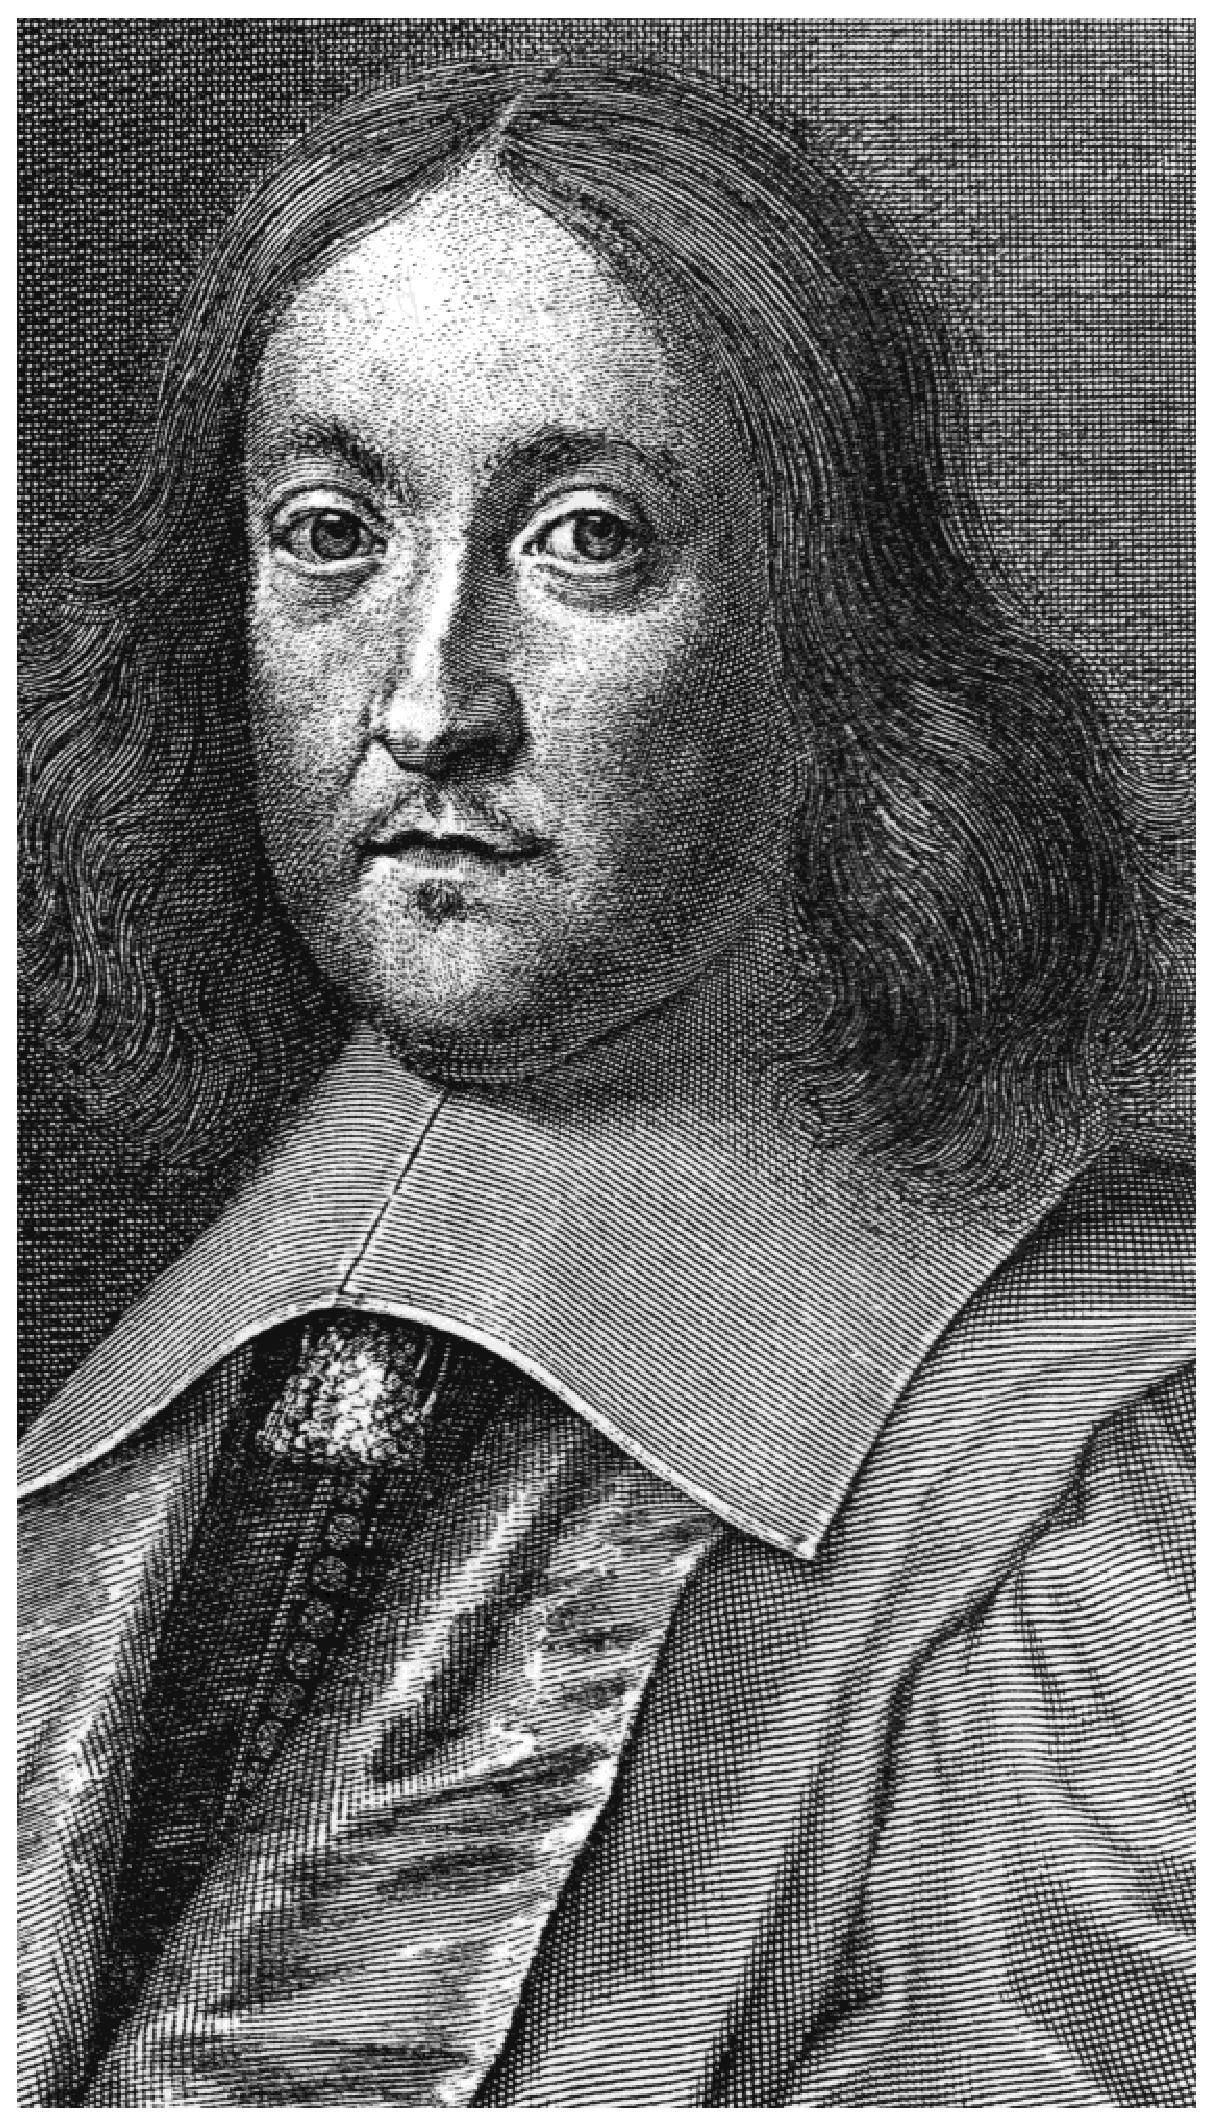
\includegraphics[width=6cm]{fermat.eps}\\
        {\footnotesize http
://www.york.ac.uk/depts/maths/histstat/people/fermat.gif}
    \end{center}

        \begin{center}
        Andrew Wiles\\
    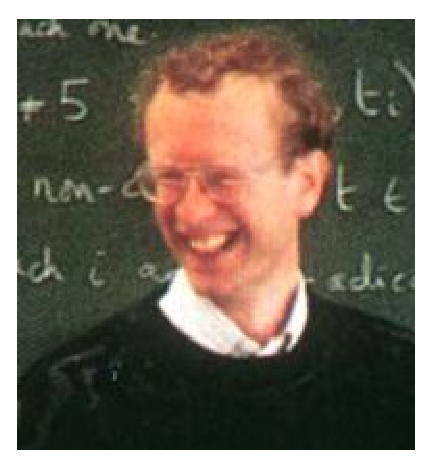
\includegraphics[width=6cm]{wiles.eps}\\
        {\footnotesize http
://www.pims.math.ca/education/2000/bus00/cubes/wiles.jpg}
    \end{center}

1016 * -- Let $A$, $B$ and $C$ be integers. If the greatest 
common divisor of $A$ and $B$ is $1$, then $A$ and $B$ are 
said to be coprime. If $C$ divides $A\,-\,B$, then we will 
write $A\equiv B\,(\mathrm{mod}\,C)$. Which of the following 
four results is called  {\sl Fermat's little theorem} and is 
at the basis of the most enhanced encoding methods.

a$)$ {\sl Given coprime integers $a$ et $b$ then $b^{a\,-\,1}\equiv1\,(\mathrm{mod}\,a)$.} \\
b$)$ {\sl \'Given a prime number $p$ and coprime integers $a$ and $p$, then
$a^{p\,-\,1}\equiv1\,(\mathrm{mod}\,p)$.} \\
c$)$ {\sl \'Given a prime number $p$ and coprime integers $a$ and $p$, alors
$p^{a\,-\,1}\equiv1\,(\mathrm{mod}\,a)$.} \\
d$)$ {\sl All odd numbers are prime.}\\

Answer : b$)$\\

Feedback : \\
The result is: {\sl \'Given a prime number $p$ and coprime integers $a$ and $p$, then
$a^{p\,-\,1}\equiv1\,(\mathrm{mod}\,p)$.}
The answer is b$)$.\\

1017-- The {\sl Fermat numbers} are numbers of type $F_n=2^{2^n}\,+\,1, n=0,1,2,\ldots$ For example, for $n=2$,
$17=2^{2^2}\,+\,1$ is a Fermet number. What is the greatest known Fermat prime?

a$)$ $1000$ \\
b$)$ $2^{2^4}\,+\,1$ \\
c$)$ $2^{2^5}\,+\,1$ \\
d$)$ $2^{2^6}\,+\,1$\\

Answer : b$)$\\

Feedback : \\
The greatest known Fermat prime is $2^{2^4}\,+\,1$.
Fermat believed that each of these numbers were prime.
He was right for $F_0=3$, $F_1=5$, $F_2=17$, $F_3=257$ and
$F_4=65\,537$. Euler demonstrated that his statement in general was false because
$2^{2^5}\,+\,1=2^{32}\,+\,1=4\,294\,967\,297=641\cdot6\,700\,417$.
Today,we know that the numbers $F_5,F_6,\ldots,F_{24}$ are all composite numbers.

The answer is b$)$.\\

1018-- Some numbers can be written as sums of two squares. For example, 
$13=4\,+\,9=2^2\,+\,3^2$ is one of those numbers. Which of the 
following numbers can be written as the sum of two squares?

a$)$ $3$ \\
b$)$ $3^2\,\times\,7=63$\\
c$)$ $3^2\,\times\,7^2=441$ \\
d$)$ $3^2\,\times\,11^3=11\,979$\\

Answer : c$)$\\

Feedback : \\
A result attributed to Fermat has to be used: {\sl an integer $n$ can
be represented as the sum of two squares if and only if each of its prime 
factors of type $4k\,+\,3$ appears with an even exponent on prime 
factorization of $n$.} However, the three prime numbers of type $4k\,+\,3$ 
are $3=0\,+\,3=4(0)\,+\,3$, $7=4\,+\,3=4(1)\,+\,3$ and $11=8\,+\,3=4(2)\,+\,3$. 
Only $441$ has even exponents on prime factors of type $4k\,+\,3$ of its prime 
factorization.

The answer is c$)$.\\

1019-- Who is the cofounder, with Descartes, of analytical geometry?

a$)$ Blaise Pascal \\
b$)$ Charles Hermite \\
c$)$ Georg Bernhard Riemann \\
d$)$ Pierre de Fermat\\

Answer : d$)$\\

Feedback : \\
Pierre de Fermat is cofounder of analytical geometry.
The answer is d$)$.\\

        \begin{center}
        Pierre de Fermat\\
    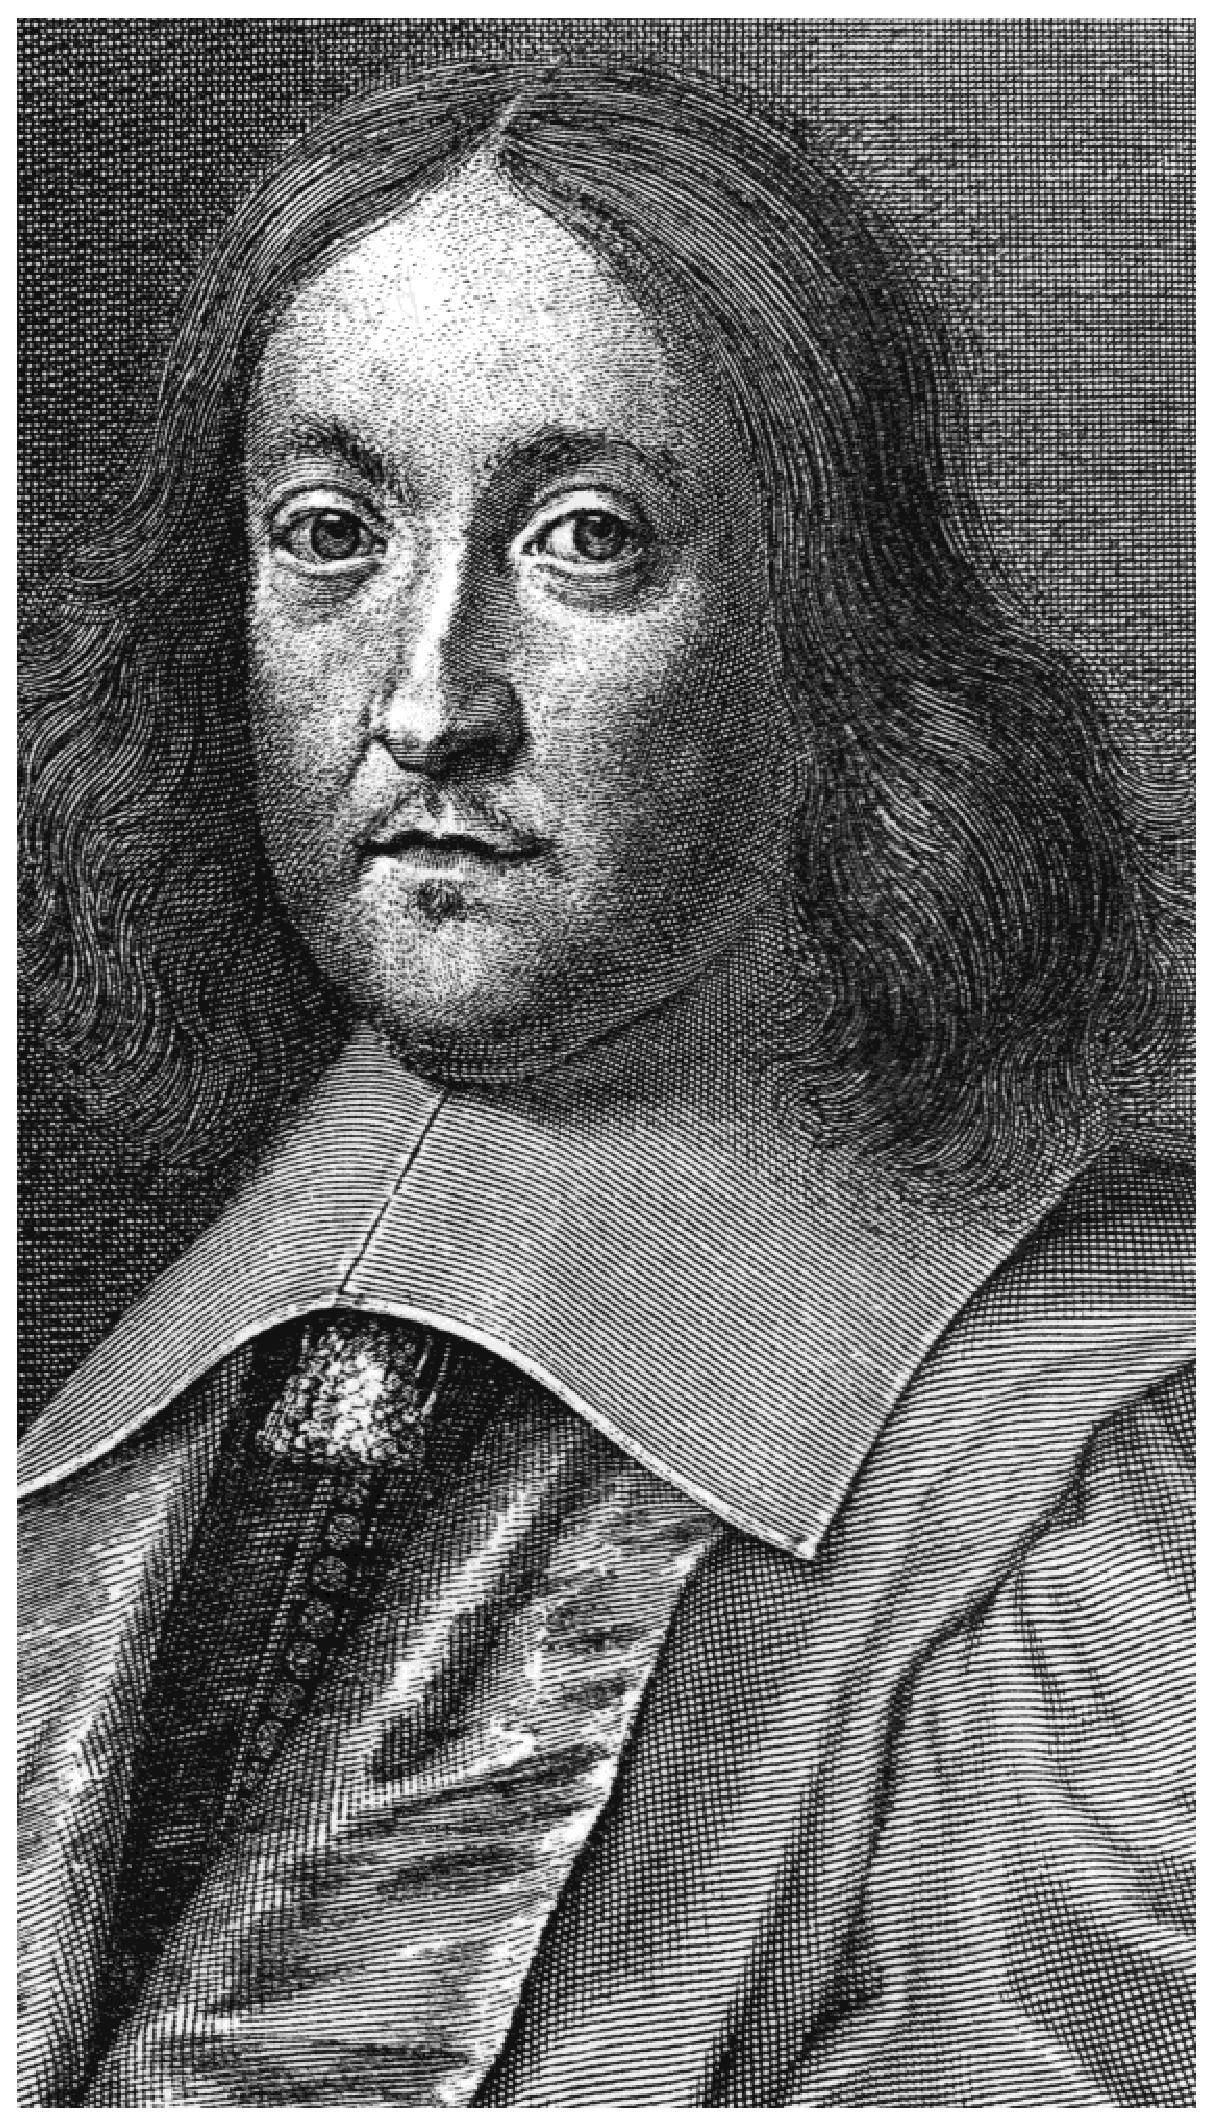
\includegraphics[width=6cm]{fermat.eps}\\
        {\footnotesize http
://www.york.ac.uk/depts/maths/histstat/people/fermat.gif}
    \end{center}

1020-- Who is the cofounder, with Pascal, of the probability theory?

a$)$ Franz Mertens \\
b$)$ Hermann Schwarz \\
c$)$ Louis Pasteur \\
d$)$ Pierre de Fermat\\

Answer : d$)$\\

Feedback : \\
Pierre de Fermat is cofounder of the probability theory.
The answer is d$)$.\\

        \begin{center}
        Pierre de Fermat\\
    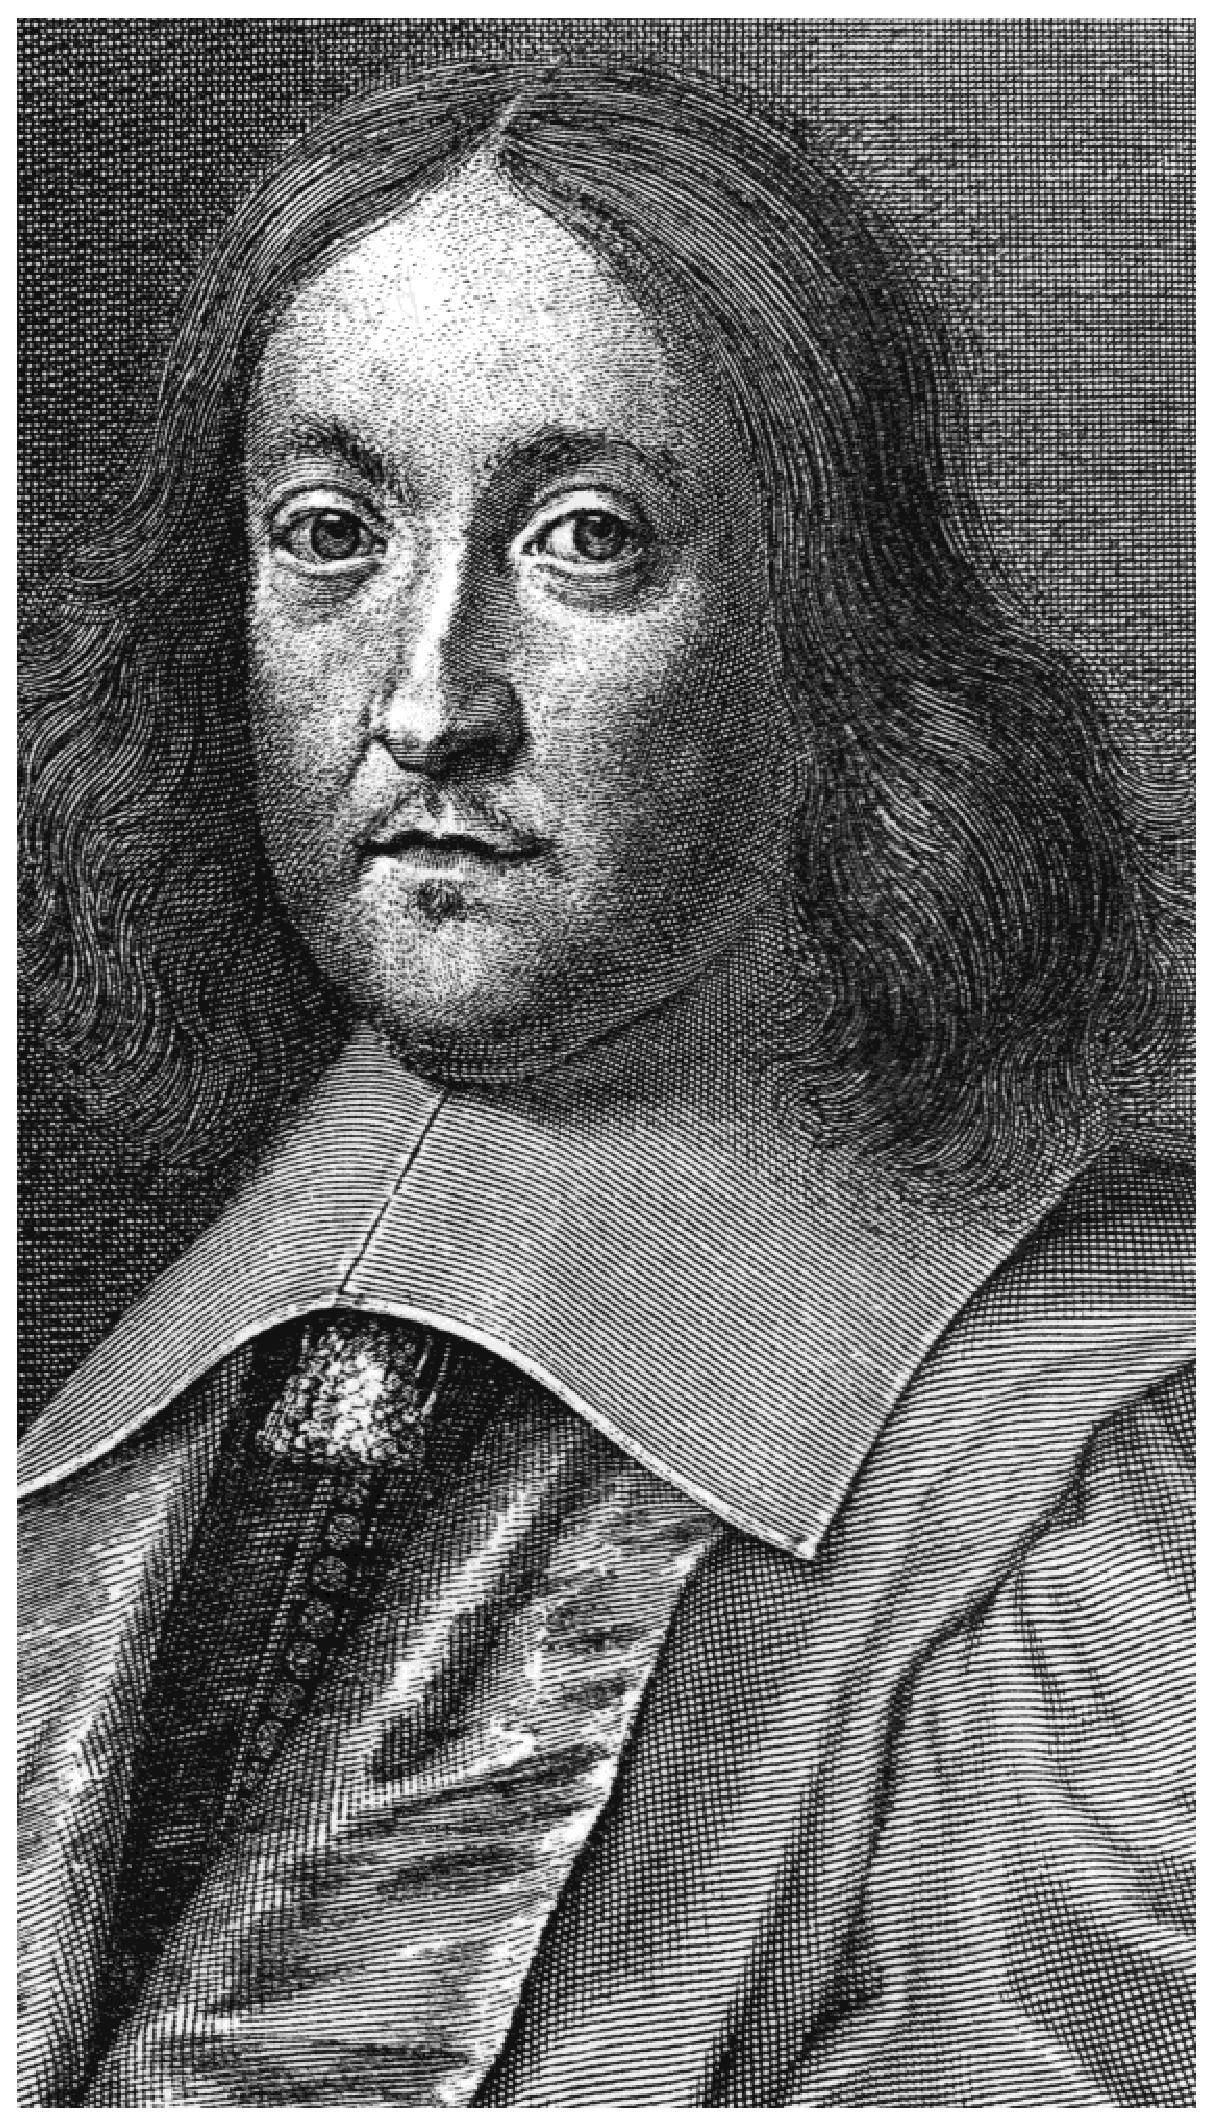
\includegraphics[width=6cm]{fermat.eps}\\
        {\footnotesize http
://www.york.ac.uk/depts/maths/histstat/people/fermat.gif}
    \end{center}

1021 * -- Where does Pierre de Fermat mentions for the first time his 
{method of infinite descent}?

a$)$ In personal notes that show that the equation $x^4\,+\,y^4=z^4$
 has no solution for integers $x,y\,$ and $\,z$ non nulls. \\
b$)$ In the book {\sl Sophie's world} \\
c$)$ In the work {\sl La G\'eom\'etrie} \\
d$)$ In a letter to Huygens\\

Answer : d$)$\\

Feedback : \\
It's in a letter to Huygens that he uses this method to demonstrate 
that no numbers of type $3k\,-\,1$ is of type $x^2\,+\,3y^2$, which
is literally useless since the equation $x^2\,+\,3y^2=3k\,-\,1$ has 
obviously no solutions modulo $3$, because $x^2\not
\equiv-1\,(\mathrm{mod}\,3)$.
The answer is d$)$.\\

        \begin{center}
        Pierre de Fermat\\
    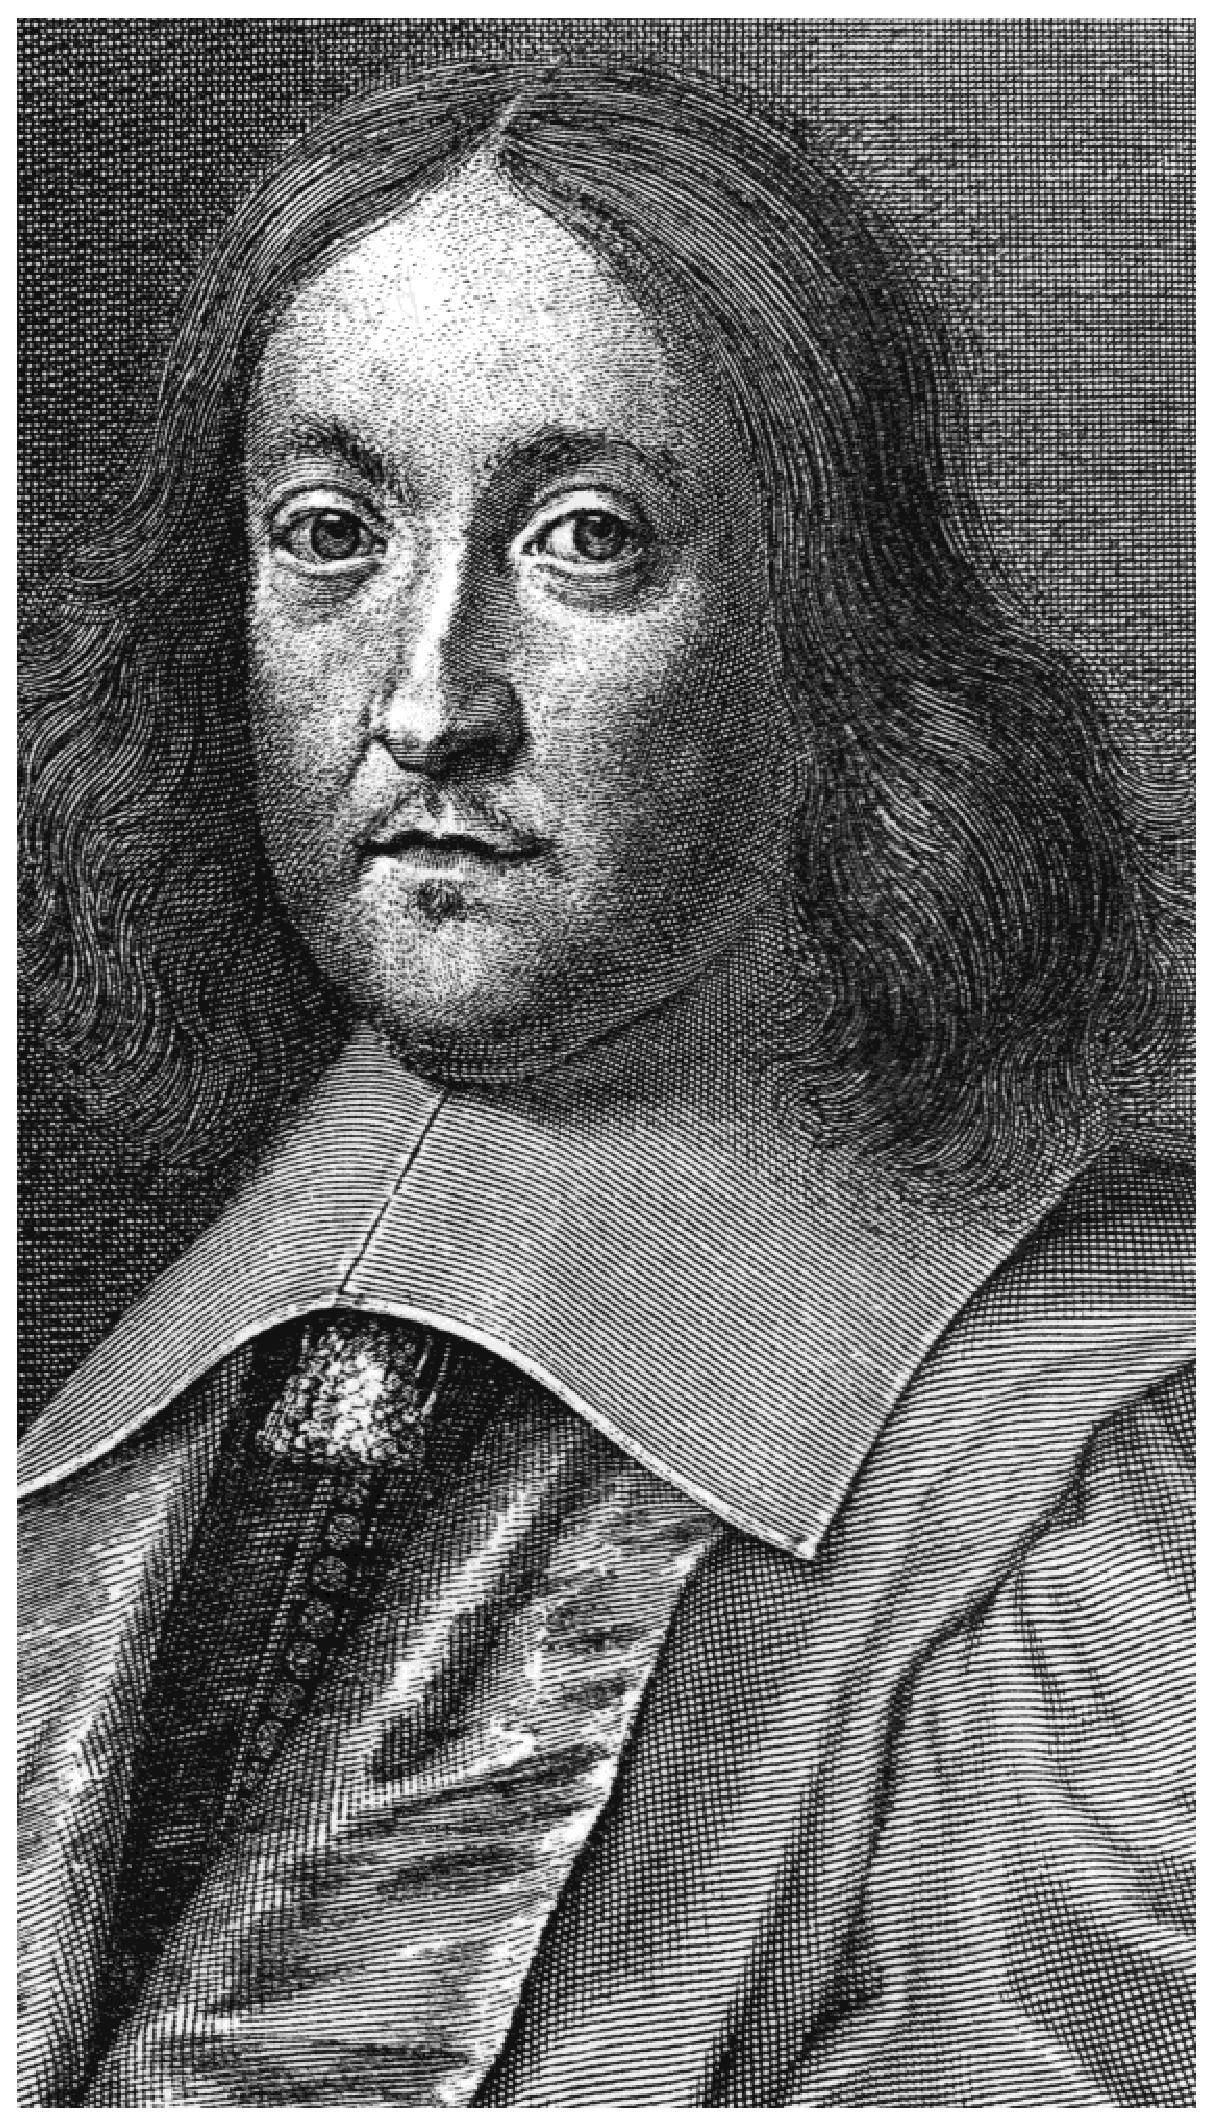
\includegraphics[width=6cm]{fermat.eps}\\
        {\footnotesize http
://www.york.ac.uk/depts/maths/histstat/people/fermat.gif}
    \end{center}

        \begin{center}
        Christian Huygens\\
    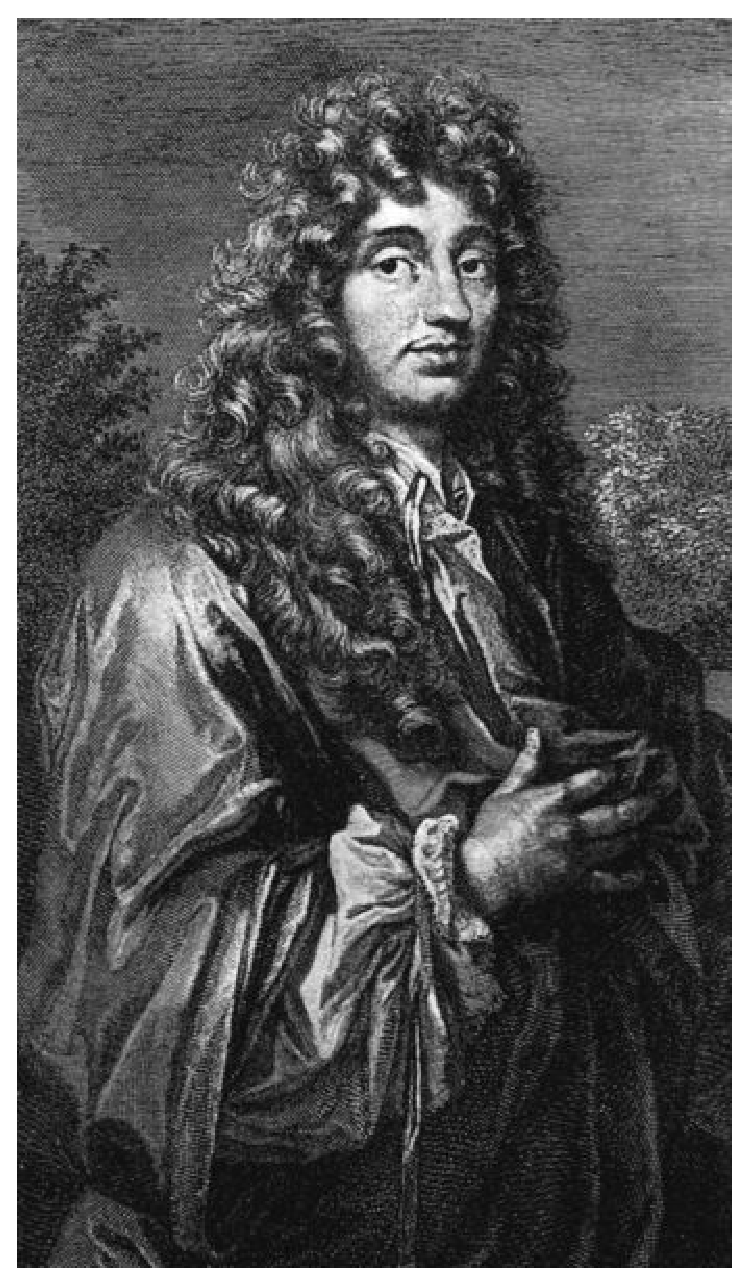
\includegraphics[width=6cm]{huygens.eps}\\
        {\footnotesize http
://www.th.physik.uni-frankfurt.de/$\sim$jr/gif/phys/huygens.jpg}
    \end{center}

1022 * -- Let $f$ be a function as well as $a$, $b$ and $c$ be real numbers
like $c\in(a,b)$ and $(a,b)$ is included in the domain of $f$. 
If we have $f(c)>f(t)$ for all $t\in(a,b)$ like
$t\not=c$, then we will say that $c$ is a maxima of $f$. It is the same
if we have $f(c)<f(t)$ for all $t\in(a,b)$ like $t\not=c$, then we will say that
$c$ is a minima of $f$. Which seventeenth-century mathematician found a method to
determine the maxima and minima of a function?

a$)$ David Hilbert \\
b$)$ Henri Poincar\'e \\
c$)$ Lord Kelvin \\
d$)$ Pierre de Fermat \\

Answer : d$)$\\

Feedback : \\
It is Pierre de Fermat.
The answer is d$)$.\\

        \begin{center}
        Pierre de Fermat\\
    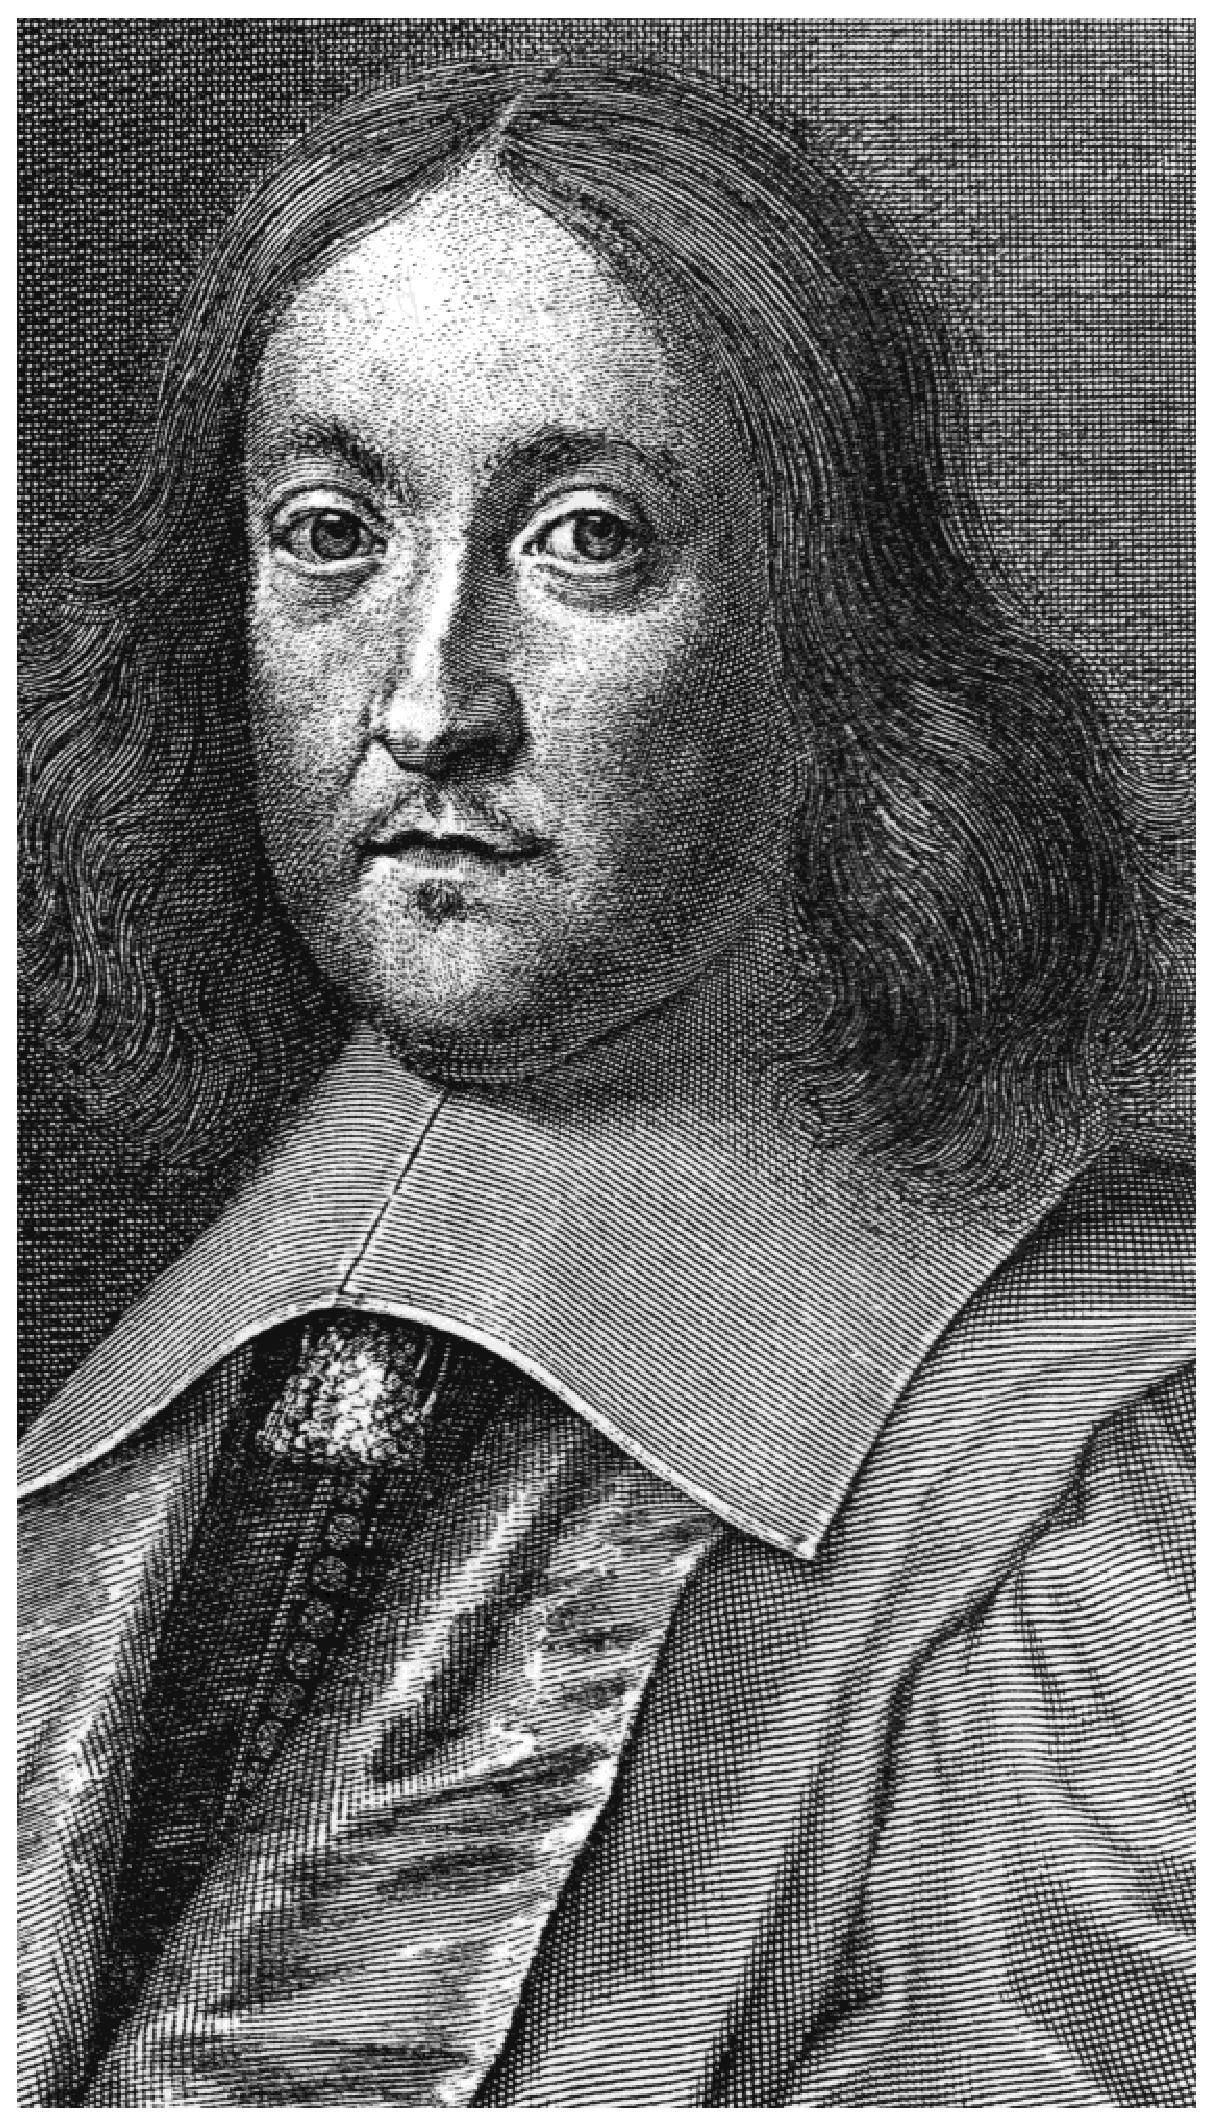
\includegraphics[width=6cm]{fermat.eps}\\
        {\footnotesize http
://www.york.ac.uk/depts/maths/histstat/people/fermat.gif}
    \end{center}

1023-- Which mathematician was Pierre de Fermat always at odds with?

a$)$ Bertrand Russell \\
b$)$ Jacques Hadamard \\
c$)$ Pythagore \\
d$)$ Ren\'e Descartes\\

Answer : d$)$\\

Feedback : \\
Pierre de Fermat was constantly at odds with Ren\'e
Descartes. The answer is d$)$.

        \begin{center}
        Pierre de Fermat\\
    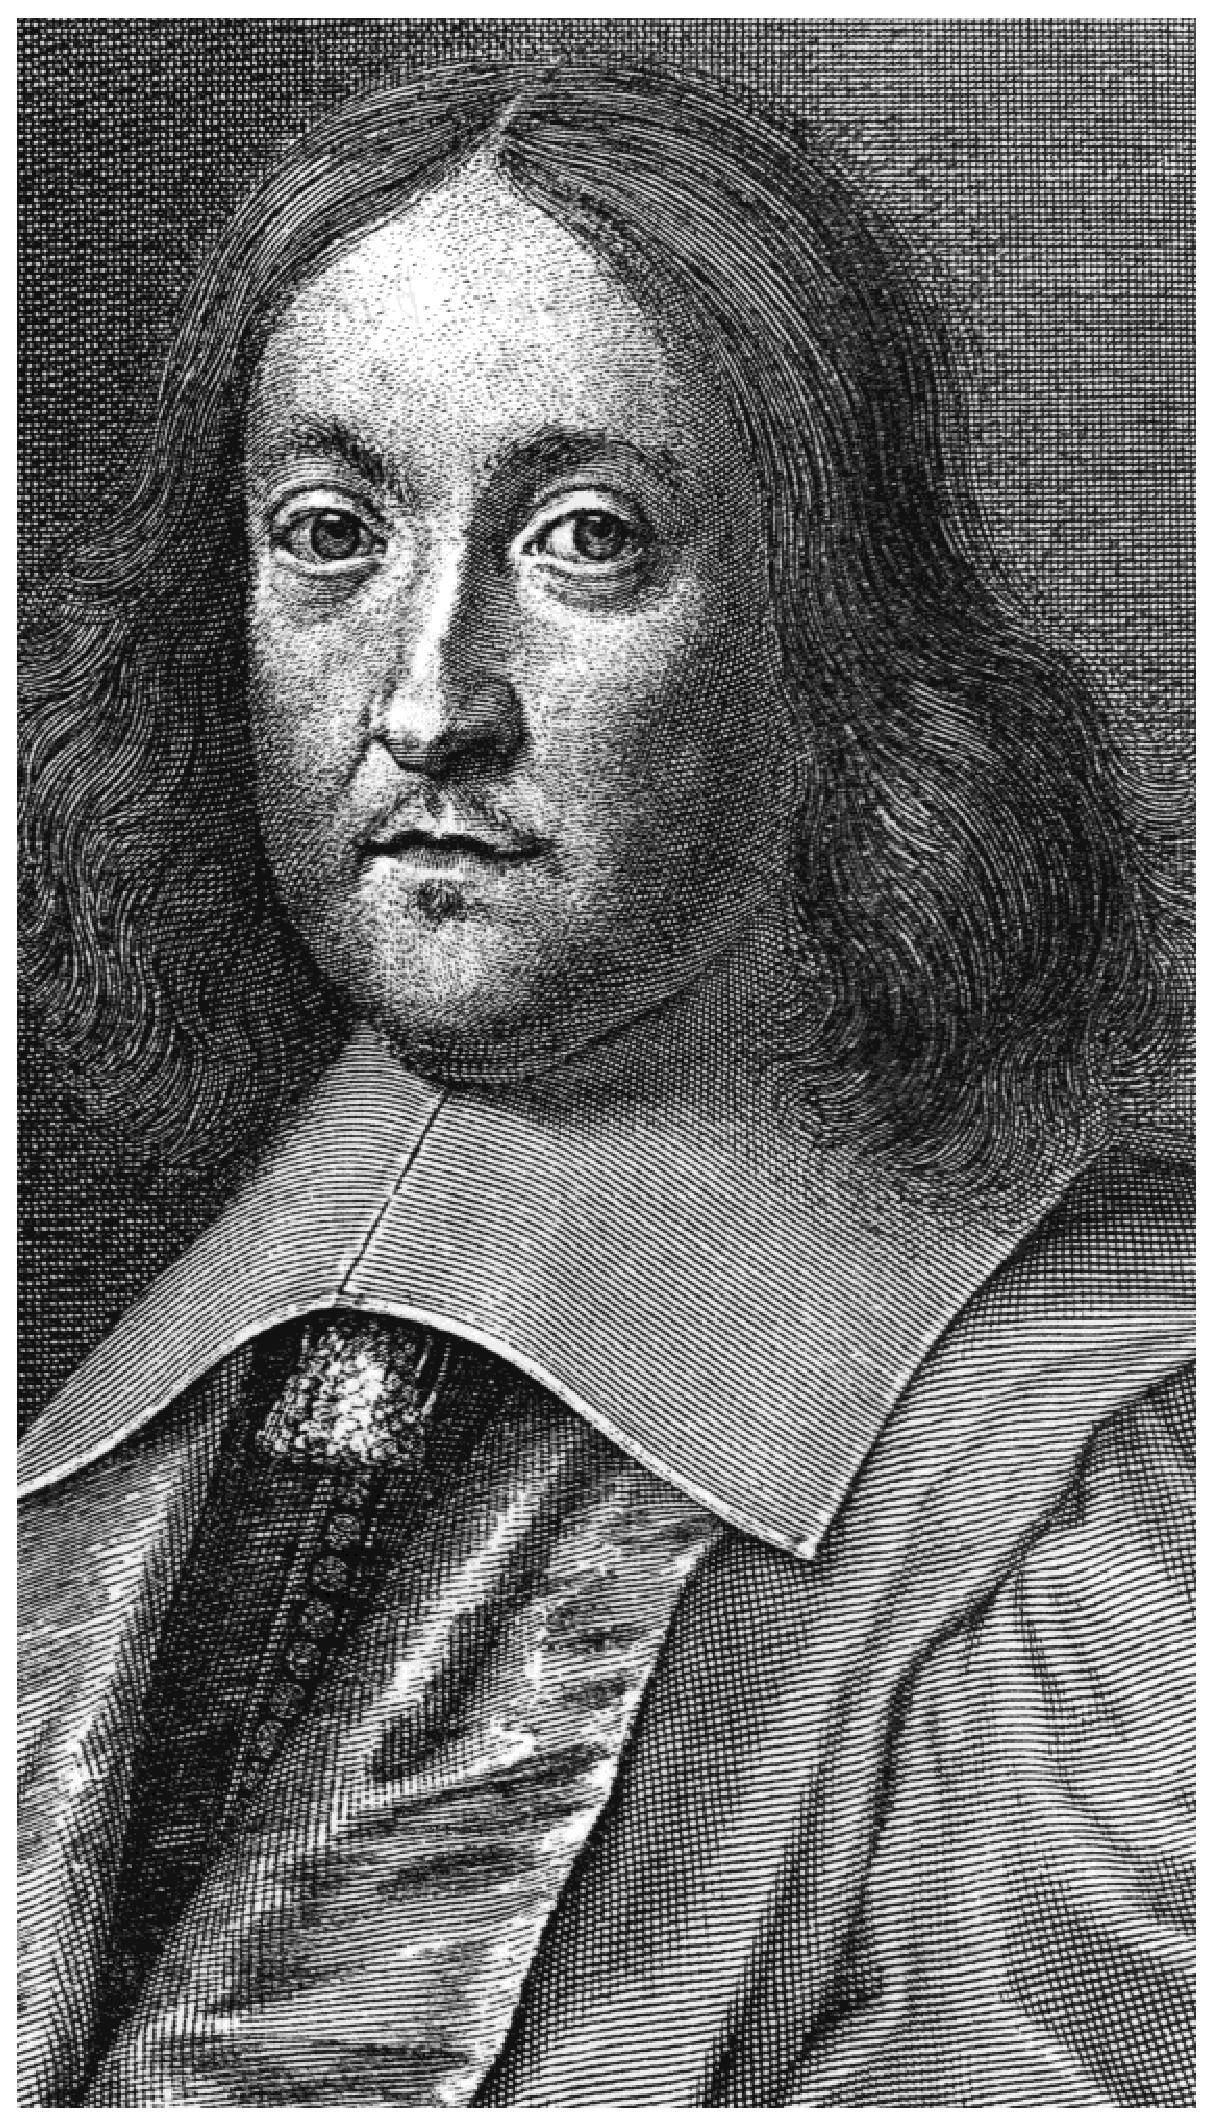
\includegraphics[width=6cm]{fermat.eps}\\
        {\footnotesize http
://www.york.ac.uk/depts/maths/histstat/people/fermat.gif}
    \end{center}

        \begin{center}
        Ren\'e Descartes\\
    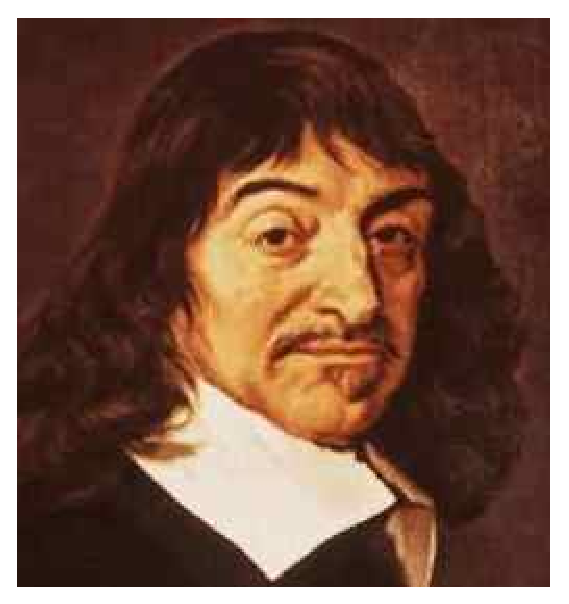
\includegraphics[width=6cm]{descartes.eps}\\
        {\footnotesize http
://files.db3nf.com/pictures/authors/descartes.jpg}
    \end{center}


1024 * -- {\sl If $f$ is a derivative on interval
$[a,b]$ and if $f(a)=f(b)=0$, then there exists a number $x_0\in[a,b]$
like $f'(x_0)=0$}. To whom do we owe this theorem?

a$)$ Galileo Galil\'ee \\
b$)$ Gilles Personne de Roberval \\
c$)$ Michel Rolle \\
d$)$ William Shakespeare\\

Answer : c$)$\\

Feedback : \\
We owe this theorem to Michel Rolle.
The answer is c$)$.\\


1025 * -- Which number did Pierre de Fermat factorize with
Fermat's factorization test?

a$)$ $29$ \\
b$)$ $146$ \\
c$)$ $2^{61}\,-\,1$ \\
d$)$ $2\,027\,651\,281$\\

Answer : d$)$\\

Feedback : \\
It is $2\,027\,651\,281$. Given an odd composite number $n$, 
this test consists of using the fact that there exists positive integers
$a$ and $b$ like $n=a^2\,-\,b^2$, in which case $n=(a\,-\,b)(a\,+\,b)$ delivers a factorization of $n$.
It is an efficient method if the integer $n$ has two relatively close divisors. In Fermat's example, 
he first calculated $[\sqrt{
2\,027\,651\,281}]=45\,029$. He started with
$a=45\,029\,+\,1=45\,030$; since
$45\,030^2\,-\,2\,027\,651\,281=49\,619$ is not a perfect square,
he went on to $a=45\,031$, which still doesn't give a perfect square, 
and so on and so forth, until he got to $a=45\,041$, which gives
$b=\sqrt{45\,041^2\,-\,2\,027\,651\,281}=\sqrt{1\,040\,400}=1020$.
Then he could conclude that
$$n=2\,027\,651\,281=45\,041^2\,-\,1020^2=(45\,041\,-\,1020)(45\,041\,+\,1020)=44\,021\cdot46\,061.$$
The answer is d$)$.\\

1026-- In which country were Ren\'e Descartes (1596-1650), Pierre de Fermat
(1601-1665) and Gilles Personne de Roberval (1602-1675) born?

a$)$ Belgium  \\
b$)$ Congo \\
c$)$ France  \\
d$)$ Greece\\

Answer : c$)$\\

Feedback :\\
Ren\'e Descartes, Pierre de Fermat and Gilles Personne de Roberval
were born in France, like many other great mathematicians of their time, 
like Fran\c cois Vi\`ete, Marin
Mersenne, Blaise Pascal and many more. The answer is c$)$.

        \begin{center}
        France\\
    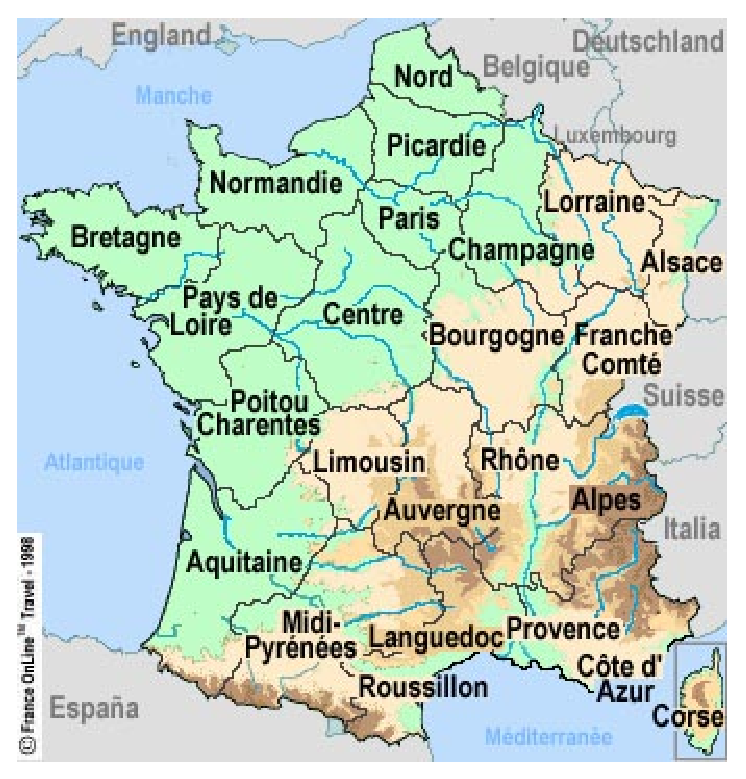
\includegraphics[width=6cm]{france.eps}\\
    \end{center}

1027-- Let $a,b\in\mathbb{R}$. Consider the surface 
defined by the function $\sin x$ for $x\in[a,b]$ and by the straight 
lines $x=a$, $x=b$ and $y=0$. Who was the first mathematician to
calculate this surface area?

a$)$ George David Birkhoff  \\
b$)$ Gilles Personne de Roberval \\
c$)$ John Forbes Nash  \\
d$)$ Thoralf Skolem\\

Answer : b$)$\\

Feedback :\\
Gilles Personne de Roberval was the first mathematician to calculate
the area of this surface. In more advanced terms, we
can say that he calculated the definite integral of $\sin x$.
The answer is b$)$.\\

1028 * -- The curve defined by the path of a point on the edge 
of circular wheel as the wheel rolls along a straight line 
is called a cycloid. Let $r$ be theradius of the circle that 
creates the cycloid. In 1634, Gilles Personne de Roberval 
found the value of the area under a cycloid arc, on the basis 
of $r$. Amongst the following, which one corresponds to this value?

a$)$ $r$  \\
b$)$ $100r$ \\
c$)$ $\pi r^2$  \\
d$)$ $3\pi r^2$ \\

Answer : d$)$\\

Feedback :\\
This value is $3\pi r^2$. In other terms, the area under a
cycloid arc is of three times the area of the circle that
creates it.
The answer is d$)$.\\

        \begin{center}
Cyclo\"ide        \\
    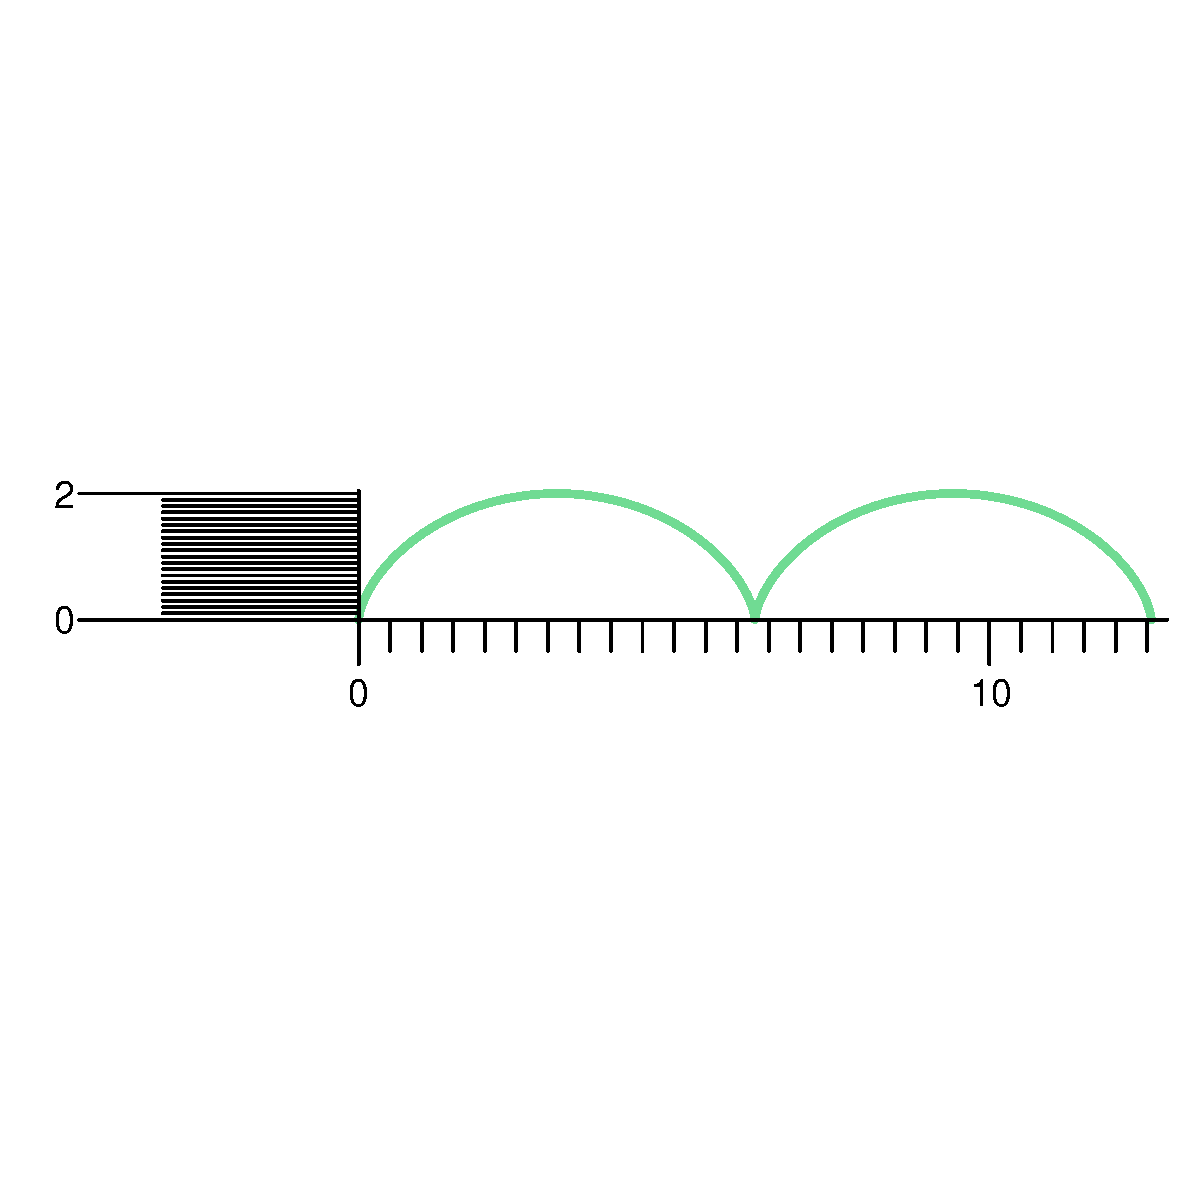
\includegraphics[width=6cm]{cycloide.eps}\\
    \end{center}

1029 * -- Just as circles, curves can have tangents
in one point. Let $f$ be a curve in the cartesian plane,
$(a,f(a))$ a point of this curve, and $d$ a straight line. We will say that
$d$ is a tangent of $f$ at point $(a,f(a))$ if $d(a)=f(a)$ and
there exists real numbers $b$ and $c$ like $a\in(b,c)$ and
$d\not=f$ for all $x\in(b,c)$ with$ x\not=a$. For example, for the
curve $f(x)=x^2$, we can easily verify that the straight line
$d(x)=0$ is tangent to $x^2$ at point $(0,0)$. Amongst the following,
which mathematician was one of the first, just like
Torricelli, Fermat et Descartes, to have calculated the tangent of
a curve in one point?

a$)$ Gilles Personne de Roberval  \\
b$)$ J\'anos von Neumann  \\
c$)$ Kurt G\"odel \\
d$)$ Max Planck\\

Answer : a$)$\\

Feedback :\\
Gilles Personne de Roberval was one the the first to calculate
the tangent of a curve in one point.
The answer is a$)$.\\

1030-- In what year did mathematician Gilles Personne de
Roberval invent the  {\sl Roberval's balance}, that is  the
platform scale?

a$)$ 334  \\
b$)$ 1669 \\
c$)$ 1902  \\
d$)$ 1988 \\

Answer : b$)$\\

Feedback :\\
Gilles Personne de Roberval invented this balance in 1669. The answer
is b$)$.\\

        \begin{center}
        {\sl Balance de Roberval}\\
    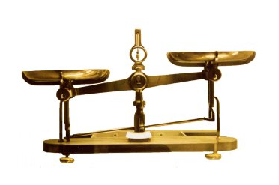
\includegraphics[width=6cm]{balbal.eps}\\
        {\footnotesize http
://visite.artsetmetiers.free.fr/images/instruments/balance\_roberval.jpg}
    \end{center}

1031-- During which cenury did these mathematicians live; Pierre de
Fermat, Gilles Personne de Roberval and Evangelista Torricelli?

a$)$ During the second century \\
b$)$ During the tenth century \\
c$)$ During the seventeenth century \\
d$)$ During the twentieth century

Answer : c$)$\\

Feedback : \\
These mathematicians lived during the seventeenth century. Pierre
de Fermat lived from 1601 to 1665,
Gilles Personne de Roberval from 1602 to 1675 and Evangelista Torricelli from
1608 to 1647. The answer is c$)$.\\

1032 * -- Who established, in 1643, that the volume created by making
the hyperbola $xy=k^2$ turn around the axis of $y$ between $y=a$ and
$y=\infty$ is finite and is in fact equal to the volume of a cylinder
of altitude $\frac{k^2}a$ and a radius equal to semidiameter
$k\sqrt2$ (which is the distance between the origin and point $(k,k)$ of the 
hyperbola)?

a$)$ Evangelista Torricelli \\
b$)$ John Forbes Nash \\
c$)$ Max Planck \\
d$)$ Paul Erd\H{o}s  \\

Answer : a$)$\\

Feedback : \\
It is d'Evangelista Torricelli. The answer is a$)$.\\

        \begin{center}
        Evangelista Torricelli\\
    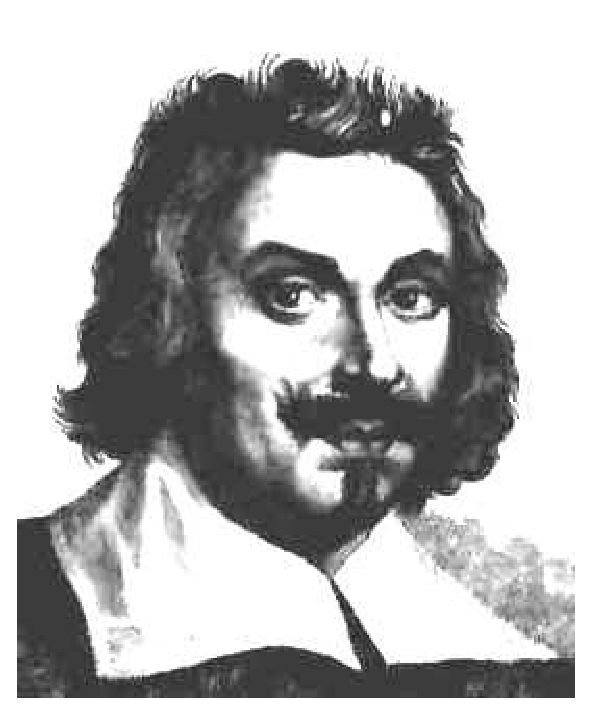
\includegraphics[width=6cm]{tortor.eps}\\
        {\footnotesize http ://www.whyy.org/tv12/franklinfacts/MAR1400.jpg}
    \end{center}

1033 * -- The curve defined by the path of a point on the edge of 
circular wheel as the wheel rolls along a straight line is called 
a cycloid. Let $r$ be theradius of the circle that creates the 
cycloid. In 1634, Gilles Personne de Roberval found the value 
of the area under a cycloid arc, on the basis of $r$. which 
mathematician ignored Roberval's result and arrived at the same 
result ten years later?

a$)$ Euclide d'Alexandrie \\
b$)$ Evangelista Torricelli \\
c$)$ Paul Cohen \\
d$)$ Yuri Vladimirovich Matijasevich\\

Answer : b$)$\\

Feedback : \\
It is Evangelista Torricelli. The answer is b$)$.\\

        \begin{center}
Cyclo\"ide\\
    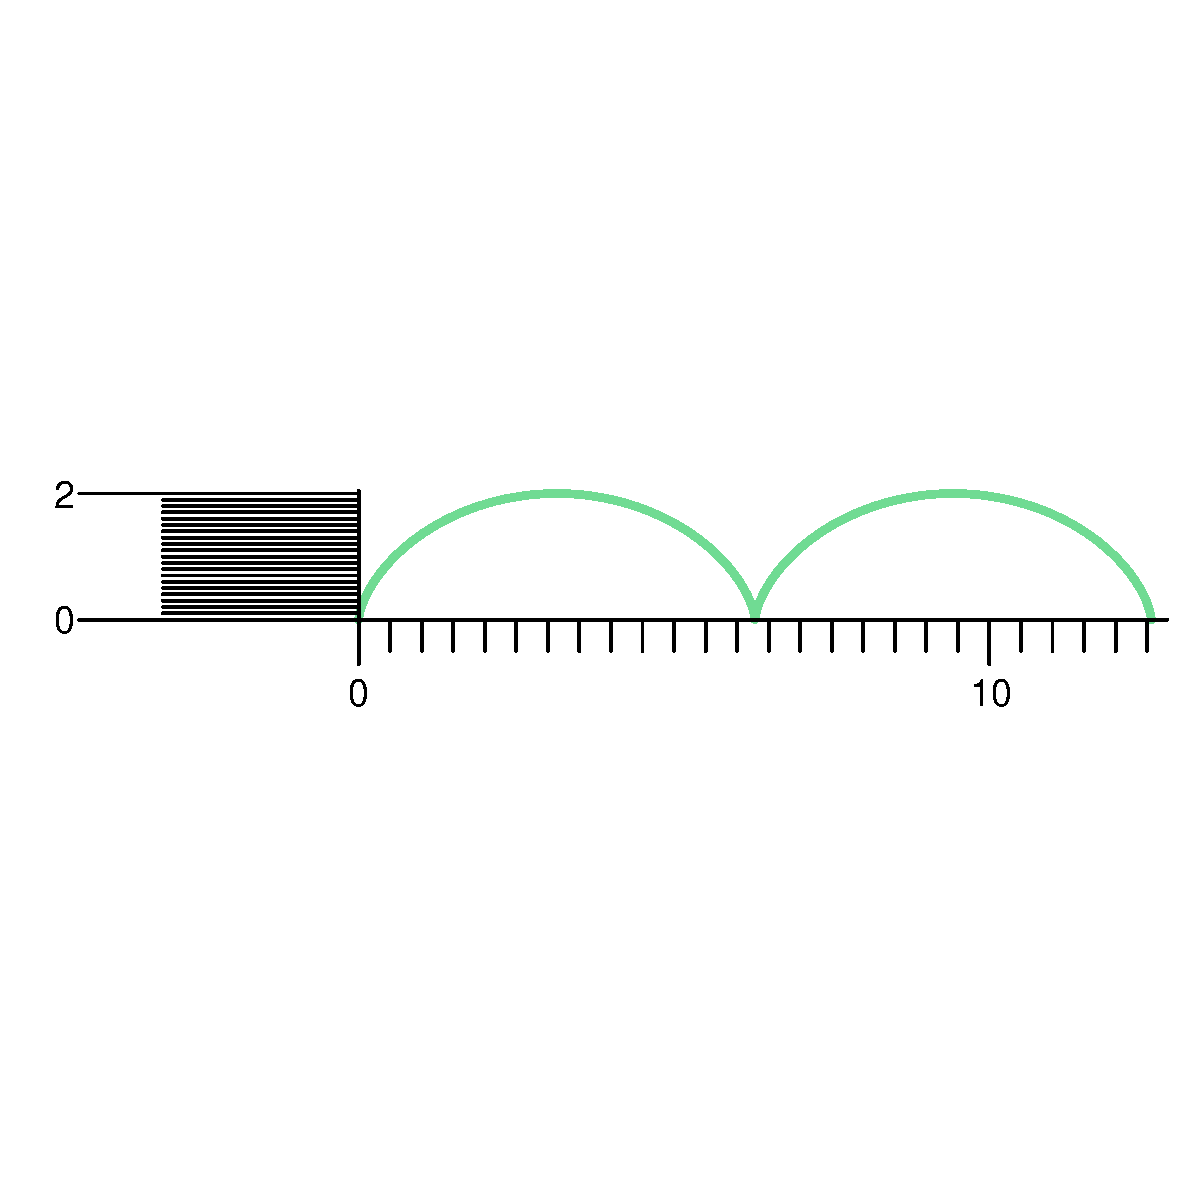
\includegraphics[width=6cm]{cycloide.eps}\\
    \end{center}

        \begin{center}
        Evangelista Torricelli\\
    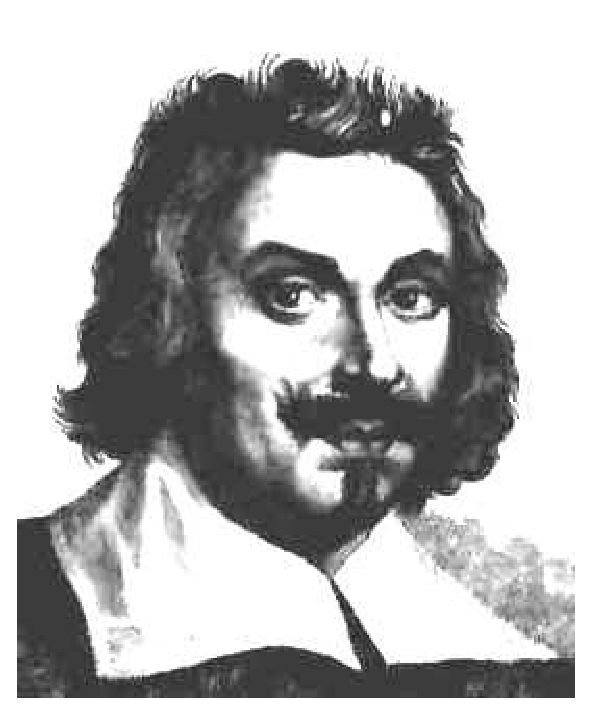
\includegraphics[width=6cm]{tortor.eps}\\
        {\footnotesize http ://www.whyy.org/tv12/franklinfacts/MAR1400.jpg}
    \end{center}

1034-- In which country was John Wallis (1616-1703) born?

a$)$ England \\
b$)$ Belgium \\
c$)$ Greece  \\
d$)$ Iceland \\

Answer : a$)$\\

Feedback :\\
John Wallis was born in England. It is to Wallis that
we owe the symbol $\infty$ for the infinity.
The answer is a$)$.\\

        \begin{center}
        John Wallis\\[2mm]
    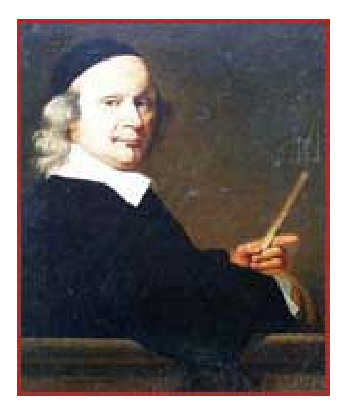
\includegraphics[width=6cm]{walwal.eps}\\
        {\footnotesize http
://curvebank.calstatela.edu/birthdayindex/nov/nov23wallis/john\_wallis2.jpg}
    \end{center}

        \begin{center}
        Angleterre\\
    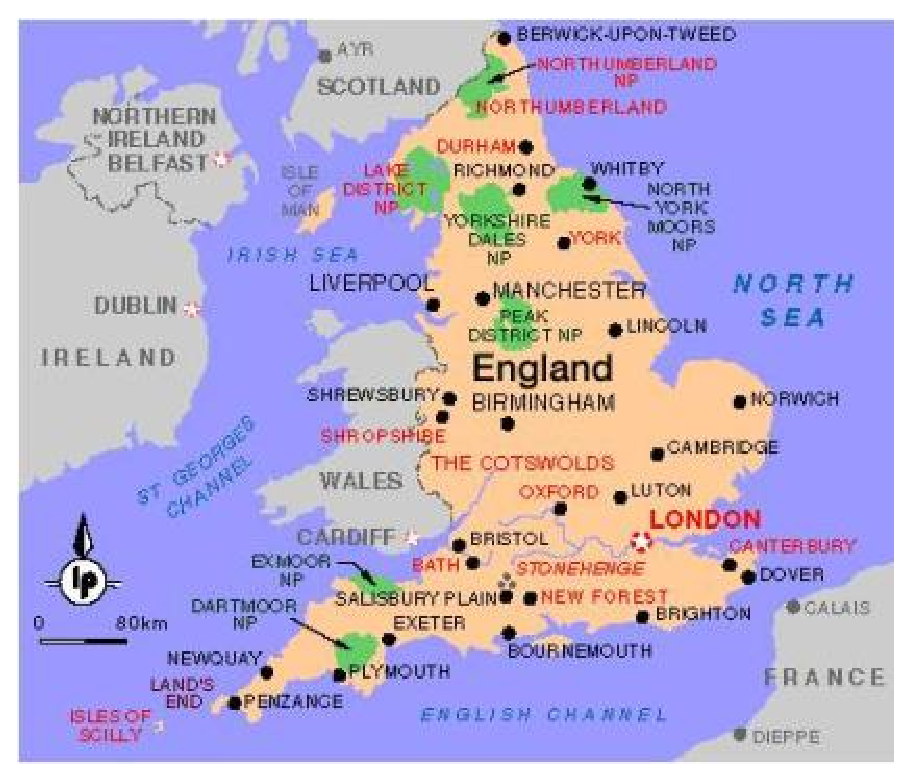
\includegraphics[width=6cm]{ang.eps}\\
        {\footnotesize http
://www.ac-rouen.fr/colleges/hugo-rugles/carte\%20angleterre.jpg}
    \end{center}

1035 * -- Let $p$ be a positive integer. Consider the surface
defined by the function $x^p$ and by the straight lines $x=1$ and
$y=0$. Who was the forst to show that the area of this surface
is $\frac1{p\,+\,1}$ ?

a$)$ Ernest Rutherford \\
b$)$ Euclide d'Alexandrie  \\
c$)$ John Wallis  \\
d$)$ Thal\`es de Milet \\

Answer : c$)$\\

Feedback :\\
John Wallis was the first to find the area of this surface.
The answer is c$)$.\\

        \begin{center}
        John Wallis\\
    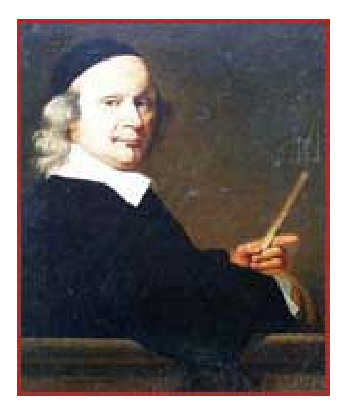
\includegraphics[width=6cm]{walwal.eps}\\
        {\footnotesize http
://curvebank.calstatela.edu/birthdayindex/nov/nov23wallis/john\_wallis2.jpg}
    \end{center}

1036-- Let the sequence
$$\displaystyle{1-\frac1{4(1)^2},\quad\left(1-\frac1{4(1)^2}\right)\left(1-\frac1{4(2)^2}\right),\quad
\left(1-\frac1{4(1)^2}\right)\left(1-\frac1{4(2)^2}\right)\left(1-\frac1{4(3)^2}\right),\quad\ldots}$$
In doing the operations, we get the following sequence :
$$\displaystyle{\frac34,\quad\frac{45}{64},\quad\frac{175}{256},\quad\ldots}$$
John Wallis showed that the terms of this sequence will
stabilize and close up as close as we want to a certain
number. What is that number?

a$)$ $\frac2{\pi}$ \\[2mm]
b$)$ $\frac{\pi}4$  \\[2mm]
c$)$ $\pi$  \\[2mm]
d$)$ $40$\\

Answer : a$)$\\

Feedback :\\
This number is $\frac2{\pi}$. The answer is a$)$. Verify that
the third term gives an approximation of $\frac2{\pi}$. We have
$$\displaystyle{\frac{175}{256}\approx0,6\approx\frac2{\pi}}.$$
\\

1037-- To whom do we owe the symbol $\infty$ to designate the infinity?

a$)$ Al Khwarizmi \\
b$)$ Johannes Diderik Van der Waals   \\
c$)$ John Wallis  \\
d$)$ L\'eonard de Pise \\

Answer : c$)$\\

Feedback :\\
We owe this symbol to John Wallis.
The answer is c$)$.\\

        \begin{center}
        John Wallis\\
    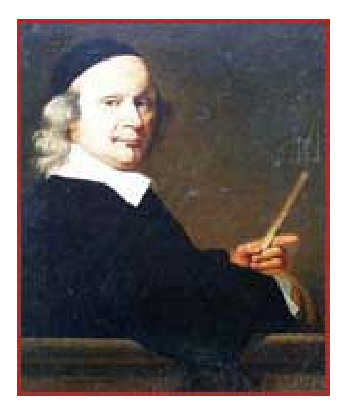
\includegraphics[width=6cm]{walwal.eps}\\
        {\footnotesize http
://curvebank.calstatela.edu/birthdayindex/nov/nov23wallis/john\_wallis2.jpg}
    \end{center}

1038 * -- In what year did John Wallis foresee the
geometrical representation of complex numbers and
showed that the logarithmic function is the opposite of the
exponential function?

a$)$ 1002 \\
b$)$ 1673  \\
c$)$ 1904  \\
d$)$ 2001 \\

Answer : b$)$\\

Feedback :\\
It is in 1673.
The answer is b$)$.\\

        \begin{center}
        John Wallis\\
    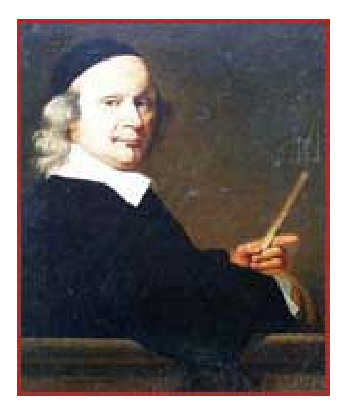
\includegraphics[width=6cm]{walwal.eps}\\
        {\footnotesize http
://curvebank.calstatela.edu/birthdayindex/nov/nov23wallis/john\_wallis2.jpg}
    \end{center}

1039-- Who introduced the systematic use of negative 
and fractional exponents?

a$)$ Galileo Galil\'ee \\
b$)$ Hans Jonas  \\
c$)$ John Wallis  \\
d$)$ Raphael Bombelli \\

Answer : c$)$\\

Feedback :\\
It is John Wallis.
The answer is c$)$.\\

        \begin{center}
        John Wallis\\
    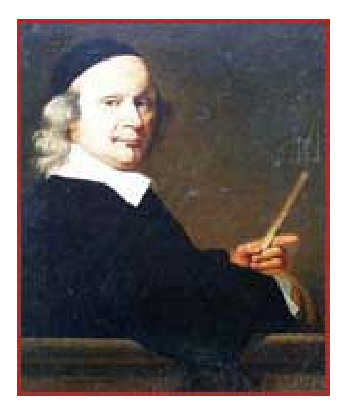
\includegraphics[width=6cm]{walwal.eps}\\
        {\footnotesize http
://curvebank.calstatela.edu/birthdayindex/nov/nov23wallis/john\_wallis2.jpg}
    \end{center}

1040-- In which country was William Brouncker (1620-1684) born?

a$)$ France  \\
b$)$ Greece  \\
c$)$ Ireland \\
d$)$ Jamaica\\

Answer : c$)$\\

Feedback : \\
William Brouncker was born in Ireland.
The answer is c$)$.\\
        \begin{center}
        Ireland\\
    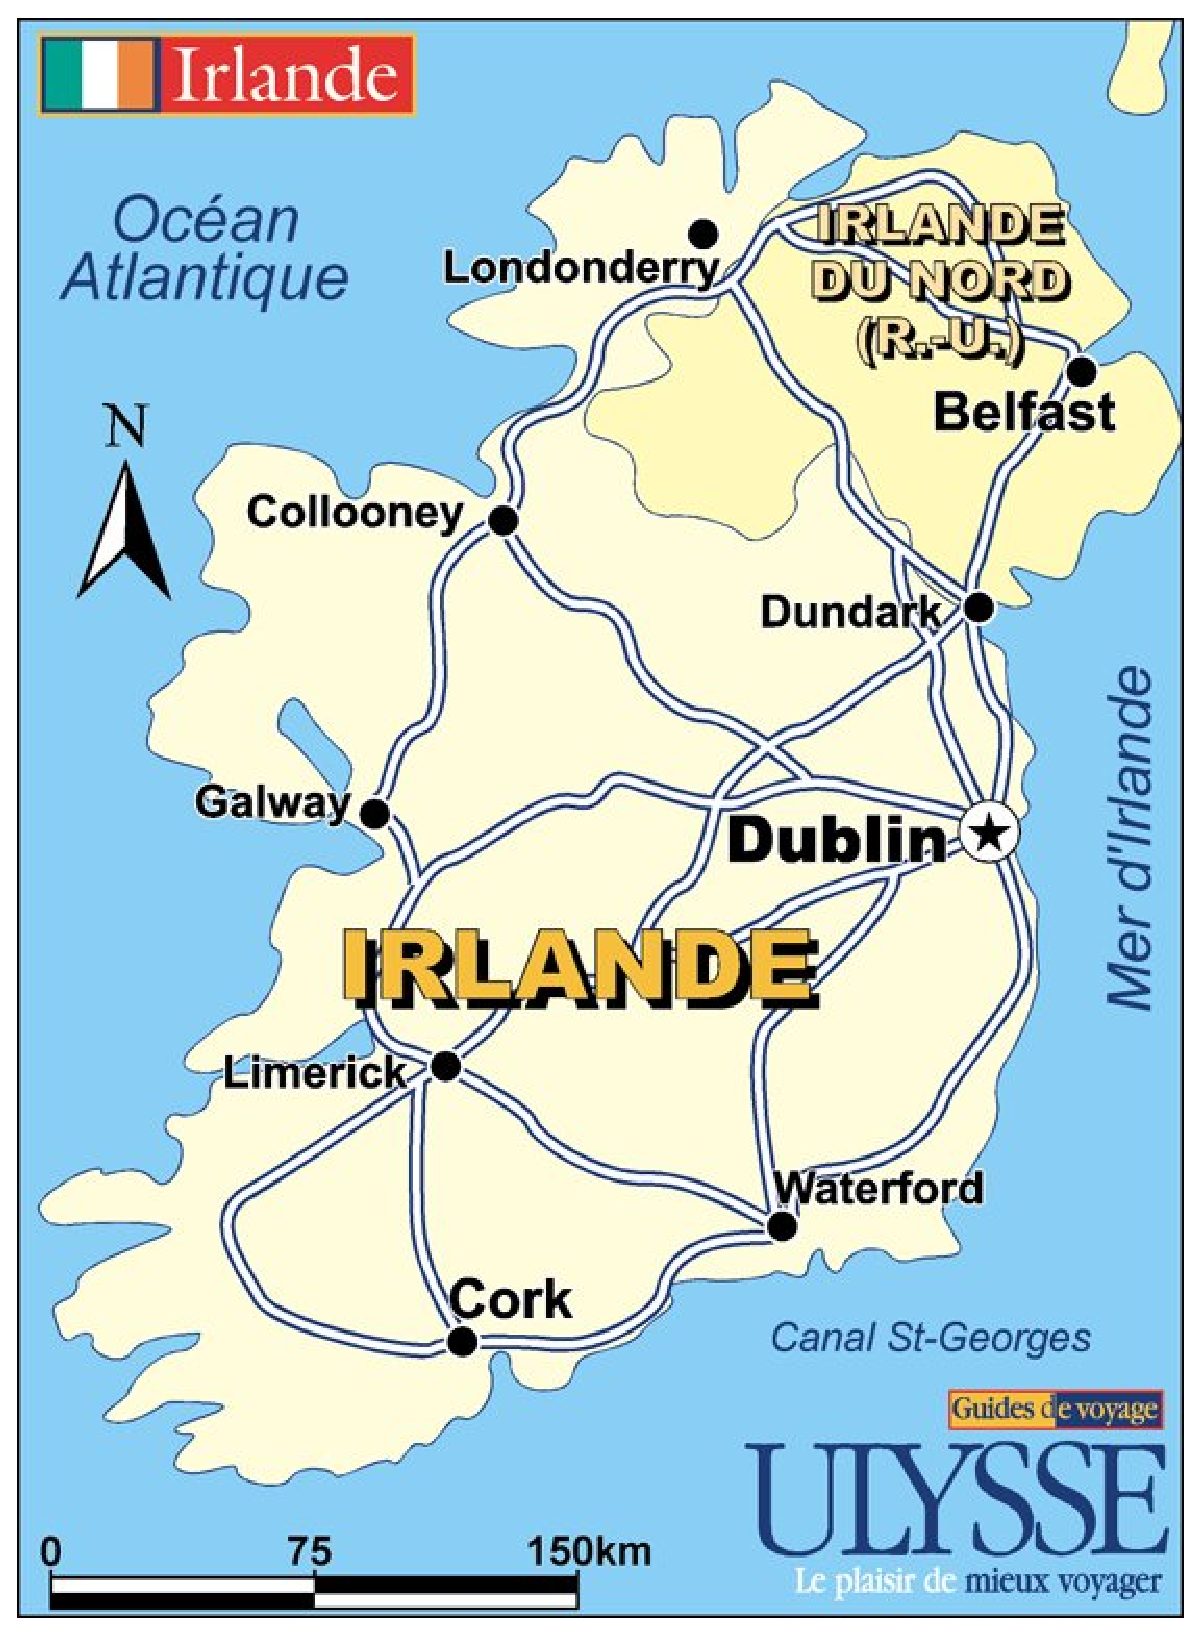
\includegraphics[width=6cm]{irlande.eps}\\
    \end{center}

1041 * -- The equations of type $x^2\,-\,dy^2=1$, where $d>0$
is not a perfect square, are known as {\sl
Pell's equations}. During the years 1657 and 1658, who attained a
method to find the solutions of integers $x$ and $y$ of {\sl
Pell's equations}?

a$)$ Charmid\`es \\
b$)$ John Pell \\
c$)$ Leonhard Euler  \\
d$)$ William Brouncker\\

Answer : d$)$\\

Feedback : \\
William Brouncker attained this method. These equations
are called {\sl Pell's equations} because Euler believed that
it was Pell that found the problem-solving method.
The answer is d$)$.\\

        \begin{center}
        Leonhard Euler\\
    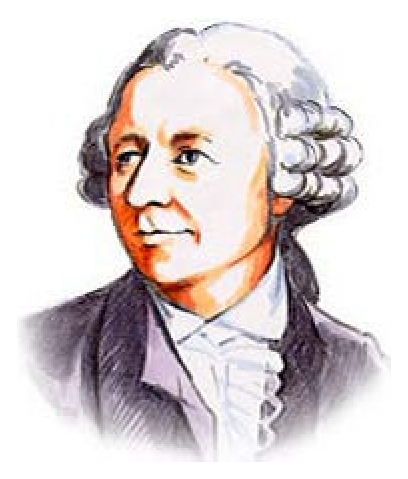
\includegraphics[width=6cm]{euler.eps}\\
        {\footnotesize http
://www.uni-flensburg.de/mathe/zero/mgalerie/euler/euler.jpg}
    \end{center}

1042-- Why do the equations of type $x^2\,-\,dy^2=1$, where
$d>0$ is not a perfect square, are known as
{\sl Pell's equations} even though it was William Brouncker who
attained the solving method?

a$)$ Because Brouncker was Pell's servant. \\
b$)$ Because Euler believed that it was Pell who found the
the problem-solving process.  \\
c$)$ Because Pell had bought the results from Brouncker.  \\
d$)$ Because Pell was the first to study them.\\

Answer : b$)$\\

Feedback : \\
The reason is that Euler believed that it was Pell who had
found their solving process.
The answer is b$)$.\\
        \begin{center}
        Leonhard Euler\\
    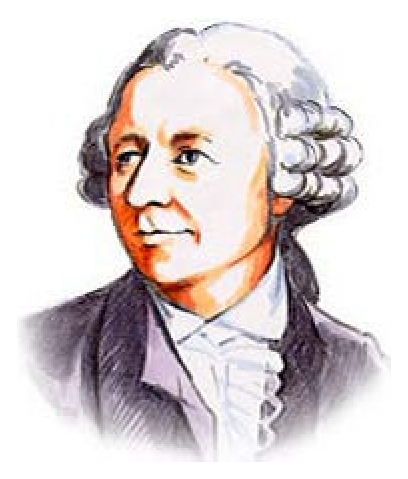
\includegraphics[width=6cm]{euler.eps}\\
        {\footnotesize http
://www.uni-flensburg.de/mathe/zero/mgalerie/euler/euler.jpg}
    \end{center}

1043-- To whom do we owe the formula
$$\displaystyle{\frac{\pi}4=\frac1{1\,+\,\frac{1^2}{2\,+\,\frac{3^2}{2\,+\,\frac{5^2}{2\,+\,\ldots}}}}}\quad?$$

a$)$ Bonaventura Cavalieri \\
b$)$ Epicure \\
c$)$ G\'erard Desargues  \\
d$)$ William Brouncker\\

Answer : d$)$\\

Feedback : \\
We owe this formula to William Brouncker.
The answer is d$)$.\\

1044-- In which country did Nicolaus Mercator (1620-1687) die?

a$)$ Germany \\
b$)$ France  \\
c$)$ Greece  \\
d$)$ Martinique \\

Answer : b$)$\\

Feedback : \\
Mercator died in France.
The answer is b$)$.\\

        \begin{center}
        France\\
    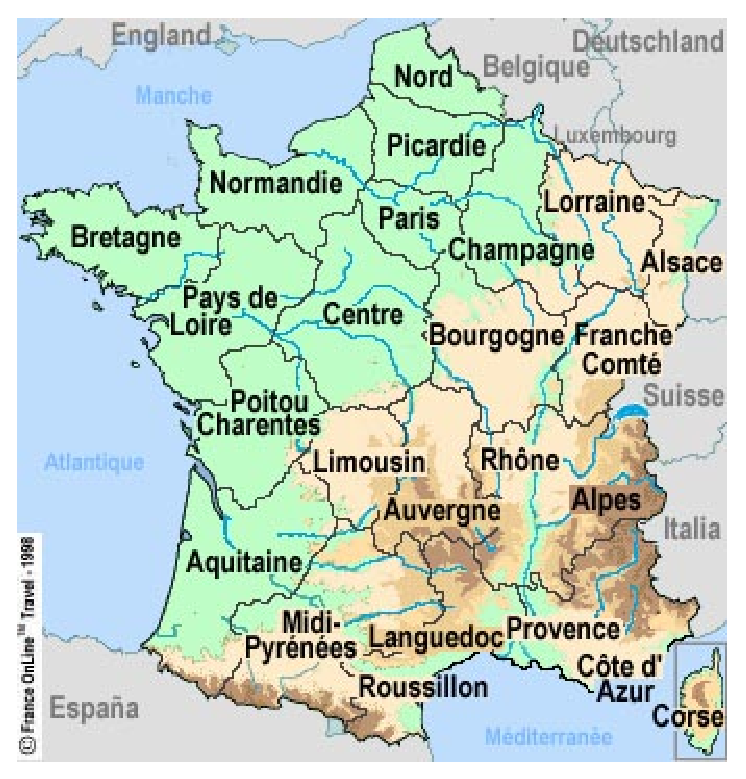
\includegraphics[width=6cm]{france.eps}\\
    \end{center}

1045-- Let the sequence of functions
$$\displaystyle{x,\quad x-\frac{x^2}2,\quad
x-\frac{x^2}2\,+\,\frac{x^3}3,\quad
x-\frac{x^2}2\,+\,\frac{x^3}3-\frac{x^4}4,\quad
x-\frac{x^2}2\,+\,\frac{x^3}3-\frac{x^4}4\,+\,\frac{x^5}5,\quad\ldots}$$
John Wallis showed that the terms of this sequence will
stabilize and close up as close as wanted to a
certain function. What is this function?

a$)$ $\ln(1\,-\,x)$ \\
b$)$ $\ln(1\,+\,yx)$  \\
c$)$ $\sin x$  \\
d$)$ $x\,+\,1$

Answer : b$)$\\

Feedback : \\
This function $\ln(1\,+\,x)$. The answer is b$)$.
For exmmple, verify that for $x=0,5$ the fifth term of the
sequence gives an approximation of $\ln(1\,+\,0,5)=\ln(1,5)$. We have
$$0,5-\frac{0,5^2}2\,+\,\frac{0,5^3}3-\frac{0,5^4}4\,+\,\frac{0,5^5}5\approx0,41\approx\ln(1,5).$$
\\

1046-- What was Blaise Pascal's first work?

a$)$ {\sl Essay on Conics} \\
b$)$ {\sl Le Malade imaginaire}  \\
c$)$ {\sl Opticks}  \\
d$)$ {\sl Philosophiae naturalis principia mathematica}\\

Answer : a$)$\\

Feedback : \\
Pascal's first work is {\sl Essay on
Conics} which he published in 1640. The answer is a$)$.

        \begin{center}
        Blaise Pascal\\
    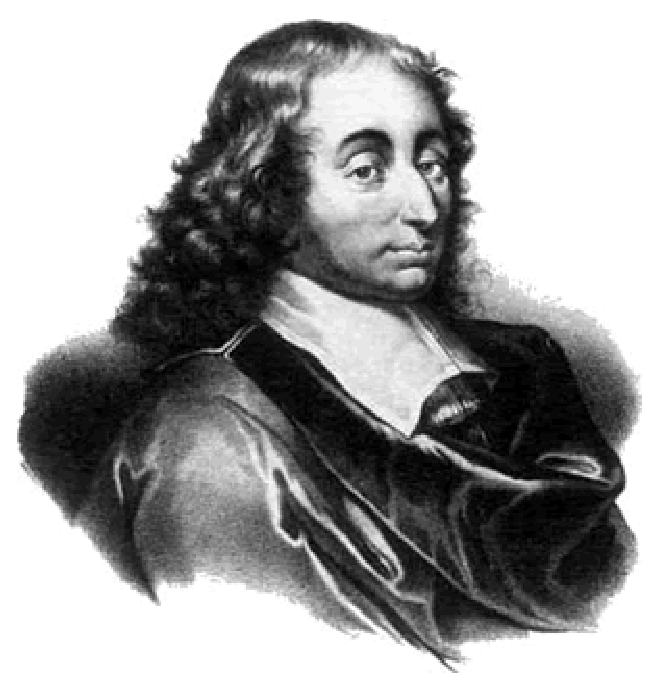
\includegraphics[width=6cm]{pascal.eps}\\
        {\footnotesize http
://www.thocp.net/biographies/pictures/pascal\_blaise2.gif}
    \end{center}

1047-- For what reason did Blaise Pascal invent
a machine to calculate?

a$)$ To help the accountants of the King of England evaluate the endowment
of the country.   \\
b$)$ To help is father in his work as a tax collector for
Upper Normandy.  \\
c$)$ To calculate the population of France's big cities. \\
d$)$ To facilitate his own mathematical calculations.

Answer : b$)$\\

Feedback : \\
Blaise Pascal wanted to help his father in his work as
a tax collector for Upper Normandy.
The answer is b$)$.\\

        \begin{center}
        Blaise Pascal\\
    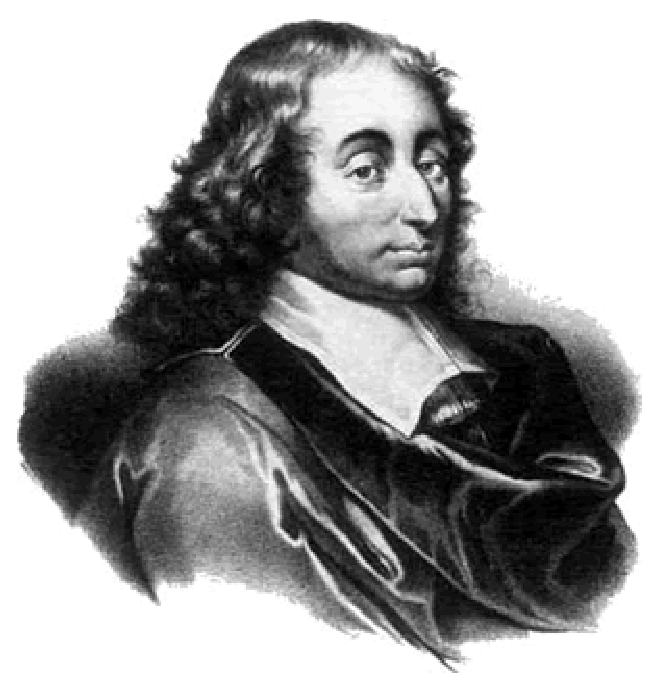
\includegraphics[width=6cm]{pascal.eps}\\
        {\footnotesize http
://www.thocp.net/biographies/pictures/pascal\_blaise2.gif}
    \end{center}

1048-- Mathematicians have often done well in the other
sciences. Who observed, in 1648, that the atmospheric pressure
decreases with altitude?

a$)$ Blaise Pascal \\
b$)$ Christopher Wren   \\
c$)$ Gottfried Wilhelm Leibniz  \\
d$)$ Jean-Pierre Serre \\

Answer : a$)$\\

Feedback : \\
Blaise Pascal made this observation.
The answer is a$)$.\\

        \begin{center}
        Blaise Pascal\\
    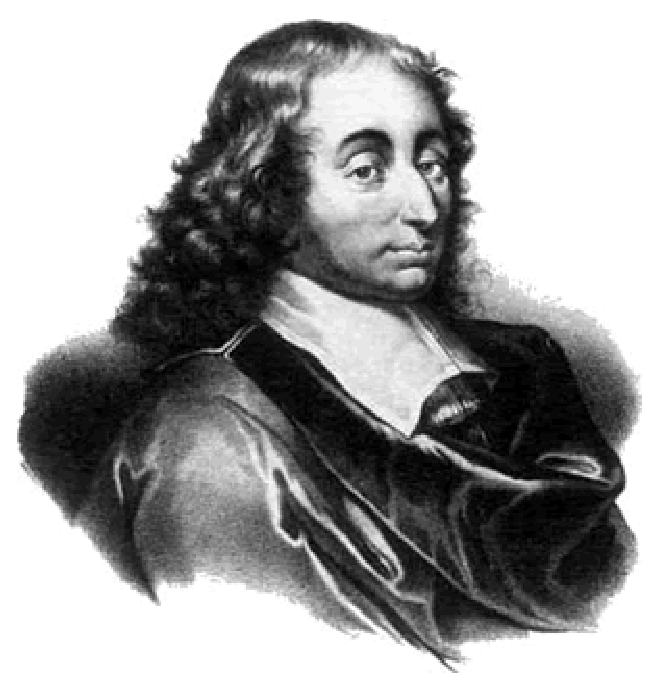
\includegraphics[width=6cm]{pascal.eps}\\
        {\footnotesize http
://www.thocp.net/biographies/pictures/pascal\_blaise2.gif}
    \end{center}

1049-- Which work did Blaise Pascal publish in 1654?

a$)$ {\sl Discourse on the Origin and Basis of Inequality Among Men} \\
b$)$ {\sl Opticks}  \\
c$)$ {\sl Philosophiae naturalis principia mathematica}  \\
d$)$ {\sl Treatise on the Arithmetic of Triangles}\\

Answer : d$)$\\

Feedback : \\
Pascal published the work {\sl Treatise on the Arithmetic 
of Triangles}.
The answer is d$)$.\\

        \begin{center}
        Blaise Pascal\\
    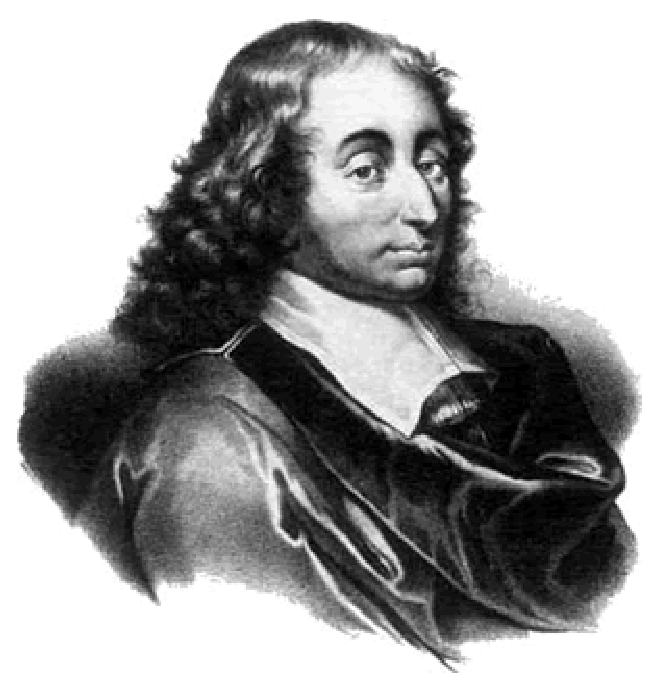
\includegraphics[width=6cm]{pascal.eps}\\
        {\footnotesize http
://www.thocp.net/biographies/pictures/pascal\_blaise2.gif}
    \end{center}

1050-- Who came up with the foundations of the probability theory in
1654?

a$)$ Blaise Pascal \\
b$)$ Jakob Bernoulli  \\
c$)$ Jean-Jacques Rousseau \\
d$)$ John Machin\\

Answer : a$)$\\

Feedback : \\
It is Blaise Pascal.
The answer is a$)$.\\

        \begin{center}
        Blaise Pascal\\
    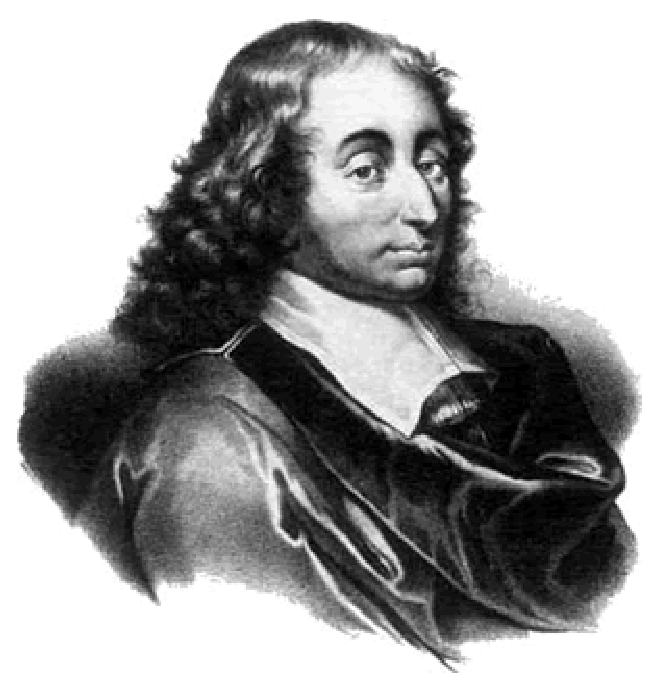
\includegraphics[width=6cm]{pascal.eps}\\
        {\footnotesize http
://www.thocp.net/biographies/pictures/pascal\_blaise2.gif}
    \end{center}

1051-- The curve defined by the path of a point on the edge of 
circular wheel as the wheel rolls along a straight line is called a 
cycloid. In what year did Blaise Pascal calculate the volume and 
the area of the shape created by making a cycloid arc turn around 
the $x$-axis?

a$)$ 26 \\
b$)$ 765  \\
c$)$ 1658  \\
d$)$ 1927\\

Answer : c$)$\\

Feedback : \\
Pascal made these calculations in 1658.
The answer is c$)$.\\

        \begin{center}

Cyclo\"ide\\
    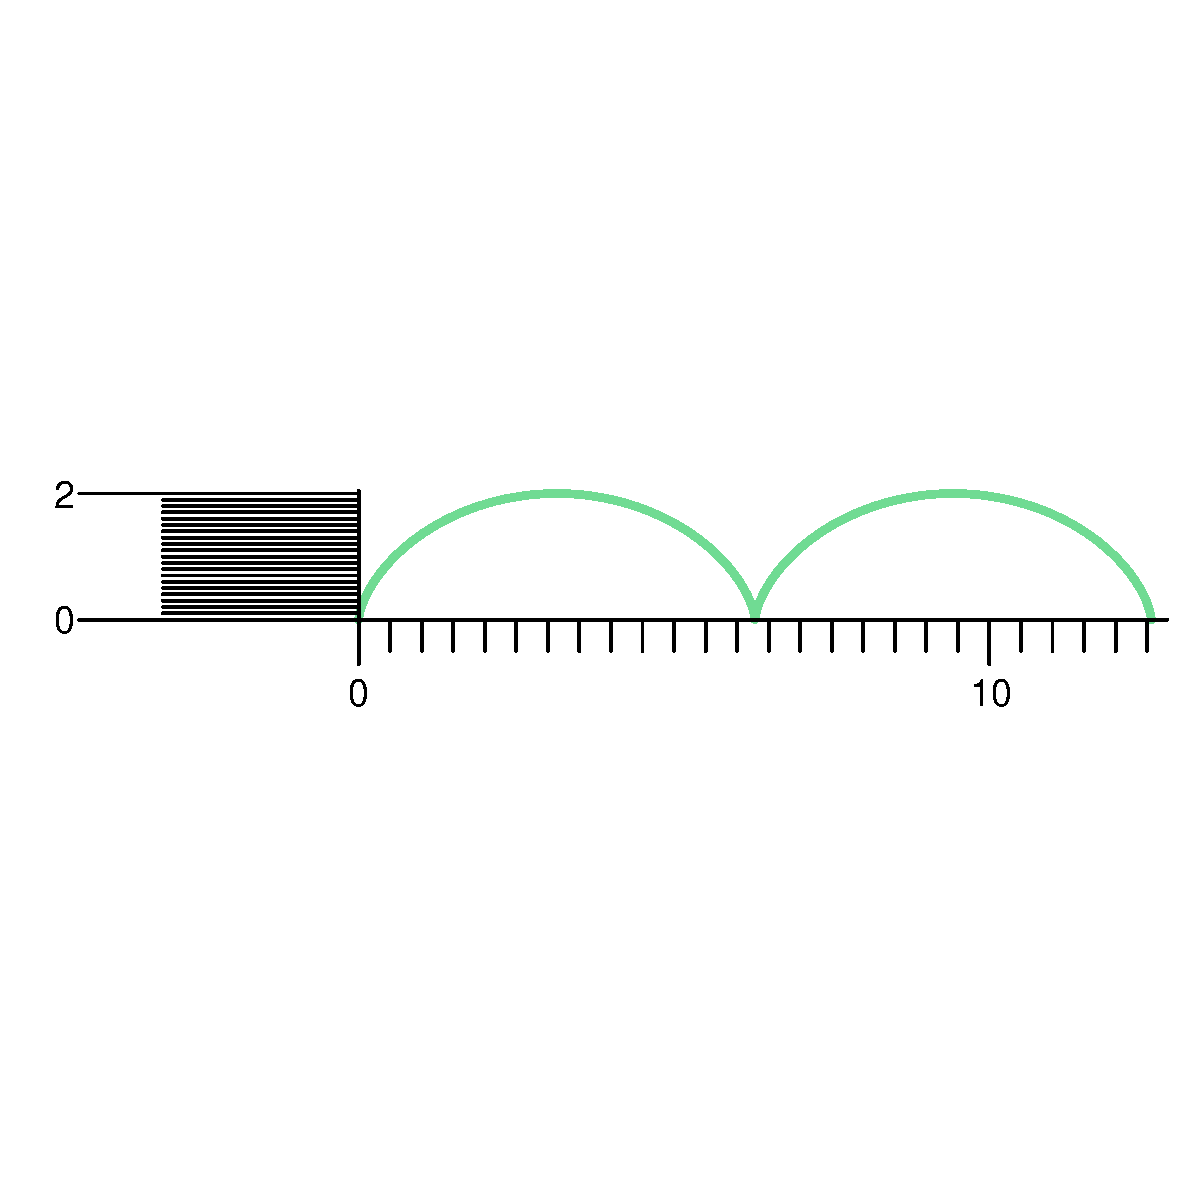
\includegraphics[width=6cm]{cycloide.eps}\\
    \end{center}

        \begin{center}
        Blaise Pascal\\
    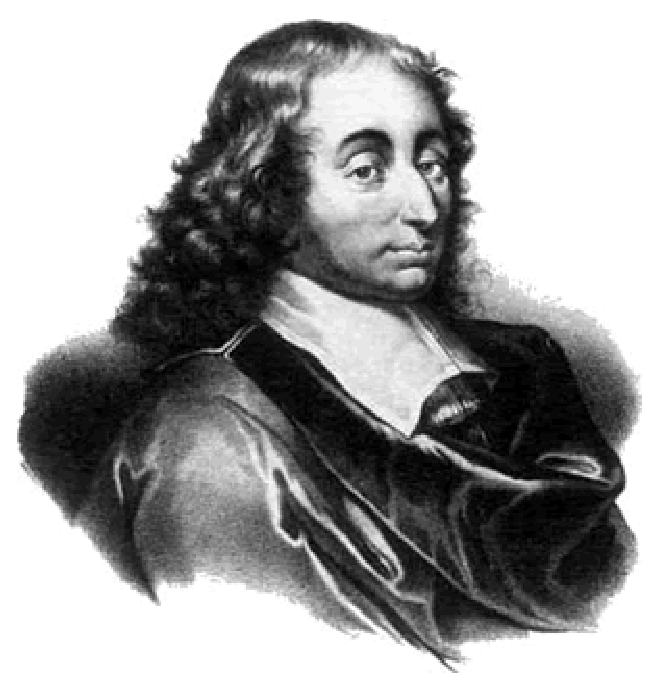
\includegraphics[width=6cm]{pascal.eps}\\
        {\footnotesize http
://www.thocp.net/biographies/pictures/pascal\_blaise2.gif}
    \end{center}

1052-- To which activity did Blaise Pascal decide to
devote his life?

a$)$ Agriculture \\
b$)$ Painting  \\
c$)$ Religious reflection\\
d$)$ Golf\\

Answer : c$)$\\

Feedback : \\
Pascal decided to devote his life to religious reflection.
The answer is c$)$.\\

        \begin{center}
        Blaise Pascal\\
    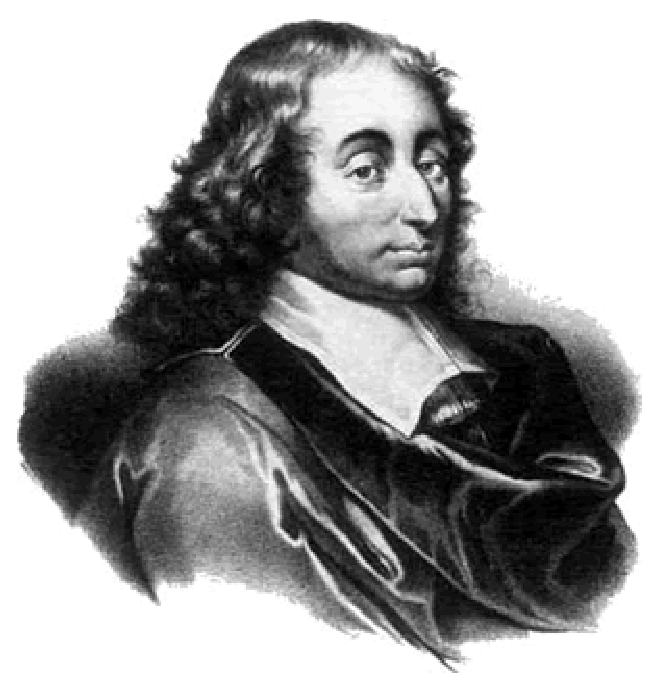
\includegraphics[width=6cm]{pascal.eps}\\
        {\footnotesize http
://www.thocp.net/biographies/pictures/pascal\_blaise2.gif}
    \end{center}

1053-- What brought Blaise Pascal, at a particularly
difficult period of his life, to reunite with
mathematics?

a$)$ He was in jail and had nothing better to do. \\
b$)$ A chronic toothache  \\
c$)$ A heartbreak\\
d$)$ His father obliged him to do mathematics.\\

Answer : b$)$\\

Feedback : \\
It was a chronic toothache that restrained Pascal from sleeping. He
then found some comfort in doing mathematics,
which brought him to discover great things.
The answer is b$)$.\\

        \begin{center}
        Blaise Pascal\\
    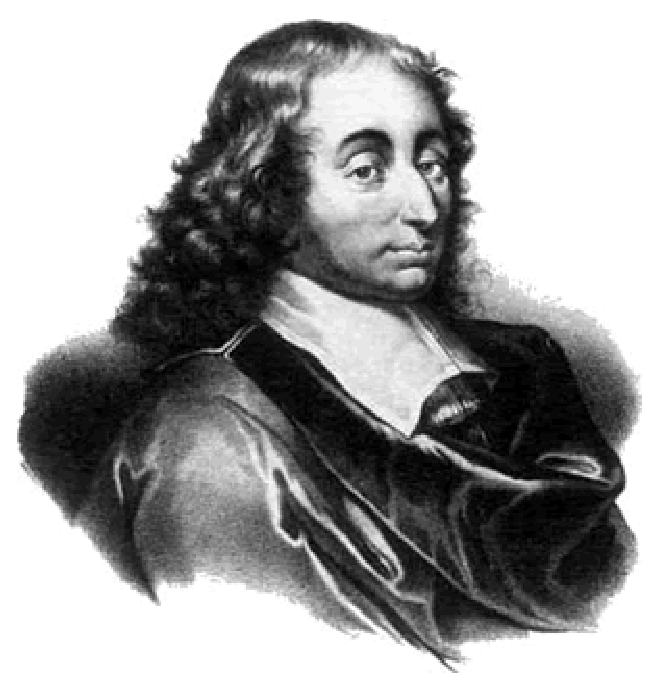
\includegraphics[width=6cm]{pascal.eps}\\
        {\footnotesize http
://www.thocp.net/biographies/pictures/pascal\_blaise2.gif}
    \end{center}

1054-- Which mathematician was at the origins of public transit?

a$)$ Blaise Pascal \\
b$)$ Charles Darwin  \\
c$)$ Leonhard Euler  \\
d$)$ Maria Gaetana Agnesi\\

Answer : a$)$\\

Feedback : \\
Blaise Pascal was at the origins of public transit. He wanted
to help the less fortunate.
The answer is a$)$.\\

        \begin{center}
        Blaise Pascal\\
    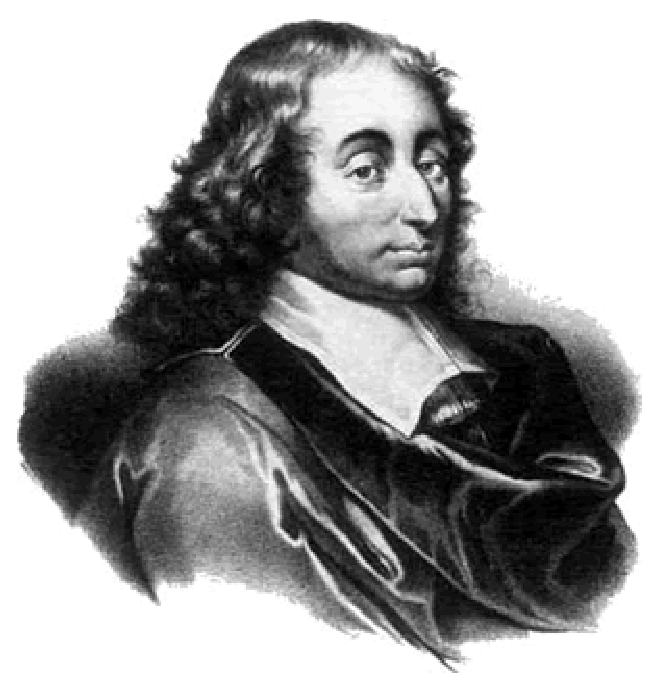
\includegraphics[width=6cm]{pascal.eps}\\
        {\footnotesize http
://www.thocp.net/biographies/pictures/pascal\_blaise2.gif}
    \end{center}

1055-- For which reason did Blaise Pascal want to introduce a
public transit system?

a$)$ Because he did not like driving \\
b$)$ To reduce pollution \\
c$)$ To reduce traffic jams \\
d$)$ To help the less fortunate people \\

Answer : d$)$\\

Feedback : \\
Pascal wanted to help the less fortunate.
The answer is d$)$.\\

        \begin{center}
        Blaise Pascal\\
    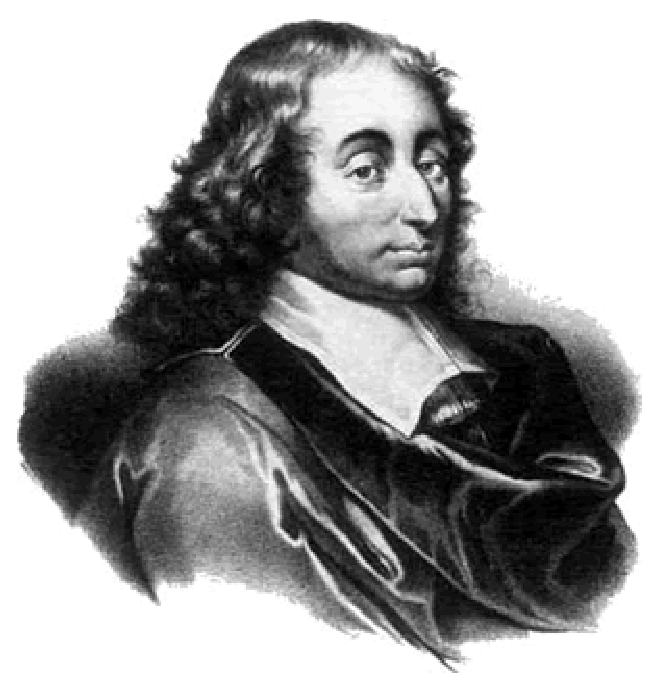
\includegraphics[width=6cm]{pascal.eps}\\
        {\footnotesize http
://www.thocp.net/biographies/pictures/pascal\_blaise2.gif}
    \end{center}

1056-- In which country was Christian Huygens (1629-1695) born?

a$)$ France \\
b$)$ Greece  \\
c$)$ Mauritius  \\
d$)$ Netherlands \\

Answer : d$)$\\

Feedback : \\
Christian Huygens was born in the Netherlands. Huygens published the
first work on the calculation of probabilities.
The answer is d$)$.\\

        \begin{center}
        Christian Huygens\\
    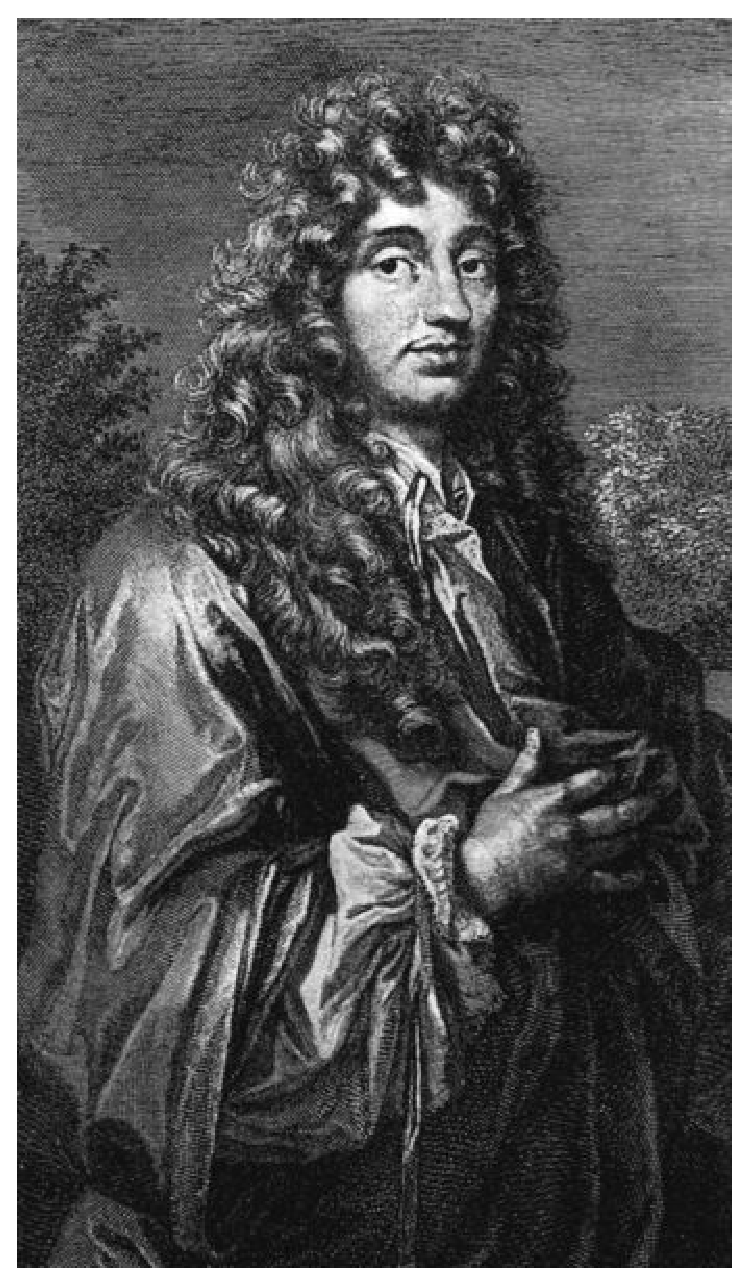
\includegraphics[width=6cm]{huygens.eps}\\
        {\footnotesize http
://www.th.physik.uni-frankfurt.de/$\sim$jr/gif/phys/huygens.jpg}
    \end{center}

        \begin{center}
        Netherlands\\
    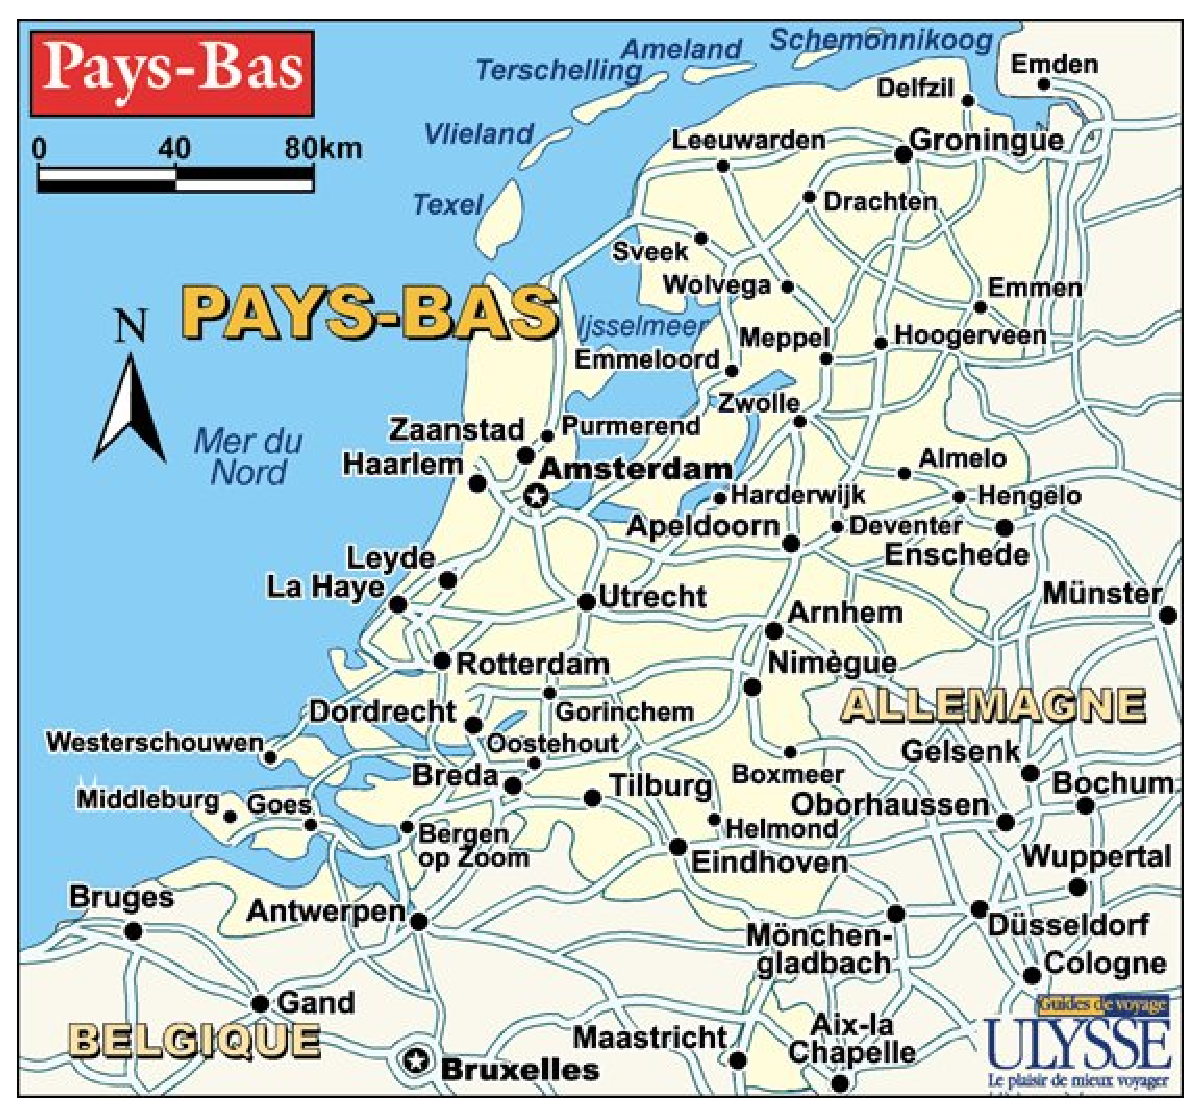
\includegraphics[width=6cm]{pays.eps}\\
    \end{center}

1057-- Who published the first work on the calculation of
probabilities?

a$)$ Carl Friedrich Gauss \\
b$)$ Christian Huygens \\
c$)$ Gaspard Monge  \\
d$)$ Voltaire  \\

Answer : b$)$\\

Feedback : \\
It is Christian Huygens.
The answer is b$)$.\\

        \begin{center}
        Christian Huygens\\
    \includegraphics[width=6cm]{huygens.eps}\\
        {\footnotesize http
://www.th.physik.uni-frankfurt.de/$\sim$jr/gif/phys/huygens.jpg}
    \end{center}

1058-- Mathematicians have many purposes in 
their everyday life. Which mathematician originated the first
pendulum clock  in 1656?

a$)$ Augustin Louis Cauchy \\
b$)$ Christian Huygens  \\
c$)$ John Forbes Nash  \\
d$)$ Niels Henrik Abel \\

Answer : b$)$\\

Feedback : \\
The first pendulum clock was created by Christian
Huygens.
The answer is b$)$.\\

        \begin{center}
        Christian Huygens\\
    \includegraphics[width=6cm]{huygens.eps}\\
        {\footnotesize http
://www.th.physik.uni-frankfurt.de/$\sim$jr/gif/phys/huygens.jpg}
    \end{center}

1059-- In 1655, mathematician Christian Huygens discovered a
moon. Around which planet does this moon gravitate?

a$)$ Mercury \\
b$)$ Pluton  \\
c$)$ Saturn  \\
d$)$ Uranus \\

Answer : c$)$\\

Feedback : \\
This moon gravitates around Saturn. The next year, Huygens
discovered the true shape of the rings of Saturn.
The answer is c$)$.\\

        \begin{center}
        Christian Huygens\\
    \includegraphics[width=6cm]{huygens.eps}\\
        {\footnotesize http
://www.th.physik.uni-frankfurt.de/$\sim$jr/gif/phys/huygens.jpg}
    \end{center}


1060 * -- The curve defined by the path of a point on the edge of circular 
wheel as the wheel rolls along a straight line is called a cycloid. Consider
the reflection of a cycloid arc with reference to the straight line
that creates it. This curve is called an inverted cycloid.
Christian Huygens demonstrated that if we were to place a marble anywhere
on an inverted cycloid, with the exception of its center,
the time it would take for the marble to come back to its starting point
is independent of where it is placed. How do we call this property?

a$)$ The movement property  \\
b$)$ The sliding property  \\
c$)$ The material object property  \\
d$)$ The tautochrone property \\

Answer : d$)$

Feedback : \\
It is the tautochrone property.
The answer is d$)$.\\

        \begin{center}

Cycloid        \\
    \includegraphics[width=6cm]{cycloide.eps}\\
    \end{center}

1061-- Amongst the following, which mathematician was born in England?

a$)$ Abu Ali al-Haitham (965-1039) \\
b$)$ Christopher Wren (1632-1723) \\
c$)$ L\'eonard de Pise (1170-1250) \\
d$)$ Thal\`es de Milet (624-547 av. J.-C.)

Answer : b$)$\\

Feedback : \\
Christopher Wren was born in England. Wren was a
mathematician but he was also the architect of the
St-Paul's Cathedral, in London.
The answer is b$)$.\\

        \begin{center}
        Christopher Wren\\
    \includegraphics[width=6cm]{wren2.eps}\\
        {\footnotesize http ://intranet.arc.miami.edu/rjohn/Spring2000/New\\
        \%20slides/Jones\%20and\%20Wren\%20slides/Christopher\%20Wren.jpg}
    \end{center}

        \begin{center}
        St-Paul's Cathedral, London\\
    \includegraphics[width=6cm]{stpaul.eps}\\
        {\footnotesize http
://3demi.net/photos/voyages/europe/londres/images/04-03-12\_19h17m08s.jpg}
    \end{center}

1062 * -- The curve defined by the path of a point on the edge of circular 
wheel as the wheel rolls along a straight line is called a cycloid. Who
demonstrated that the lenght of the arc of a cycloid was of 4 times
the diameter of the circle that creates it?

a$)$ Christopher Wren\\
b$)$ \'Evariste Galois \\
c$)$ Honor\'e de Balzac \\
d$)$ Pafnuty Lvovich Chebyshev\\

Answer : a$)$\\

Feedback : \\
Christopher Wren demonstrated this fact.
The answer is a$)$.\\

1063-- Mathematician Christopher Wren was also an architect.
What famous cathedral did he design?

a$)$ The Cathedral of Our Lady of Chartres  \\
b$)$ The Cathedral of Our Lady of Amiens \\
c$)$ Cathedral of Notre-Dame, Reims \\
d$)$ St-Paul's Cathedral, London \\

Answer : d$)$\\

Feedback : \\
Wren designed the St-Paul's Cathedral, London.
The answer is d$)$.\\

1064-- From which country was James Gregory (1638-1675) from?

a$)$ Scotland \\
b$)$ France  \\
c$)$ Greece  \\
d$)$ Panama \\

Answer : a$)$ \\

Feedback : \\
James Gregory was from Scotland. This mathematician got
interesting results for functions $\arctan x$,
$\arcsin x$ et $\tan x$.
The answer is a$)$.\\

1065-- Let this sequence of functions
$$\displaystyle{x,\quad x-\frac{x^3}3,\quad
x-\frac{x^3}3\,+\,\frac{x^5}5,\quad
x-\frac{x^3}3\,+\,\frac{x^5}5-\frac{x^7}7,\quad
x-\frac{x^3}3\,+\,\frac{x^5}5-\frac{x^7}7\,+\,\frac{x^9}9,\quad\ldots}$$
James Gregory showed that the terms of this sequence will
stabilize and get closer, as near as we want, to a certain function. 
What is that function?

a$)$ $\arcsin(x)$ \\
b$)$ $\arctan(x)$  \\
c$)$ $\sqrt x$  \\
d$)$ $x\,+\,2$\\

Answer : b$)$\\

Feedback : \\
The function is $\arctan(x)$. The answer is b$)$.\\
Verify, for example that for $x=1$ the 8th term of the sequence
will give an approxiamtion of $\arctan(1)$. We have
$$1-\frac{1^3}3\,+\,\frac{1^5}5-\frac{1^7}7\,+\,\frac{1^9}9-\frac{1^{11}}{11}\,+\,\frac{1^{13}}{13}-\frac{1^{15}}{15}\approx0,8\approx\arctan(1).$$


1066 * -- Just as circles, curves can have
tangents in one point. Who was the first to highlight
the link between the calculation of the area underneath 
a curve and the problem of tangents?

a$)$ Charles Baudelaire \\
b$)$ Charles Hermite \\
c$)$ James Gregory  \\
d$)$ Richard Dedekind \\

Answer : c$)$ \\

Feedback : \\
It is James Gregory.
The answer is c$)$.\\

1067 * -- How do we call the theorem, already known by
Isaac Newton, for which $\int_a^bf(x)dx=F(b)\,-\,F(a)$, where
$F'(x)=f(x)$?

a$)$ The fundamental theorem of algebra \\
b$)$ The fundamental theorem of arithmetics  \\
c$)$ The fundamental theorem of the theory of functions  \\
d$)$ The fundamental theorem of calculus \\

Answer : d$)$ \\

Feedback : \\
It is the fundamental theorem of calculus.
The answer is d$)$.\\

1068-- Mathematician Isaac Newton contributed a lot to
astronomy. In 1671, he made a telescope. What was the
magnification factor of his telescope?

a$)$ 3 times \\
b$)$ 40 times  \\
c$)$ 400 times  \\
d$)$ 1000 times \\

Answer : b$)$ \\

Feedback : \\
The magnification factor was of 40 times.
The answer is b$)$.\\

1069-- Mathematician Isaac Newton contributed a lot to
physics. Amongst the following four, which conclusion was drawn by Newton?

a$)$ Light is constituted of photons. \\
b$)$ Light is made of substance rather than waves.  \\
c$)$ Light is a \og mix of different colors \fg .  \\
d$)$ The speed of light is constant.\\

Answer : c$)$ \\

Feedback : \\
Newton discovered that light is a \og mix of
different colors\fg .
The answer is c$)$.\\

1070-- Which work did Isaac Newton publish in 1687?

a$)$ {\sl Candide} \\
b$)$ {\sl Opticks}  \\
c$)$ {\sl Philosophiae naturalis principia mathematica}  \\
d$)$ {\sl Trait\'e sur le triangle arithm\'etique}\\

Answer : c$)$\\

Feedback : \\
Newton published {\sl Philosophiae naturalis principia mathematica}.
The answer is c$)$.\\

1071-- Mathematician Isaac Newton contributed a lot to
physics. Amongst the following, which one corresponds to the
field of physics for which Isaac Newton is the initiator ?

a$)$ {\sl Astronomy} \\
b$)$ {\sl Fluid mechanics}  \\
c$)$ {\sl Quantum mechanics}  \\
d$)$ {\sl theory of magnetism}\\

Answer : b$)$\\

Feedback : \\
Newton is the foundeur of the {\sl fluid mechanics}.
The answer is b$)$.\\

1072 * -- Let the sequence of functions
$$\displaystyle{1\,+\,rx,\quad 1\,+\,rx\,+\,\frac{r(r\,-\,1)}{2!}x^2,\quad
1\,+\,rx\,+\,\frac{r(r\,-\,1)}{2!}x^2\,+\,\frac{r(r\,-\,1)(r\,-\,2)}{3!}x^3,\quad
\ldots}$$
where $n!\,=1\times2\times3\times\ldots\times n$. What is 
the name of the theorem that states that the terms of this sequence
will stabilize and close up as close as wanted to
function $(1\,+\,x)^r$ ?

a$)$ {\sl B\'ezout's theorem} \\
b$)$ {\sl Strange function theorem}  \\
c$)$ {\sl Generalized binomial theorem}  \\
d$)$ {\sl Fundamental theorem of algebra}\\

Answer : c$)$\\

Feedback : \\
It is the {\sl Generalized binomial theorem}. For example, 
for $r=1$ and $x=2$, all the terms of the sequence have a value of
$1\,+\,1(2)\,+\,0=3$ and the function also has a value of
$(1\,+\,2)^1=1\,+\,2=3$.
The answer is c$)$.\\

1073 * -- Which mathematician obtained in 1666 the following formula:
$$\displaystyle{\pi=\frac{3\sqrt3}4\,+\,24\left(\frac1{12}-\frac1{5\cdot2^5}-\frac1{28\cdot2^7}-\frac1{72\cdot2^9}-\ldots\right)}\quad?$$

a$)$ Ferdinand Lindemann \\
b$)$ Isaac Newton  \\
c$)$ John Charles Fields  \\
d$)$ Pythagore\\

Answer : b$)$\\

Feedback : \\
Isaac Newton achieved this formula.
The answer is b$)$.\\

1074-- Who adapted {\sl Newton's method} thus allowing one to find
the roots of certain functions?

a$)$ Bertrand Russell \\
b$)$ Emmy Noether  \\
c$)$ Joseph Raphson  \\
d$)$ Le roi George IV\\

Answer : c$)$\\

Feedback : \\
Joseph Raphson adapted this method.
The answer is c$)$.\\

1075-- In which work did Newton mention God's Omnipresence?

a$)$ {\sl Ars magna} \\
b$)$ {\sl Opticks}  \\
c$)$ {\sl La Peau de chagrin}  \\
d$)$ {\sl Principia}\\

Answer : b$)$\\

Feedback : \\
Newton mentionned God's Omnipresence in his work called
{\sl Opticks}.
The answer is b$)$.\\

1076-- It is said that Newton was constantly carrying a small notebook 
with him. What was he writing down in this notebook?

a$)$ mathematical formulas \\
b$)$ The names of new people he would meet.  \\
c$)$ His sins \\
d$)$ The position of the stars at night\\

Answer : c$)$\\

Feedback : \\
Newton wrote down his sins in it.
The answer is c$)$.\\

1077-- Which of the following mathematicians was from
Leipzig, nowadays a city of Germany?

a$)$ Gottfried Wilhelm Leibniz (1646-1716) \\
b$)$ Hippocrate de Chios (470-410 av. J.-C.) \\
c$)$ Ivan Matveevtich Vinogradov (1891-1983) \\
d$)$ J\'anos von Neumann (1903-1957) \\

Answer : a$)$\\

Feedback : \\
Gottfried Wilhelm Leibniz was from Leipzig. He is known
for his work on differential and integral calculus, a
notion now intergrated in the collegiate school program.
The answer is a$)$.\\

1078 * -- Who was the first to use the notation $\int f(x)dx$ ?

a$)$ Abraham Robinson \\
b$)$ Gottfried Wilhelm Leibniz \\
c$)$ Nicolas Bourbaki \\
d$)$ Victor Hugo\\

Answer : b$)$\\

Feedback : \\
Gottfried Wilhelm Leibniz was the first one to use this
notation.
The answer is b$)$.\\

1079 * -- Who attained, in 1675, the formula for the derivative of the 
product of the functions : $(fg)'=f'g\,\,+\,\,fg'$ ?

a$)$ Archim\`ede de Syracuse \\
b$)$ Gottfried Wilhelm Leibniz \\
c$)$ Guy de Maupassant \\
d$)$ Thal\`es de Milet\\

Answer : b$)$\\

Feedback : \\
Gottfried Wilhelm Leibniz attained this formula.
The answer is b$)$.\\

1080 * -- Amongst the following four results, which one is
awarded to Gottfried Wilhelm Leibniz?

a$)$
$(\cos\theta\,+\,i\sin\theta)^n=\cos(n\theta)\,+\,i\sin(n\theta)$
\\ [2mm] b$)$ $\sqrt{25}=5$ \\ [3 mm] c$)$
$\int_0^1x^xdx=1-\frac1{2^2}\,+\,\frac1{3^3}-\frac1{4^4}\,+\,\ldots$ \\
[2mm] d$)$ $\left(\frac fg\right)'=\frac{f'g\,-\,fg'}{g^2}$

Answer : d$)$\\

Feedback : \\
It is the formula for the derivative of a quotient of 
function :$\left(\frac fg\right)'=\frac{f'g\,-\,fg'}{g^2}$.
The answer is d$)$.\\

1081 * -- Amongst the following four results, which one is
awarded to Gottfried Wilhelm Leibniz?

a$)$ $\frac d{dx}(x^n)=nx^{n\,-\,1}$, o\`u $n$ est un nombre
rationnel.
\\ [2mm] b$)$ $1\,+\,\frac1{2^2}\,+\,\frac1{3^2}\,+\,\ldots=\frac{\pi^2}6$
\\ [3 mm] c$)$ $4x=x\,+\,4$ \\ [2mm]
d$)$ $\sqrt{ab}\le\frac{a\,+\,b}2$\\

Answer : a$)$\\

Feedback : \\
It is the formula $\frac d{dx}(x^n)=nx^{n\,-\,1}$, where $n$
is a rational number.
The answer is a$)$.\\

1082 * -- Amongst the following four results, which one is called
the {\sl Leibniz criterion}?

a$)$ {\sl \'Let integer $n\ge2$ and a real number $x>-1$,
then $(1\,+\,x)^n>1\,+\,nx$.} \\[2mm]
b$)$ {\sl If $x$ is a non null rational number, then $e^x$ and $\tan x$
are irrational.} \\[2mm]
c$)$ {\sl Let $(a_n)$ a decreasing sequence of real positive integers
as $\lim_{n\to\infty}a_n=0$.  Then, \\[2mm]
$\sum_{n=1}^{\infty}(-1)^{n\,+\,1}a_n$ converge.} \\[2mm]
d$)$ {\sl All odd numbers are the sum of 3 squares.}

Answer : c$)$\\

Feedback : \\
It is the following result : {\sl Let $(a_n)$ a decreasing sequence 
of real positive integersas $\lim_{n\to\infty}a_n=0$. 
Then, $\sum_{n=1}^{\infty}(-1)^{n\,+\,1}a_n$ converge}.
The answer is c$)$.\\

1083-- Let the sequente
$$\displaystyle{1,\quad1-\frac13,\quad1-\frac13\,+\,\frac15,\quad1-\frac13\,+\,\frac15-\frac17,\quad1-\frac13\,+\,\frac15-\frac17\,+\,\frac19,\quad
1-\frac13\,+\,\frac15-\frac17\,+\,\frac19-\frac1{11},\quad\ldots}$$
Gottfried Wilhelm Leibniz showed that the terms of this sequence
will stabilize and close up as close as wanted to
a certain number.. What is that number?

a$)$ $\sqrt3$ \\ [2mm] b$)$ $\frac2{\pi}$ \\ [2mm] c$)$
$\frac{\pi}4$ \\ [2mm]
d$)$ $46$\\

Answer : c$)$\\

Feedback : \\
The number is $\frac{\pi}4$. The answer is c$)$. Verify, for
example, that the seventh term of the sequence gives an approximation
of $\frac{\pi}4$. We have
$$1-\frac13\,+\,\frac15-\frac17\,+\,\frac19-\frac1{11}\,+\,\frac1{13}\approx0,8\approx\frac{\pi}4.$$
\\

1084 * -- In 1677, Gottfried Wilhelm Leibniz proposed to create
a formalized language allowing the development of a  {\sl
calculus ratiocinator} (\og calculus ratiocinator\fg) effective
for all fields of thinking. How did he call this language?

a$)$ {\sl English Language} \\
b$)$ {\sl Computational language } \\
c$)$ {\sl Characteristica universalis} \\
d$)$ {\sl Universal language}\\

Answer : c$)$\\

Feedback :\\
Leibniz named this language {\sl Characteristica 
universalis}. For this matter, he would take as reference the \og
Mathematician's method\fg\ and wanted to solve a  
reasonning dilemma with his famous \og Let's count,
Sir\fg . G�del's incompleteness theorems have
put an end to Leibniz's project.
The answer is c$)$.\\

1085 * -- Who accused Gottfried Wilhelm Leibniz of copying his
works on integral and differential calculus?

a$)$ \'Emile Zola \\
b$)$ Isaac Newton \\
c$)$ L\'eonard de Pise \\
d$)$ Nicolas Copernic  \\

Answer : b$)$\\

Feedback : \\
Isaac Newton accused Leibniz of this misdemeanor. The story demonstrated
that each had come to these results independently, although
Newton attained them a little earlier then Leibniz. However, this
controversy had for consequence of separating the world of mathematicians in two
: the ones from the continent (including the Bernoulli brothers) were on
Leibniz's side, whereas the English were defending Newton. The
consequence was that the English and the Continental mathematicians
stopped exchanging with one another. In the end, the big losers in
all of this were the English, since they stuck, for almost a century,
to Newton's geometrical approach, whereas the remainder of Europe took
advantage of Leibiz's analytical methods, which
turned out to be much more efficient.
The answer is b$)$.\\

1086-- Amongst the following, which one of these famous quotes is awarded to
Gottfried Wilhelm Leibniz?

a$)$ {\sl Let's count, Sir}. \\
b$)$ {\sl Give me some support and I will lift the world .} \\
c$)$ {\sl Mathematics is the Queen of sciences, and the theory of
numbers is the Queen of mathematics.} \\
d$)$ {\sl Physics is way too difficult for physicists.}

Answer : a$)$\\

Feedback : \\
Leibniz is the author of {\sl Let's count, Sir}.
The answer is a$)$.\\

1087-- Who proved that any positive integer can written as
the sum of four squares?

a$)$ Christophe Colomb \\
b$)$ Ernst Zermelo \\
c$)$ John Wallis \\
d$)$ Joseph Louis Lagrange\\

Answer : d$)$\\

Feedback : \\
It is Joseph Louis Lagrange.
The answer is d$)$.\\

1088-- Who found all the solutions for integers  $x$ and $y$ of
equation $Ax^2\,+\,Bxy\,+\,Cy^2\,+\,Dx\,+\,Ey=F$ ?

a$)$ Alan Baker \\
b$)$ Ferdinand Magellan \\
c$)$ Joseph Louis Lagrange \\
d$)$ Maria Gaetana Agnesi\\

Answer : c$)$\\

Feedback : \\
Joseph Louis Lagrange found all the solutions for this equation
The answer is c$)$.\\

1089-- What is the {\sl Newton-Raphson's method} for?

a$)$ Evaluate a country's population \\
b$)$ Factorize great numbers \\
c$)$ Find approximate values of the roots of certain functions
\\
d$)$ Find the maxima and minima of certain functions\\

Answer : c$)$\\

Feedback : \\
This method is used to find the approximate
values of the roots of certain functions. The answer is
c$)$.\\

1090-- Which country was Jakob Bernoulli (1654-1705) from?

a$)$ France  \\
b$)$ Greece \\
c$)$ Singapour \\
d$)$ Switzerland\\

Answer : d$)$\\

Feedback : \\
Bernoulli was born in Switzerland.
The answer is d$)$.\\

1091 * -- Who was the first mathematician to use the term
{\sl integral}?

a$)$ Emmanuel Kant \\
b$)$ Jakob Bernoulli  \\
c$)$ James Gregory  \\
d$)$ Nicolaus Mercator\\

Answer : b$)$\\

Feedback : \\
Jakob Bernoulli was the very first to use the term integral.
The answer is b$)$.\\

1092 * -- Who was the first mathematician to use the
polar coordinates?

a$)$ Daniel Bernoulli \\
b$)$ George Darwin  \\
c$)$ Jakob Bernoulli  \\
d$)$ John Machin\\

Answer : c$)$\\

Feedback : \\
Jakob Bernoulli was the first mathematician who used the
polar coordinates.
The answer is c$)$.\\

1093 * -- {\sl \'Given an integer $n\ge2$ and a real number
$x>-1$, then $(1\,+\,x)^n>1\,+\,nx$.} What is the name of this result?

a$)$ {\sl Bernoulli's inequality} \\
b$)$ {\sl Coordinates inequality}  \\
c$)$ {\sl Gauss' inequality}  \\
d$)$ {\sl Sun's inequality}\\

Answer : a$)$\\

Feedback : \\
This result is called {\sl Bernoulli's inequality}.
The answer is a$)$.\\

1094 * -- For $n=0,1,2,\ldots$ , how do we call the numbers
$B_n$ implicitly definied by
$$\displaystyle{\sum_{n=0}^{\infty}B_n\frac{x^n}{n!}=\frac
x{e^x\,-\,1}}\quad ?$$

a$)$ {\sl Friendly numbers} \\
b$)$ {\sl Bernoulli's numbers}  \\
c$)$ {\sl Bernstein's numbers}  \\
d$)$ {\sl Even numbers}\\

Answer : b$)$\\

Feedback : \\
These numbers are {\sl Bernoulli's numbers}. The answer is
b$)$. \\
It is easy to demonstrate that $B_1=-\frac12$ and that
$B_3=B_5=B_7=\ldots=0$. In fact, if we have
$$\displaystyle{f(x)=\frac
x{e^x\,-\,1}=B_0\,+\,B_1x\,+\,B_2\frac{x^2}{2!}\,+\,B_3\frac{x^3}{3!}\,+\,\ldots,}$$
then
$$\displaystyle{f(-x)=\frac{xe^x}{e^x\,-\,1}=B_0\,-\,B_1x\,+\,B_2\frac{x^2}{2!}\,-\,B_3\frac{x^3}{3!}\,+\,\ldots,}$$
with the result that
$$\displaystyle{f(x)\,-\,f(-x)=2B_1x\,+\,2B_3\frac{x^3}{3!}\,+\,2B_5\frac{x^5}{5!}\,+\,\ldots}$$
However, since $f(x)\,-\,f(-x)=-x$, it follows, by identification of
coefficients, that $B_1=-\frac12$ and that $B_{2n\,+\,1}=0$ for each
integer $n\ge1$. On the other hand, a direct calculation shows that
$B_2=\frac16$, $B_4=-\frac1{30}$, $B_6=\frac1{42}$,
$B_8=-\frac1{30}$, $B_{10}=\frac5{66}$, $B_{12}=-\frac{691}{2730}$,
$B_{14}=\frac76$, etc.\\


1095-- What did Jakob Bernoulli invent?

a$)$ Airplanes\\
b$)$ Calculus of variations \\
c$)$ Integration by parts  \\
d$)$ Quaternions  \\

Answer : b$)$\\

Feedback : \\
Jakob Bernoulli invented the calculus of variations.
The answer is b$)$.\\

1096 * -- What is the value of $\int_0^1x^xdx$ ?

a$)$ $6$ \\ [2mm] b$)$
$1-\frac1{2^2}\,+\,\frac1{3^3}-\frac1{4^4}\,+\,\ldots$ \\ [3 mm]
c$)$ $\frac2{\pi}$  \\ [2mm]
d$)$ $\sqrt8$\\

Answer : b$)$\\

Feedback : \\
The expression $\int_0^1x^xdx$ has a value of
$1-\frac1{2^2}\,+\,\frac1{3^3}-\frac1{4^4}\,+\,\ldots$ This result
is awarded to Jakob Bernoulli. To demonstrate it, we first show,
by using an integration by parts, that
$$\displaystyle{\int_0^1x^n\log^nx\,dx=\frac{(-1)^nn!}{(n\,+\,1)^{n\,+\,1}}\quad(n=0,1,2,3,\ldots)}$$
and then we write
\begin{eqnarray*}
\int_0^1x^xdx & = & \displaystyle{\int_0^1e^{x\log
x}dx=\int_0^1\left(1\,+\,(x\log x)\,+\,\frac{(x\log
x)^2}{2!}\,+\,\ldots\right)dx} \\ [3mm]
              & = & \displaystyle{\int_0^1dx\,+\,\int_0^1(x\log
x)dx\,+\,\frac1{2!}\int_0^1(x\log x)^2dx\,+\,\ldots} \\ [3mm]
              & = &
\displaystyle{1-\frac1{2^2}\,+\,\frac1{2!}\frac{2!}{3^3}-\frac1{3!}\frac{3!}{4^4}\,+\,\ldots=1-\frac1{2^2}\,+\,\frac1{3^3}-\frac1{4^4}\,+\,\ldots}
\end{eqnarray*}
The answer is b$)$.\\

1097-- How do we call the curve for which the cartesian equation
is $(x^2\,+\,y^2)^2=x^2\,-\,y^2$ ?

a$)$ The {\sl folium of Descartes} \\
b$)$ The{\sl hyperbola}  \\
c$)$ The {\sl lemniscate of Bernoulli}  \\
d$)$ The {\sl parabola}\\

Answer : c$)$\\

Feedback : \\
This curve is the {\sl lemniscate of Bernoulli}.
The answer is c$)$.\\

1098 * -- {\sl Let a situation for which the probability of
success is $p$ and for which the probability of failure is $q=1\,-\,p$.
Then, the probability $P$ of getting $r$ success in $n$ trials is
$$\displaystyle{P=\frac{n!}{r!(n\,-\,r)!}p^rq^{n\,-\,r}},$$
where $k!\,=1\cdot2\cdot3\cdot\ldots\cdot k$}. How is this result
called?

a$)$ The {\sl Baker distribution} \\
b$)$ The {\sl Bernoulli distribution}   \\
c$)$ The {\sl equitable distribution}  \\
d$)$ The {\sl Faith distribution}\\

Answer : b$)$\\

Feedback : \\
This result is called the {\sl Bernoulli distribution}.
The answer is b$)$.\\

1099 * --How do we call the equations of type
$y'\,+\,u(x)y\,+\,v(x)y^{\alpha}=0$, where $u$ and $v$ are
continuous functions on an interval $[a,b]$ and where $\alpha$ is
an integer $\ge2$ ?

a$)$ {\sl b\'enites' equations} \\
b$)$ {\sl Complex equations}  \\
c$)$ {\sl Bernoulli's equations}  \\
d$)$ {\sl Milet's equations}\\

Answer : c$)$\\

Feedback : \\
These equations are Bernoulli's equations.
The answer is c$)$.\\

1100-- Which country was Johann Bernoulli (1667-1748) from?

a$)$ Belgium \\
b$)$ Greece  \\
c$)$ Switzerland  \\
d$)$ Trinidad and Tobago \\

Answer : c$)$\\

Feedback : \\
Johann Bernoulli was born in Switzerland.
The answer is c$)$.\\

1101 * -- Which of the following theories was thoroughly
studied by Johann Bernoulli?

a$)$ Theory of probabilities \\
b$)$ Modern sieve theory  \\
c$)$ The teacher's theory  \\
d$)$ Orthogonal trajectories of curves\\

Answer : d$)$\\

Feedback : \\
Johann Bernoulli studied thoroughly the orthogonal trajectories
of curves.
The answer is d$)$.\\

1102 * -- Here is the {\it brachistochrone} problem : \og{\sl
Let $A$ and $B$ be two points on a vertical plane. Suppose that
point $A$ is over point $B$. Create a curve
between point $A$ and point $B$ in order that when an object
slides from point $A$, it will go down as fast as
possible. What is the shape of this curve?}\fg. Who challenged
mathematicians from that time to solve this problem?

a$)$ Johann Bernoulli \\
b$)$ Marie Curie  \\
c$)$ Marin Mersenne  \\
d$)$ Nicolas Copernic \\

Answer : a$)$\\

Feedback : \\
Johann Bernoulli proposed the challenge. The wanted curve is the
cycloid, which is the curve defined by the path of a point on the 
edge of circular wheel as the wheel rolls along a straight line. 
Besides Johann Bernoulli, only Leibniz, Newton, de l'Hospital and 
Jakob Bernoulli succeeded in resolving the problem.
The answer is a$)$.\\

1103 * -- Let $A$ and $B$ be two points on a vertical plane.
Suppose that point $A$ is over point $B$. Create a curve
between point $A$ and point $B$ in order that when an object
slides down from point $A$, it will slide as fast as
possible. What curve will form this slide?

a$)$ The cycloid, which is the curve defined by the path of 
a point on the edge of circular wheel as the wheel rolls along 
a straight line. \\
b$)$ The straight line  \\
c$)$ The folium of Descartes, which is the curve of equation $x^3\,+\,y^3=3xy$
\\
d$)$ The lemniscate of Bernoulli, which is the curve of equation
$(x^2\,+\,y^2)^2=x^2\,-\,y^2$\\

Answer : a$)$\\

Feedback : \\
The wanted curve is the cycloid, the curve defined by the 
path of a point on the edge of circular wheel as the wheel 
rolls along a straight line. Johann Bernoulli challenged
his fellow mathematicians to solve this problem. Besides Johann 
Bernoulli, only leibniz, Newton, de l'Hospital and Jakob Bernoulli 
succeeded in resolving the problem.
The answer is a$)$.\\

1104 * -- Who discovered the {\sl Hospital rule}?

a$)$ Magnus Nils Celsius \\
b$)$ Guillaume de l'Hospital \\
c$)$ Johann Bernoulli  \\
d$)$ John Machin  \\

Answer : c$)$\\

Feedback : \\
Johann Bernoulli discovered the Hospital rule.
The answer is c$)$.\\

1105-- Johann Bernoulli and his son Daniel were competing against 
each other in 1734 for a prize from the Academy of Sciences. They
both had to share that prize. How did Johann react?

a$)$ He kicked Daniel out of the house.  \\
b$)$ He asked Daniel to give him courses. \\
c$)$ He offered Daniel a horse.  \\
d$)$ He gave Daniel a great amount of money.  \\

Answer : a$)$\\

Feedback : \\
Johann kicked Daniel out of the house.
The answer is a$)$.\\

1106-- From which country are Blaise Pascal (1623-1662), Michel Rolle
(1652-1719) and Abraham de Moivre (1667-1754)?

a$)$ France  \\
b$)$ Greece \\
c$)$ Mexico  \\
d$)$ Switzerland \\

Answer : a$)$\\

Feedback :\\
These mathematicians were from France.
The answer is a$)$.\\

1107-- In which field is the main contribution of Abraham de Moivre?

a$)$ Biology  \\
b$)$ Algebraic geometry \\
c$)$ The theory of probabilities \\
d$)$ The theory of modern sieve \\

Answer : c$)$\\

Feedback :\\
Abraham de Moivre mainly contributed to the theory of 
probabilities.
The answer is c$)$.\\

1108 * -- Who issued the result
$\displaystyle{\int_0^{\infty}e^{-x^2}dx=\frac{\sqrt{\pi}}2}$ ?

a$)$ Abraham de Moivre  \\
b$)$ Isaac Newton \\
c$)$ Jean-Paul Sartre  \\
d$)$ Pierre de Fermat\\

Answer : a$)$\\

Feedback :\\
Abraham de Moivre issued this result.
The answer is a$)$.\\

1109-- For which field was Abraham de Moivre a pionneer?

a$)$ The application of mathematics in demographic study \\
b$)$ The application of mathematics in computer science \\
c$)$ The application of mathematics in medical science  \\
d$)$ The application of mathematics in physics\\

Answer : a$)$\\

Feedback :\\
Abraham de Moivre was a pioneer in the application of
mathematics in demographic study.
The answer is a$)$.\\

1110 * -- Let Fibonacci's sequence
$1,1,2,3,5,8,13,21,34,55,89,144, \ldots$ Appoint by $F_n$ the
$n$th term of this sequence. Who demonstrated that
$$\displaystyle{F_n=\frac1{\sqrt5}\left(\left(\frac{1\,+\,\sqrt5}2\right)^n-\left(\frac{1\,-\,\sqrt5}2\right)^n\right)\quad(n=1,2,\ldots)}\quad?$$

a$)$ Abraham de Moivre \\
b$)$ Andr\'e-Marie Amp\`ere \\
c$)$ Jean Le Rond d'Alembert  \\
d$)$ Johann Bernoulli\\

Answer : a$)$\\

Feedback :\\
Abraham de Moivre demonstrated this result.
The answer is a$)$.\\

1111 * -- In what year did Abraham de Moivre demonstrate the
{\sl Stirling formula} :
$$\displaystyle{n!\sim\frac{n^n\sqrt{2\pi n}}{e^n}\quad(n\to\infty)}\quad?$$

a$)$ 1006  \\
b$)$ 1730 \\
c$)$ 1976  \\
d$)$ 2001\\

Answer : b$)$\\

Feedback :\\
Abraham de Moivre demonstrated this result in 1730. \\
The answer is b$)$.\\

1112 * -- How do we call the formula 
$$(\cos\theta\,+\,i\sin\theta)^n=\cos(n\theta)\,+\,i\sin(n\theta)\quad?$$


a$)$ {\sl De Moivre's formula} \\
b$)$ {\sl Formula of part separation}  \\
c$)$ {\sl Vandermonde' formula}  \\
d$)$ {\sl Magic Formula}\\

Answer : a$)$\\

Feedback :\\
This formula is called the De Moivre's formula.
The answer is a$)$.\\

1113-- In 1706, John Machin managed to calculate the number $\pi$ with
great precision. To how many decimals did he make his calculation?

a$)$ 9  \\
b$)$ 23 \\
c$)$ 100  \\
d$)$ 10000 \\

Answer : c$)$\\

Feedback :\\
Machin calculated $\pi$ with a precision of 100 decimals.
The answer is c$)$.\\

1114-- From which country were Joseph Raphson (1648-1715), John Machin
(1680-1751) and Brook Taylor (1685-1731)?

a$)$ England  \\
b$)$ Greece \\
c$)$ Switzerland   \\
d$)$ Zambia \\

Answer : a$)$\\

Feedback :\\
These mathematicians were born in England.
The answer is a$)$.\\

1115 * -- Who invented the integration by parts?

a$)$ Brook Taylor  \\
b$)$ \'Evariste Galois  \\
c$)$ Louis Pasteur \\
d$)$ William Rowan Hamilton\\

Answer : a$)$\\

Feedback :\\
Brook Taylor was the inventor of the integration by parts.
The answer is a$)$.\\

1116 * -- Let $f$ be an indefinitely derivable function. How
do we call this formula :
$$\displaystyle{f(x)=f(a)\,+\,f'(a)(x\,-\,a)\,+\,\frac{f''(a)}{2!}(x\,-\,a)^2\,+\,\frac{f'''(a)}{3!}(x\,-\,a)^3\,+\,\ldots\,+\,\frac{f^{(n)}(a)}{n!}(x\,-\,a)^n\,+\,\ldots}\quad?$$

a$)$ {\sl Hadamard' theorem on function $f$ around point
$a$}  \\
b$)$ The {\sl developement of the maturity of function $f$ around
point $a$} \\
c$)$ The {\sl developement of the irrationality of function $f$ around
point $a$}  \\
d$)$ {\sl Taylor's theorem on function $f$ around point
$a$}\\

Answer : d$)$\\

Feedback :\\
It is {\sl Taylor's theorem of function $f$
around point $a$}.
The answer is d$)$.\\

1117-- In which country did Christian Goldbach (1690-1764) die?

a$)$ Canada \\
b$)$ France  \\
c$)$ Greece \\
d$)$ Russia \\

Answer : d$)$\\

Feedback : \\
Christian Goldbach died in Russia. The answer is d$)$.\\

1118-- Christian Goldbach is mostly famous for the conjecture
he fomulated as follows : {\sl All even integers $\ge6$ can
be written as the sum of two primes.} In which work
did Goldbach formulate this conjecture for the first time?

a$)$ In {\sl The last flight} \\
b$)$ In MacLaurin's manual {\sl A Treatrise of Algebra} \\
c$)$ In an exchange of letters with his older brother Nicolas \\
d$)$ In a letter addressed to Euler in 1742 \\

Answer : d$)$\\

Feedback : \\
Goldbach formulated this conjecture for the first time in 1742 in a
letter addressed to Euler. The answer is d$)$.\\

1119 * -- Amongst the following, which one is at
the origin of the {\sl modern sieve theory}?

a$)$ Goldbach's conjecture \\
b$)$ An error from NASA  \\
c$)$ The consistant problem of finding the decimals of $\pi$ \\
d$)$ The Pythagorean theorem \\

Answer : a$)$\\

Feedback : \\
This theory started with Goldbach's conjecture : 
{\sl All even integers $\ge6$ can be written as the
sum of two primes.}
The answer is a$)$.\\

1120-- How is the folowing conjecture called : {\sl All
even integers $\ge6$ can be written as the sum of two primes}?

a$)$ Goldbach's conjecture \\
b$)$ The conjecture of prime numbers  \\
c$)$ Stieltjes' conjecture \\
d$)$ The difficult conjecture \\

Answer : a$)$\\

Feedback : \\
This conjecture is called Goldbach's conjecture.
The answer is a$)$.\\

1121-- From which country was James Stirling (1692-1770)?

a$)$ Scotland \\
b$)$ United-States \\
c$)$ France  \\
d$)$ Greece   \\

Answer : a$)$\\

Feedback : \\
James Stirling was born in Scotland.
The answer is a$)$.\\


1122 * -- Who proved for the first time that if $R$ is a
positive integer that is not a perfect square, then the
diophantine equation $x^2\,-\,Ry^2=1$ allows a solution in $x$
and $y$?

a$)$ Alexandre-Th\'eophile Vandermonde \\
b$)$ Joseph Louis Lagrange \\
c$)$ Marco Polo \\
d$)$ Niccolo Tartaglia \\

Answer : b$)$\\

Feedback : \\
This result was proven by Joseph Louis Lagrange.
The answer is b$)$.\\


1123 * -- An algebraic curve is represented by an equation
of type
$$a_{00}\,+\,a_{10}x\,+\,a_{01}y\,+\,a_{11}xy\,+\,a_{20}x^2\,+\,a_{02}y^2\,+\,a_{21}x^2y\,+\,a_{12}xy^2\,+\,a_{22}x^2y^2\,+\,\ldots\,+\,a_{nm}x^ny^m=0.$$
The greatest integer of $n$ and $m$ in this equation is then
called the degree of the curve. Who demonstrated, in 1717, that
all algebraic curves of degree $N$ is determined by
$\frac{N(N\,+\,3)}2$ of its points?

a$)$ Abraham Robinson \\
b$)$ Albert Einstein \\
c$)$ James Stirling  \\
d$)$ Jovan Karamata\\

Answer : c$)$\\

Feedback : \\
This result was demonstrated by James Stirling.
The answer is c$)$.\\

1124-- What is the title of the book that James Stirling published in
1730?

a$)$ {\sl The Stranger} \\
b$)$ {\sl Lessons on the Calculation of Functions}  \\
c$)$ {\sl Methodus Differentialis}  \\
d$)$ {\sl Treatise on Dynamics} \\

Answer : c$)$\\

Feedback : \\
The volume was called {\sl Methodus Differentialis}.
The answer is c$)$.\\

1125-- Which of these mathematicians was from the Netherlands?

a$)$ Apollonius de Perge (262-190 av. J.-C.) \\
b$)$ Daniel Bernoulli (1700-1782) \\
c$)$ Isaac Newton (1643-1727) \\
d$)$ Thal\`es de Milet (624-547 av. J.-C.)\\

Answer : b$)$\\

Feedback : \\
Daniel Bernoulli was born in the Netherlands. He is the author of the
first kinetic theory of gases.
The answer is b$)$.\\

1126-- Some mathematicians contributed a lot to the
developement of other sciences. Of which theory was Daniel
Bernoulli the author in 1727?

a$)$ The first kinetic theory of gases \\
b$)$ The theory of elliptic functions \\
c$)$ The theory of nombers \\
d$)$ The theory of chaos\\

Answer : a$)$\\

Feedback : \\
Daniel Bernoulli is the author of the first kinetic theory of gases.
The answer is a$)$.\\

1127-- What is the prupose of the {\sl Bernoulli's principle}?

a$)$ Increase bank profits \\
b$)$ To calculate great surface areas \\
c$)$ Build houses \\
d$)$ Keep airplanes in the air \\

Answer : d$)$\\

Feedback : \\
Bernoulli's principle allows to keep airplanes in the air. He
states that the increase of speed $v$ of a fluid decreases its
pressure $P$; more precisely, this principle is translated by
the equation
$$\displaystyle{P\,+\,\rho\frac{v^2}2= \text{ constante,}}$$
where $\rho$ is a parameter that depends on the fluid. (The greek
letter $\rho$ is pronounced rh\^o.)
The answer is d$)$.\\

1128 * -- What is at the origin of the famous {\sl St. Petersburg 
paradox}?

a$)$ Gauss discovered it while eating in a restaurant. \\
b$)$ A student from Saint-Petersburg University discovered it in class. \\
c$)$ It was stated by Hilbert during an international congress of
mathematics in Saint-Petersburg.\\
d$)$ It came from discussions between Daniel Bernoulli and his older
brother Nicolas.\\

Answer : d$)$\\

Feedback : \\
This paradox came from discussions between Daniel Bernoulli and his
older brother Nicolas.
The answer is d$)$.\\

1129-- Which of these mathematicians was born in Switzerland?

a$)$ Gabriel Cramer (1704-1752) \\
b$)$ Gerolamo Cardano (1501-1576) \\
c$)$ L\'eonard de Pise (1170-1250) \\
d$)$ Nicolas Copernic (1473-1543)\\

Answer : a$)$\\

Feedback : \\
Gabriel Cramer was born in Switzerland.
The answer is a$)$.\\

1130 * -- How do we call the rule that gives the solution
to a system of $n$ linear equations of $n$
unknown numbers, with the condition that the determinant calculated
from the unknown coefficients is non null?

a$)$ {\sl The calculation rule} \\
b$)$ {\sl Cataldi's rule} \\
c$)$ {\sl Cramer's rule} \\
d$)$ {\sl The linearity principle}   \\

Answer : c$)$\\

Feedback : \\
This rule is called {\sl Cramer's rule}.
The answer is c$)$.\\

1131-- From which country was Leonhard Euler (1707-1783)?

a$)$ Argentina\\
b$)$ Belgium \\
c$)$ France  \\
d$)$ Switzerland  \\


Answer : d$)$\\

Feedback : \\
Leonhard Euler was born in Switzerland. The answer is d$)$. \\

1132-- Let the sequence
$$\displaystyle{1,1\,+\,\frac1{2^2},1\,+\,\frac1{2^2}\,+\,\frac1{3^2},1\,+\,\frac1{2^2}\,+\,\frac1{3^2}\,+\,\frac1{4^2},
1\,+\,\frac1{2^2}\,+\,\frac1{3^2}\,+\,\frac1{4^2}\,+\,\frac1{5^2},
1\,+\,\frac1{2^2}\,+\,\frac1{3^2}\,+\,\frac1{4^2}\,+\,\frac1{5^2}\,+\,\frac1{6^2}},\quad\ldots$$
Leonhard Euler found that we get an approximation as precise as wanted
to a certain number by taking a term far enough from the sequence above. 
What is that number?

a$)$ 2\\
b$)$ 1006 \\
c$)$ $\pi$ \\
d$)$ $\frac{\pi^2}6$\\

Answer : d$)$\\

Feedback : \\
This number is $\frac{\pi^2}6$. The answer is d$)$.\\
Verify
for example that the eleventh term of the sequence gives
an approximation of $\frac{\pi^2}6$. We have
$$\displaystyle{1\,+\,\frac1{2^2}\,+\,\frac1{3^2}\,+\,\frac1{4^2}\,+\,\frac1{5^2}\,+\,\frac1{6^2}\,+\,\frac1{7^2}
\,+\,\frac1{8^2}\,+\,\frac1{9^2}\,+\,\frac1{10^2}\,+\,\frac1{11^2}\approx1,6\approx\frac{\pi^2}6}.$$\\

1133-- Let the sequence
$$\displaystyle{\frac11-\ln1,\frac11\,+\,\frac12-\ln2,\frac11\,+\,\frac12\,+\,\frac13-\ln3},\quad\ldots$$
We get an approximation as precise as wanted of a certain
nomber $\gamma=0,577\,215\,664\ldots$ by taking a term
far enough in the above sequence. How do we call this
number? (The Greek letter $\gamma$ reads gamma.)

a$)$ La {\sl Euler' constant}\\
b$)$ La {\sl The evolution constant} \\
c$)$ Le {\sl Bernoulli's number} \\
d$)$ Le {\sl The sun's number}\\

Answer : a$)$\\

Feedback : \\
This number is Euler's constant. The answer is
a$)$.\\
Verify for example that the seventh term of the sequence
gives an approximation of $\gamma$. We have
$$\displaystyle{\frac11\,+\,\frac12\,+\,\frac13\,+\,\frac14\,+\,\frac15\,+\,\frac16\,+\,\frac17-\ln7}
\approx0,6\approx\gamma.$$\\

1134-- How do we call the $\phi(n)$ function that designates the
positive integers $m\le n$ like the greatest common divisor
of $n$ and $m$ is $1$? (The Greek letter $\phi$ reads
phi.)

a$)$ {\sl Cramer's $\phi$ function} \\
b$)$ {\sl The PGCD $\phi$ function}   \\
c$)$ {\sl The compensatory $\phi$ function} \\
d$)$ {\sl Euler's $\phi$ function}\\

Answer : d$)$\\

Feedback : \\
This function is called {\sl Euler's $\phi$ function}. The answer is
d$)$. \\

1135 * -- Let $b$, $c$ and $d$ be positive integers. If $d$ divides
$b\,-\,c$, we will write $b\equiv c\,(\mathrm{mod}\,d)$. If the
greatest common divisor of $b$ and $c$ is $1$, we will say thay $b$ is
coprime to $c$. Let $\phi(n)$ be the function that
designates the number of positive integers $k\le n$ like $n$ is
coprime to $k$. How do we call the following
theorem : \og\'Given a positive integer $m$ and a number $a$
coprime with $m$, then $a^{\phi(m)}\equiv
1\,(\mathrm{mod}\,m)$\fg ? (The Greek letter $\phi$ reads phi.)

a$)$ {\sl NASA theorem} \\
b$)$ {\sl Riemann's theorem}  \\
c$)$ {\sl Euler's theorem}   \\
d$)$ {\sl Remainder theorem}  \\

Answer : c$)$\\

Feedback : \\
This theorem is called {\sl Euler's theorem}. The answer is
c$)$. \\

1136 * -- To whom do we owe the nice relationship $e^{ix}=\cos x\,+\,i\sin
x$ ?

a$)$ Amedeo Avogadro \\
b$)$ Arthur Cayley  \\
c$)$ Leonhard Euler   \\
d$)$ Viggo Brun  \\

Answer : c$)$\\

Feedback : \\
This relationship is due to {Leonhard Euler}. The answer is c$)$. \\

1137-- A perfect number is a number that is equal to the sum of its
own divisors, for example 6 and 28. Which result did Leonhard
Euler demonstrate on perfect numbers?

a$)$ The perfect numbers of type $2^{k\,-\,1}(2^k\,-\,1)$ are primes.  \\
b$)$ The sum of two perfect numbers is still a perfect number. \\
c$)$ Any even perfect number is necessarly of type
$2^{k\,-\,1}(2^k\,-\,1)$, where $2^k\,-\,1$ is prime. \\
d$)$ Any even perfect number is prime. \\

Answer : c$)$\\

Feedback : \\
Euler demonstrated that any even perfect number is
of type $2^{k\,-\,1}(2^k\,-\,1)$, where
$2^k\,-\,1$ is prime.
The answer is c$)$.\\

1138 * -- Which sign was Euler the first to use as a summation?

a$)$ $\prod$ \\[1mm]
b$)$ $\sum$  \\[1mm]
c$)$ $\int$   \\[1mm]
d$)$ $\to$  \\

Answer : b$)$\\

Feedback : \\
Euler was the first to use $\sum$ to indicate a summation. The
answer is b$)$. \\

1139-- Of whom do we say that he is the most creative mathematician of all times?

a$)$ Arthur Cayley \\
b$)$ Leonardo da Vinci  \\
c$)$ Leonhard Euler   \\
d$)$ Pythagore  \\

Answer : c$)$\\

Feedback : \\
Leonhard Euler was the most creative mathematician of all times.
His achievements include 886 books and articles. The answer is c$)$. \\

1140-- What happenned to Leonhard Euler when he was 58 years old, when he
had not even accomplish half of his lifetime work?

a$)$ He went blind. \\
b$)$ He was elected mayer of Basel in Switzerland.   \\
c$)$ He got a serious pneumonia.   \\
d$)$ He moved to Australia.  \\

Answer : a$)$\\

Feedback : \\
Euler went blind. The answer is a$)$. \\

1141-- What was Leonhard Euler's activity when he
made some of his greatest discoveries?

a$)$ He was dancing. \\
b$)$ He was playing on his computer.  \\
c$)$ He was painting.   \\
d$)$ He was holding a baby in his arms.  \\

Answer : d$)$\\

Feedback : \\
Euler was holding a baby in his arms. In fact, he had 13 children. The
answer is d$)$. \\

1142 * -- Who gave, in 1734, a method to solve the differential
equation $y=xy'\,+\,f(y')$, where $f$ designates
a continuous function?

a$)$ Alexis Clairaut \\
b$)$ George Darwin   \\
c$)$ Giacinto Morera  \\
d$)$ Henri Poincar\'e \\

Answer : a$)$\\

Feedback : \\
It is Alexis Clairaut. The answer is a$)$. \\

1143 * -- What was Alexis Clairaut using to solve the differential equations?

a$)$ A calculator  \\
b$)$ Prime numbers \\
c$)$ Series \\
d$)$ Subsets of natural numbers  \\

Answer : c$)$\\

Feedback : \\
Clairaut was using series. The answer is c$)$. \\

1144-- Why was mathematician Jean Le Rond d'Alembert
named Jean Le Rond?

a$)$ Because he was abandonned at birth by his mother on the stoop of the
Saint-Jean-Le-Rond Chapel, near Our Lady of Paris'. \\
b$)$ Because his parents were great geometry mathematicians and they wanted their child
to have a geometrical figure in his given name. \\
c$)$ Because his father would not stop going around in circles when he was born.  \\
d$)$ Because he said the word \og rond \fg\ when he was born.  \\

Answer : a$)$\\

Feedback : \\
The reason is that he was abandonned at birth by his mother on the stoop of the
Saint-Jean-Le-Rond Chapel, near Our Lady of Paris'. 
The answer is a$)$. \\

1145 * -- Who was the first to define the derivative
of a function as the limit of a quotient of increments?

a$)$ Charles de Coulomb \\
b$)$ Gottfried Wilhelm Leibniz \\
c$)$ Jean Le Rond d'Alembert \\
d$)$ Srinivasa Ramanujan  \\

Answer : c$)$\\

Feedback : \\
It is Jean Le Rond d'Alembert. The answer is c$)$. \\

1146 * -- Which of the following is the work by Jean Le Rond d'Alembert published
in 1743, in which we find {\sl D'Alembert's principle}?\\

a$)$ {\sl Treatise of kinetics}  \\
b$)$ {\sl Treatise of dynamics} \\
c$)$ {\sl Treatise of phylosophy}  \\
d$)$ {\sl Treatise of physics}  \\

Answer : b$)$\\

Feedback : \\
It is the work {\sl Treatise of dynamics}. The answer is b$)$.
\\

1147 * -- Who discovered, in 1747, the general answer for the
vibrating strings equation
$$\displaystyle{\frac{\partial^2u}{\partial t^2}=\frac{\partial^2u}{\partial
r^2}}\quad?$$

a$)$ James Stirling \\
b$)$ Jean Le Rond d'Alembert \\
c$)$ Louis Joel Mordell  \\
d$)$ Marie Curie  \\

Answer : b$)$\\

Feedback : \\
Jean Le Rond d'Alembert discovered the answer. The answer
is b$)$.\\

1148-- What was Isaac Newton's main hobby?

a$)$ Study physics \\
b$)$ Do some alchemy \\
c$)$ Solve mathematical problems \\
d$)$ Do some cooking  \\

Answer : b$)$\\

Feedback : \\
Isaac Newton spent most of his time doing alchemy,
Which consists of trying to make gold out of metals. The
answer is b$)$.\\

1149-- Which result did Jean Le Rond d'Alembert believe to have
established in 1746?

a$)$ The intersection of two curves of degree $n$ includes in general
$n^2$ points. \\
b$)$ If $k$ boxes contain $k\,+\,1$ objects, one of them
contains at least two objects. \\
c$)$ The sum of the interior angles of a triangle has the value of two right angles.
\\
d$)$ Any polynomial of real coefficients will factorize into a product of polynomials 
of real coefficients of degree 1 or 2.\\

Answer : d$)$\\

Feedback : \\
D'Alembert believed to have established that any polynomial of real coefficients 
will factorize into a product of polynomials of real coefficients of degree 1 or 2. 
It a specific case of the {\sl fundamental theorem of algebra}.
The answer is d$)$.\\

1150-- Which of the following subjects interested above all
Jean Le Rond d'Alembert?

a$)$ Car racing \\
b$)$ Demography \\
c$)$ Comuter science  \\
d$)$ pollution \\

Answer : b$)$\\

Feedback : \\
D'Alembert was particularly interested by demography.
answer is b$)$.\\

1151-- Who wrote, in 1748, a two-volume textbook with a total of
1000 pages, so important at that time that it was translated in both
french and english?

a$)$ Christophe Colomb \\
b$)$ Maria Gaetana Agnesi \\
c$)$ Niels Henrik Abel \\
d$)$ Stefan Banach  \\

Answer : b$)$\\

Feedback : \\
This textbook was written by Maria Gaetana Agnesi. The answer is b$)$.\\

1152 * -- How do we call the curve of cartesian equation
$x^2y=a^2(a\,-\,y)$, where $a$ is a positive constant?

a$)$ {\sl B\'ezout's curve} \\
b$)$ The {\sl Elastic curve}  \\
c$)$ The {\sl slope} \\
d$)$ The {\sl the witch of Agnesi}  \\

Answer : d$)$\\

Feedback : \\
This curve is called the {\sl witch of Agnesi}. The answer is d$)$.\\

1153-- Who demonstrated, in 1767, that $\pi$ is an irrational number?

a$)$ Georg Cantor \\
b$)$ Jacques Cartier \\
c$)$ Johann Heinrich Lambert \\
d$)$ Scipione del Ferro\\

Answer : c$)$\\

Feedback : \\
This demonstration was made by Johann Heinrich Lambert. The answer
is c$)$.\\

1154-- who demonstrated, in 1768, that is $x$ is an irrational number,
then $\tan x$ is an irrational number?

a$)$ \'Eratosth\`ene \\
b$)$ Gerd Faltings \\
c$)$ Johann Heinrich Lambert \\
d$)$ Samuel de Champlain\\

Answer : c$)$\\

Feedback : \\
This demonstration was made by Johann Heinrich Lambert. The answer 
is c$)$.\\

1155-- Who demonstrated that the intersection of two curves of
degree $n$ includes in general $n^2$ points?

a$)$ \'Etienne B\'ezout \\
b$)$ Galileo Galil\'ee \\
c$)$ Herman Cortes \\
d$)$ Jacques Hadamard\\

Answer : a$)$\\

Feedback : \\
This demonstration was made by \'Etienne B\'ezout. The answer is
a$)$.\\

1156-- Let $a$ and $b$ be integers. If the greatest common
divisor of $a$ and $b$ is $1$, then we will say that $a$ is
coprime with $b$. How do we call the following result : 
\og Integers $a_1,a_2,\ldots,a_n$ are coprime if and only
if there exists integers
$x_1,x_2,\ldots,x_n$ like
$x_1a_1\,+\,x_2a_2\,+\,\ldots\,+\,x_na_n=1.$\fg ?

a$)$ {\sl B\'ezout's theorem} \\
b$)$ {\sl Khayyam's theorem} \\
c$)$ The {\sl Theorem of games} \\
d$)$ The {\sl Theorem of prime numbers}\\

Answer : a$)$\\

Feedback : \\
This result is called {\sl B\'ezout's theorem}. The answer is
a$)$.\\

1157 * -- How do we call the problem that consists of
demonstrating that each positive integer is the sum of 4 squares, of
9 cubes, de 19 fourth powers ($n=k^4$), and so on?

a$)$ The {\sl cosmopolite problem} \\
b$)$ {\sl Lagrange's problem} \\
c$)$ The {\sl problem of exponent} \\
d$)$ {\sl Waring's problem}\\

Answer : d$)$\\

Feedback : \\
This problem is called {\sl Waring's problem}. The answer is
d$)$.\\

1158 * -- {\sl Let $\sum_{n=1}^{\infty}a_n$ be a sequence of real 
positive numbers and consider the limit
$L=\lim_{n\to\infty}\frac{a_{n\,+\,1}}{a_n}$, if it exists. If
$L<1$, the sequence converges; if $L>1$, the sequence diverges; if $L=1$,
we can't draw a conclusion}. This result is called {\sl
d'Alembert's test}. Who is the real author of this test?

a$)$ Edward Waring \\
b$)$ Jean Le Rond d'Alembert \\
c$)$ John Machin \\
d$)$ Marie Curie\\

Answer : a$)$\\

Feedback : \\
The real author of this test is Edward Waring. The answer is a$)$.\\

1159-- During which century did mathematicians Gabriel
Cramer, Leonhard Euler, Alexis Clairaut, Jean Le Rond d'Alembert,
Maria Gaetana Agnesi, Johann Heinrich Lambert, \'Etienne B\'ezout,
Edward Waring and Alexandre-Th\'eophile Vandermonde live?

a$)$ Eighteenth century  \\
b$)$ Ninth century \\
c$)$ Third century B.C. \\
d$)$ Twentieth century \\

Answer : a$)$\\

Feedback : \\
These mathematicians lived during the eighteenth century. The answer is
a$)$.\\

1160 * -- Who was the first to study determinants?

a$)$ Alexandre-Th\'eophile Vandermonde \\
b$)$ Emmy Noether \\
c$)$ Jules C\'esar \\
d$)$ Nicolas Oresme   \\

Answer : a$)$\\

Feedback : \\
Alexandre-Th\'eophile Vandermonde was the first one to study
determinants. The answer is a$)$.\\

1161 * -- How do we call the determinant
$$\left|\begin{matrix}
1      & x_1 & x_1^2 & \ldots & x_1^{n\,-\,1} \\
1      & x_2 & x_2^2 & \ldots & x_2^{n\,-\,1} \\
\vdots &\vdots &\vdots &      & \vdots    \\
1      & x_n & x_n^2 & \ldots & x_n^{n\,-\,1} \\
\end{matrix}\right|\quad?$$

a$)$ The {\sl Pacioli determinant} \\
b$)$ The {\sl Vandermonde determinant} \\
c$)$ The {\sl Efficient determinant} \\
d$)$ The {\sl Linear determinant}  \\

Answer : b$)$\\

Feedback : \\
This determinant is called the {\sl Vandermonde determinant}. The
answer is b$)$.\\

1162-- Some mathematicians have greatly contributed to
astronomy. Who gave an explication of the phenomenon in which
the moons always shows the earth the same side?

a$)$ Hermann Amandus Schwarz \\
b$)$ Joseph Louis Lagrange \\
c$)$ Neil Alden Armstrong \\
d$)$ Srinivasa Ramanujan\\

Answer : b$)$\\

Feedback : \\
Joseph Louis Lagrange gave an explaination to this phenomenon. He
also calculated the orbits of Jupiter's moons.
The answer is b$)$.\\







1164-- Why did Fr\'ed\'eric II le Grand, King of Prussia,
invite Joseph Louis Lagrange to Berlin in 1766?

a$)$ Because he claimed that the \og greatest king of Europe should
have the greatest mathematician of Europe by his sides \fg . \\
b$)$ Because he wanted to learn mathematics. \\
c$)$ Because he wanted to offer him a job in a university. \\
d$)$ Because he wanted a mathematician to coach his soccer team. \\

Answer : a$)$\\

Feedback : \\
The reason is that he claimed that \og the greatest king 
of Europe should have the greatest mathematician of Europe
by his sides\fg .
The answer is a$)$.\\

1165-- Between those who invited Joseph Louis Lagrange to Paris
in 1787, which one of them died during the
French Revolution of 1789?

a$)$ Niels Henrik Abel et Stefan Banach \\
b$)$ President Jacques Chirac and his wife \\
c$)$ The King of France Louis XVI and Queen Marie-Antoinette \\
d$)$ His two brothers and his sister \\

Answer : c$)$\\

Feedback : \\
The King of France Louis XVI and Queen Marie-Antoinette lost their lives
during the French Revolution.
The answer is c$)$.\\

1166-- Why did the French chemist Antoine Laurent de Lavoisier
(1743-1794) brought before justice and sentenced to death 
the same day?

a$)$ Because his results were in contradiction with religion.
\\
b$)$ Because he studied mathematics while he was a chemist. \\
c$)$ Because he had made a mistake when calculating his taxes. \\
d$)$ Because he defended foreign mathematician Joseph Louis Lagrange.\\

Answer : d$)$\\

Feedback : \\
The reason is that he defended foreign mathematician
Joseph Louis Lagrange.
The answer is d$)$.\\

1167-- What titles did Joseph Louis Lagrange get from
Napol\'eon Bonaparte?

a$)$ Corporal and General in the army \\
b$)$ Professor and Dean of a prestigous university \\
c$)$ King of France and Minister of Transportation  \\
d$)$ Senator and Comte of the Empire\\

Answer : d$)$\\

Feedback : \\
Lagrange was awarded the titles of Senator and Comte of the Empire.
The answer is d$)$.\\

1168-- Why did Joseph Louis Lagrange become depressive and
abandon mathematics for a while in 1790?

a$)$ Because his first wife died. \\
b$)$ Because his son was ill. \\
c$)$ Because he went blind. \\
d$)$ Because he lost his watch.\\

Answer : a$)$\\

Feedback : \\
It is because his first wife had passed away that Lagrange
temporarly abandonned mathematics.
The answer is a$)$.\\

1169-- Joseph Louis Lagrange's second wife, Ren\'ee Lamonier, was how many years younger than him?

a$)$ 5 years \\
b$)$ 20 years \\
c$)$ 40 years \\
d$)$ 60 years\\

Answer : c$)$\\

Feedback : \\
His second wife was 40 years younger than him.
The answer is c$)$.\\

1170-- To whom do we owe the beginnings of projective geometry?

a$)$ Albert Einstein \\
b$)$ Gaspard Monge \\
c$)$ Joseph-Louis Lagrange \\
d$)$ Omar Khayyam\\

Answer : b$)$\\

Feedback : \\
We owe the beginnings of projective geometry to Gaspard Monge.
The answer is b$)$.\\

1171 * -- Who introduced the notion on lines of curvature and the
terms \og ellipso\"ide\fg , \og hyperbolo\"ide\fg\ et \og
parabolo\"ide\fg?

a$)$ Gaspard Monge \\
b$)$ John Forbes Nash \\
c$)$ Nicolas Oresme \\
d$)$ Srinivasa Ramanujan\\

Answer : a$)$\\

Feedback : \\
It is Gaspard Monge.
The answer is a$)$.\\

1172 * -- Who was the first, in 1801, to sytematically use
the equations of partial derivatives to
study surfaces?

a$)$ Abu Ali al-Haitham \\
b$)$ Gaspard Monge \\
c$)$ Marie Curie \\
d$)$ Niels Henrik Abel\\

Answer : b$)$\\

Feedback : \\
It is Gaspard Monge.
The answer is b$)$.\\

1173-- The equation of a surface is given under the type
$z=f(x,y)$. What name is given to this type of equation?

a$)$ {\sl Binary type} \\
b$)$ {\sl Star type} \\
c$)$ {\sl Monge type} \\
d$)$ {\sl Noether type}\\

Answer : c$)$\\

Feedback : \\
It is the {\sl Monge type}.
The answer is c$)$.\\

1174 * -- Gaspard Monge is considered to be the founder of which one of the following fields?

a$)$ The Boolean algebra \\
b$)$ The differential geometry \\
c$)$ The relativity theory \\
d$)$ The theory of elliptic functions \\

Answer : b$)$\\

Feedback : \\
Gaspard Monge is considered to be the founder of differential geometry.
The answer is b$)$.\\

1175-- What title did mathematician Gaspard Monge get in
1792?

a$)$ Minister of the Navy \\
b$)$ Minister of health \\
c$)$ Minister of education  \\
d$)$ Minister advanced education\\

Answer : a$)$\\

Feedback : \\
Gaspard Monge got the title of Minister of the Navy. It is even
him that signed the official document for the death penalty of
Louis XVI.
The answer is a$)$.\\

1176-- Which mathematician signed the official document of the
death penalty of Louis XVI?

a$)$ Ernst Zermelo \\
b$)$ Gaspard Monge \\
c$)$ Karl Theodor Wilhelm Weierstrass  \\
d$)$ Thal\`es de Milet\\

Answer : b$)$\\

Feedback : \\
Gaspard Monge signed the document when he was Minister of the Navy.
The answer is b$)$.\\

1177-- Which of the following schools was founded by Napol\'eon
and Gaspard Monge?

a$)$ Ecole polytechnique (France) \\
b$)$ Cambridge University \\
c$)$ Harvard University \\
d$)$ Laval University\\

Answer : a$)$\\

Feedback : \\
Napol\'eon and Gaspard Monge founded the Ecole Polytechnique (France).
The answer is a$)$.\\

1178-- Who founded, with Gaspard Monge, the Superior Normal School?

a$)$ Gandhi \\
b$)$ Napoleon \\
c$)$ Pinochet \\
d$)$ Staline\\

Answer : b$)$\\

Feedback : \\
Napoleon founded this school with Gaspard Monge.
The answer is b$)$.\\

1179-- What was Gaspard Monge's occupation from 1798 to1801?

a$)$ He accompanied Napol\'eon during his campaign in Egypt. \\
b$)$ He was a director of a bank in Paris. \\
c$)$ He was the president of the Superior Normal School in France. \\
d$)$ He was a servant for King Louis XVI. \\

Answer : a$)$\\

Feedback : \\
Gaspard Monge accompanied Napol\'eon during his campaign in Egypt.
The answer is a$)$.\\

1180 * -- How do we call the equation
$$\displaystyle{\frac{\partial^2V}{\partial
x^2}\,+\,\frac{\partial^2V}{\partial y^2}\,+\,\frac{\partial^2V}{\partial
z^2}=0}\quad?$$

a$)$ {\sl Laplace's equation} \\
b$)$ {\sl Machin's equation} \\
c$)$ The {\sl Potential equation} \\
d$)$ The {\sl Passenger equation}\\


Answer : a$)$\\

Feedback : \\
This equation is called {\sl Laplace's equation}. It is
one of the basic formulas of the potential theory.
The answer is a$)$.\\

1181-- Which French mathematician was one of the first to
work on the hypothesis of the stability of the solar system?

a$)$ Carl Friedrich Gauss \\
b$)$ Pierre-Simon Laplace \\
c$)$ Richard Dedekind \\
d$)$ William Rowan Hamilton\\

Answer : b$)$\\

Feedback : \\
It is Pierre-Simon Laplace.
The answer is b$)$.\\

1182 * -- Let $g$ be a real function defined on
$(-\infty,\,+\,\infty)$. How do we call the function
$f(x)=\int_{-\infty}^{\,+\,\infty}e^{-xt}g(t)dt$ ?

a$)$ The {\sl complicated function} \\
b$)$ The {\sl generating function} \\
c$)$ The {\sl Laplace transform} \\
d$)$ The {\sl Power up}\\

Answer : c$)$\\

Feedback : \\
This function is called the {\sl Laplace transform}.
The answer is c$)$.\\

1183-- What title did Napol\'eon  give to mathematician
Pierre-Simon Laplace?

a$)$ Minister of the Navy  \\
b$)$ Minister of Health \\
c$)$ Interior Minister  \\
d$)$ Minister of advanced education\\

Answer : c$)$\\

Feedback : \\
Pierre-Simon Laplace was given the title of Interior Minister.
The answer is c$)$.\\

1184-- Napol\'eon asked a mathematician what role
God had in his system. The mathematician answered :
\og{\sl Sire, I had no need for this hypothesis.}\fg\ Who
was that mathematician?

a$)$ Archim\`ede de Syracuse \\
b$)$ Ernst Eduard Kummer \\
c$)$ Pierre-Simon Laplace \\
d$)$ Sim\'eon Denis Poisson\\

Answer : c$)$\\

Feedback : \\
It was Pierre-Simon Laplace.
The answer is c$)$.\\

1185-- who demonstrated, in 1797, that construction
problems that can be solved with both a compas and a ruler
can actually be solved with a compas only?

a$)$ Daniel Bernoulli \\
b$)$ Ernst Zermelo \\
c$)$ Lorenzo Mascheroni \\
d$)$ Marco Polo\\

Answer : c$)$\\

Feedback : \\
It is Lorenzo Mascheroni.
The answer is c$)$.\\

1186-- What is the value of the {\sl Euler-Mascheroni constant}?

a$)$
0,577\,215\,664\,901\,532\,860\,606\,512\,090\,082\,402\,431\,042\,\ldots \\
b$)$
2,718\,281\,828\,459\,045\,235\,360\,287\,471\,352\,662\,497\,757\,\ldots \\
c$)$
3,141\,592\,653\,589\,793\,238\,462\,643\,383\,279\,502\,884\,197\,\ldots \\
d$)$ 5\\

Answer : a$)$\\

Feedback : \\
The Euler-Mascheroni constant has a value of
0,577\,215\,664\,901\,532\,860\,606\,512\,090\,082\,402\,431\,042\,\ldots
The answer is a$)$.\\

1187-- Who demonstrated, in 1794, that $\pi^2$ is an irrational
number?

a$)$ Adrien-Marie Legendre \\
b$)$ Jean Baptiste Joseph Fourier \\
c$)$ Napol\'eon \\
d$)$ Sophie Germain\\

Answer : a$)$\\

Feedback : \\
It was demonstrated by Adrien-Marie Legendre.
The answer is a$)$.\\

1188 * -- Nowadays, we know that
$$\pi(x)\sim\displaystyle\frac x{\log x\,-\,B}\quad(x\to\infty),$$
where $B=1$. Adrien-Marie Legendre believed that $B$ had another
value. Which value was it?

a$)$ 1,08 \\
b$)$ 10,234 \\
c$)$ 123,3 \\
d$)$ 1000\\

Answer : a$)$\\

Feedback : \\
Adrien-Marie Legendre believed that B had a value of 1,08.
The answer is a$)$.\\

1189 * -- Let $p$ and $q$ be two distinct primes.
We will say that $p$ is a  {\sl quadratic residue modulo $q$} if the
congruency $x^2\equiv p\,(\mathrm{mod}\,q)$
has a solution.
How do we call the symbol $(\frac pq)$ defined by
$$\displaystyle{\left(\frac pq\right)=\begin{cases}
1&\text{if $p$ is a quadratic residue modulo $q$,}\\[3mm]
-1&\text{autrement}
\end{cases}}\quad?$$

a$)$ The {\sl Laplace symbol} \\
b$)$ The {\sl Legendre symbol} \\
c$)$ The {\sl Fractional symbol} \\
d$)$ The {\sl Giant symbol}\\

Answer : b$)$\\

Feedback : \\
This symbol is called the {\sl Legendre symbol}.
The answer is b$)$.\\

1190 * -- Let polynomials $P_n(x)$, $n=1,2,\ldots$, defined on
$[-1,1]$ and are satisfactory to the proprety
$$\displaystyle{\int_{-1}^1P_m(x)P_n(x)dx=}\begin{cases}
0&\text{si $m\not=n$,}\\[3mm]
\frac2{2n\,+\,1}&\text{si $m=n$.}
\end{cases}$$
How do we call these polynomials?

a$)$ The {\sl Kepler polynomials} \\
b$)$ The {\sl Legendre polynomials} \\
c$)$ The {\sl Differential polynomials} \\
d$)$ The {\sl Cosmopolite polynomials}\\

Answer : b$)$\\

Feedback : \\
hese polynomials are called {\sl Legendre polynomials}.
The answer is b$)$.\\

1191 * -- Who exposed, in 1806, the {\sl method of least
squares}?

a$)$ Adrien-Marie Legendre \\
b$)$ John Charles Fields \\
c$)$ Nicolas Copernic \\
d$)$ Sophie Germain\\

Answer : a$)$\\

Feedback : \\
This method was proposed by Adrien-Marie Legendre.
The answer is a$)$.\\

1192-- Who developped, in 1807, a new method to solve
the {\sl The equation for conduction of heat}?

a$)$ Adrien-Marie Legendre \\
b$)$ Jean Baptiste Joseph Fourier \\
c$)$ Napol\'eon \\
d$)$ Pafnuty Lvovich Chebychev\\

Answer : a$)$\\

Feedback : \\
This equation was developped by Adrien-Marie
Legendre.
The answer is a$)$.\\

1193 * -- Suppose a function $f$ can be represented
on the interval $(-\pi,\pi)$ by
\begin{equation}
\label{eq :Rama}
\displaystyle{\frac{a_0}2\,+\,\sum_{j=1}^{\infty}(a_j\cos(jx)\,+\,b_j\sin(jx)),}
\end{equation}
o\`u $\displaystyle{a_0=\frac1{\pi}\int_{-\pi}^{\pi}f(x)dx}$,
$\displaystyle{a_j=\frac1{\pi}\int_{-\pi}^{\pi}f(x)\cos(jx)dx}$ and
$\displaystyle{b_j=\frac1{\pi}\int_{-\pi}^{\pi}f(x)\sin(jx)dx}$ for
each integer $j\ge1$. How do we call the series to the right of the
expression (\ref{eq :Rama})?

a$)$ The {\sl Cauchy series} \\
b$)$ The {\sl Fourier series} \\
c$)$ The {\sl Harmonic series} \\
d$)$ The {\sl Playoffs series}\\

Answer : b$)$\\

Feedback : \\
This series is called the {\sl Fourier series}.
The answer is b$)$.\\

1194-- In which country did Gaspard Monge and Jean Baptiste Joseph Fourier
accompany Napol\'eon Bonaparte?

a$)$ Canada \\
b$)$ Danemark \\
c$)$ Egypt \\
d$)$ Japan\\

Answer : c$)$\\

Feedback : \\
These mathematicians accompanied Napol\'eon in Egypt.
The answer is c$)$.\\

1195-- How do we call prime numbers $p$ like
$2p\,+\,1$ is prime?

a$)$ The {\sl alternating primes} \\
b$)$ The {\sl consecutive primes} \\
c$)$ The {\sl Paul Erd\H{o}s primes} \\
d$)$ The {\sl Sophie Germain primes}\\

Answer : d$)$\\

Feedback : \\
These numbers a called {\sl Sophie Germain primes}.
In fact, We are still unable to demonstrate that there exists an i
nfinity of them.
The answer is d$)$.\\

1196-- For which of the following did Sophie Germain get
many results?

a$)$ {\sl Analytic functions} \\
b$)$ {\sl Elliptic functions} \\
c$)$ {\sl Elastic surfaces} \\
d$)$ {\sl Right triangles}\\

Answer : c$)$\\

Feedback : \\
Sophie Germain got many results on {\sl
elastic surfaces}.
The answer is c$)$.\\

1197-- How old was Sophie Germain when she secretly read the works of Euler
and of Newton, with a candle under her bed sheets.?

a$)$ 5 years old \\
b$)$ 13 years old \\
c$)$ 21 years old \\
d$)$ 46 years old\\

Answer : b$)$\\

Feedback : \\
Sophie Germain read Euler and Newton at the age of 13.
The answer is b$)$.\\

1198-- Who was the first French woman to be a mathematician?

a$)$ Emmy Noether \\
b$)$ Maria Gaetana Agnesi \\
c$)$ Simone De Beauvoir \\
d$)$ Sophie Germain\\

Answer : d$)$\\

Feedback : \\
Sophie Germain was the first French woman to be a  mathematician.
The answer is d$)$.\\

1199-- What name did Sophie Germain borrow to sign her
scientific correspondence?

a$)$ Sir Hamel \\
b$)$ Sir Le Blanc \\
c$)$ Sir Popov \\
d$)$ Sir Yang\\

Answer : b$)$\\

Feedback : \\
Sophie Germain used the pseudonym Antoine Auguste Le Blanc.  The
answer is b$)$.\\

1200-- Which mathematician did Sophie Germain correspond with
to exchange results from the theory of numbers?

a$)$ Carl Friedrich Gauss \\
b$)$ Joseph Liouville \\
c$)$ Nicolas Copernic \\
d$)$ William Rowan Hamilton\\

Answer : a$)$\\

Feedback : \\
Sophie Germain corresponded with Carl Friedrich Gauss.
The answer is a$)$.\\